% Options for packages loaded elsewhere
\PassOptionsToPackage{unicode}{hyperref}
\PassOptionsToPackage{hyphens}{url}
%
\documentclass[
]{book}
\usepackage{amsmath,amssymb}
\usepackage{iftex}
\ifPDFTeX
  \usepackage[T1]{fontenc}
  \usepackage[utf8]{inputenc}
  \usepackage{textcomp} % provide euro and other symbols
\else % if luatex or xetex
  \usepackage{unicode-math} % this also loads fontspec
  \defaultfontfeatures{Scale=MatchLowercase}
  \defaultfontfeatures[\rmfamily]{Ligatures=TeX,Scale=1}
\fi
\usepackage{lmodern}
\ifPDFTeX\else
  % xetex/luatex font selection
\fi
% Use upquote if available, for straight quotes in verbatim environments
\IfFileExists{upquote.sty}{\usepackage{upquote}}{}
\IfFileExists{microtype.sty}{% use microtype if available
  \usepackage[]{microtype}
  \UseMicrotypeSet[protrusion]{basicmath} % disable protrusion for tt fonts
}{}
\makeatletter
\@ifundefined{KOMAClassName}{% if non-KOMA class
  \IfFileExists{parskip.sty}{%
    \usepackage{parskip}
  }{% else
    \setlength{\parindent}{0pt}
    \setlength{\parskip}{6pt plus 2pt minus 1pt}}
}{% if KOMA class
  \KOMAoptions{parskip=half}}
\makeatother
\usepackage{xcolor}
\usepackage{color}
\usepackage{fancyvrb}
\newcommand{\VerbBar}{|}
\newcommand{\VERB}{\Verb[commandchars=\\\{\}]}
\DefineVerbatimEnvironment{Highlighting}{Verbatim}{commandchars=\\\{\}}
% Add ',fontsize=\small' for more characters per line
\usepackage{framed}
\definecolor{shadecolor}{RGB}{248,248,248}
\newenvironment{Shaded}{\begin{snugshade}}{\end{snugshade}}
\newcommand{\AlertTok}[1]{\textcolor[rgb]{0.94,0.16,0.16}{#1}}
\newcommand{\AnnotationTok}[1]{\textcolor[rgb]{0.56,0.35,0.01}{\textbf{\textit{#1}}}}
\newcommand{\AttributeTok}[1]{\textcolor[rgb]{0.13,0.29,0.53}{#1}}
\newcommand{\BaseNTok}[1]{\textcolor[rgb]{0.00,0.00,0.81}{#1}}
\newcommand{\BuiltInTok}[1]{#1}
\newcommand{\CharTok}[1]{\textcolor[rgb]{0.31,0.60,0.02}{#1}}
\newcommand{\CommentTok}[1]{\textcolor[rgb]{0.56,0.35,0.01}{\textit{#1}}}
\newcommand{\CommentVarTok}[1]{\textcolor[rgb]{0.56,0.35,0.01}{\textbf{\textit{#1}}}}
\newcommand{\ConstantTok}[1]{\textcolor[rgb]{0.56,0.35,0.01}{#1}}
\newcommand{\ControlFlowTok}[1]{\textcolor[rgb]{0.13,0.29,0.53}{\textbf{#1}}}
\newcommand{\DataTypeTok}[1]{\textcolor[rgb]{0.13,0.29,0.53}{#1}}
\newcommand{\DecValTok}[1]{\textcolor[rgb]{0.00,0.00,0.81}{#1}}
\newcommand{\DocumentationTok}[1]{\textcolor[rgb]{0.56,0.35,0.01}{\textbf{\textit{#1}}}}
\newcommand{\ErrorTok}[1]{\textcolor[rgb]{0.64,0.00,0.00}{\textbf{#1}}}
\newcommand{\ExtensionTok}[1]{#1}
\newcommand{\FloatTok}[1]{\textcolor[rgb]{0.00,0.00,0.81}{#1}}
\newcommand{\FunctionTok}[1]{\textcolor[rgb]{0.13,0.29,0.53}{\textbf{#1}}}
\newcommand{\ImportTok}[1]{#1}
\newcommand{\InformationTok}[1]{\textcolor[rgb]{0.56,0.35,0.01}{\textbf{\textit{#1}}}}
\newcommand{\KeywordTok}[1]{\textcolor[rgb]{0.13,0.29,0.53}{\textbf{#1}}}
\newcommand{\NormalTok}[1]{#1}
\newcommand{\OperatorTok}[1]{\textcolor[rgb]{0.81,0.36,0.00}{\textbf{#1}}}
\newcommand{\OtherTok}[1]{\textcolor[rgb]{0.56,0.35,0.01}{#1}}
\newcommand{\PreprocessorTok}[1]{\textcolor[rgb]{0.56,0.35,0.01}{\textit{#1}}}
\newcommand{\RegionMarkerTok}[1]{#1}
\newcommand{\SpecialCharTok}[1]{\textcolor[rgb]{0.81,0.36,0.00}{\textbf{#1}}}
\newcommand{\SpecialStringTok}[1]{\textcolor[rgb]{0.31,0.60,0.02}{#1}}
\newcommand{\StringTok}[1]{\textcolor[rgb]{0.31,0.60,0.02}{#1}}
\newcommand{\VariableTok}[1]{\textcolor[rgb]{0.00,0.00,0.00}{#1}}
\newcommand{\VerbatimStringTok}[1]{\textcolor[rgb]{0.31,0.60,0.02}{#1}}
\newcommand{\WarningTok}[1]{\textcolor[rgb]{0.56,0.35,0.01}{\textbf{\textit{#1}}}}
\usepackage{longtable,booktabs,array}
\usepackage{calc} % for calculating minipage widths
% Correct order of tables after \paragraph or \subparagraph
\usepackage{etoolbox}
\makeatletter
\patchcmd\longtable{\par}{\if@noskipsec\mbox{}\fi\par}{}{}
\makeatother
% Allow footnotes in longtable head/foot
\IfFileExists{footnotehyper.sty}{\usepackage{footnotehyper}}{\usepackage{footnote}}
\makesavenoteenv{longtable}
\usepackage{graphicx}
\makeatletter
\def\maxwidth{\ifdim\Gin@nat@width>\linewidth\linewidth\else\Gin@nat@width\fi}
\def\maxheight{\ifdim\Gin@nat@height>\textheight\textheight\else\Gin@nat@height\fi}
\makeatother
% Scale images if necessary, so that they will not overflow the page
% margins by default, and it is still possible to overwrite the defaults
% using explicit options in \includegraphics[width, height, ...]{}
\setkeys{Gin}{width=\maxwidth,height=\maxheight,keepaspectratio}
% Set default figure placement to htbp
\makeatletter
\def\fps@figure{htbp}
\makeatother
\setlength{\emergencystretch}{3em} % prevent overfull lines
\providecommand{\tightlist}{%
  \setlength{\itemsep}{0pt}\setlength{\parskip}{0pt}}
\setcounter{secnumdepth}{5}
% definitions for citeproc citations
\NewDocumentCommand\citeproctext{}{}
\NewDocumentCommand\citeproc{mm}{%
  \begingroup\def\citeproctext{#2}\cite{#1}\endgroup}
\makeatletter
 % allow citations to break across lines
 \let\@cite@ofmt\@firstofone
 % avoid brackets around text for \cite:
 \def\@biblabel#1{}
 \def\@cite#1#2{{#1\if@tempswa , #2\fi}}
\makeatother
\newlength{\cslhangindent}
\setlength{\cslhangindent}{1.5em}
\newlength{\csllabelwidth}
\setlength{\csllabelwidth}{3em}
\newenvironment{CSLReferences}[2] % #1 hanging-indent, #2 entry-spacing
 {\begin{list}{}{%
  \setlength{\itemindent}{0pt}
  \setlength{\leftmargin}{0pt}
  \setlength{\parsep}{0pt}
  % turn on hanging indent if param 1 is 1
  \ifodd #1
   \setlength{\leftmargin}{\cslhangindent}
   \setlength{\itemindent}{-1\cslhangindent}
  \fi
  % set entry spacing
  \setlength{\itemsep}{#2\baselineskip}}}
 {\end{list}}
\usepackage{calc}
\newcommand{\CSLBlock}[1]{\hfill\break\parbox[t]{\linewidth}{\strut\ignorespaces#1\strut}}
\newcommand{\CSLLeftMargin}[1]{\parbox[t]{\csllabelwidth}{\strut#1\strut}}
\newcommand{\CSLRightInline}[1]{\parbox[t]{\linewidth - \csllabelwidth}{\strut#1\strut}}
\newcommand{\CSLIndent}[1]{\hspace{\cslhangindent}#1}
% preamble.tex

\ifxetex
  \usepackage{polyglossia}
  \setmainlanguage{spanish}
% Tabla en lugar de cuadro
  \gappto\captionsspanish{\renewcommand{\tablename}{Tabla}  
          \renewcommand{\listtablename}{Índice de tablas}}
\else
  \usepackage[spanish,es-tabla]{babel}
\fi

% Configuración de márgenes
\usepackage[left=2.5cm, right=2.5cm, top=2.5cm, bottom=2.5cm, headheight=15pt]{geometry}

% Números de página en la parte inferior
\usepackage{fancyhdr}
\pagestyle{fancy}
\fancyhf{}
\fancyfoot[C]{\thepage}
\renewcommand{\headrulewidth}{0pt}

% Otras configuraciones personalizadas (si las necesitas)
\usepackage{graphicx}
\makeatletter
\def\maxwidth{\ifdim\Gin@nat@width>\linewidth\linewidth\else\Gin@nat@width\fi}
\makeatother
\let\Oldincludegraphics\includegraphics
\renewcommand{\includegraphics}[2][]{%
  \Oldincludegraphics[#1]{#2}%
}

\usepackage{caption}
\captionsetup[table]{singlelinecheck=false, justification=justified}

% Fin del archivo preamble.tex


\ifLuaTeX
  \usepackage{selnolig}  % disable illegal ligatures
\fi
\usepackage{bookmark}
\IfFileExists{xurl.sty}{\usepackage{xurl}}{} % add URL line breaks if available
\urlstyle{same}
\hypersetup{
  pdftitle={Técnicas de Análisis de Datos Económicos con R},
  hidelinks,
  pdfcreator={LaTeX via pandoc}}

\title{Técnicas de Análisis de Datos Económicos con R}
\author{}
\date{\vspace{-2.5em}2024-09-25}

\begin{document}
\maketitle

{
\setcounter{tocdepth}{1}
\tableofcontents
}
\chapter*{}\label{section}
\addcontentsline{toc}{chapter}{}

\textbf{Autores:}

Miguel Ángel Tarancón Morán. Catedrático de Economía Aplicada. Universidad de Castilla - La Mancha.

\chapter*{Prefacio}\label{prefacio}
\addcontentsline{toc}{chapter}{Prefacio}

Este libro recoge las diversas prácticas que se han ido desarrollando a lo largo de multitud de cursos en varias asignaturas de grado y máster relacionadas con el análisis de datos, especialmente de tipo económico, en la Facultad de Derecho y Ciencias Sociales de Ciudad Real.

Gracias a tantas y tantas personas y compañeros/as que hacen posible la construcción y mejora del libro.

\chapter{Introducción.}\label{introducciuxf3n.}

\section{Llámalo Estadística.}\label{lluxe1malo-estaduxedstica.}

Todo el mundo habla de las estadísticas. Constantemente se hace referencia a estas en los medios de comunicación, todo está medido y estructurado por estos entes que convierten la realidad en una amalgama de números. Y más aún en el campo del comportamiento humano, es decir, lo que conocemos como \emph{Ciencias Sociales}. A diario nos llegan las estadísticas sobre la intención de voto cuando hay unas elecciones, del crecimiento de la economía en términos del \emph{PIB}, del comportamiento de los precios medido mediante el concepto de \emph{inflación}\ldots{}

El secreto de la relevancia que les damos a las estadísticas subyace en que, de partida, suponen una forma sintética y objetiva de representar la realidad que nos rodea, de manera que podemos abarcar el conocimiento de tal realidad de un modo más o menos plausible. Y esta representación de la realidad es a priori \emph{objetiva} porque las estadísticas se elaboran siguiendo unas metodologías que se apoyan en un lenguaje universal: las matemáticas.

Sí. El lenguaje matemático es un lenguaje que pueden entender todas las personas, tengan la procedencia que tengan, y sean de la condición que sean. Si necesitas comunicarte con \emph{casi} cualquier persona del mundo, habla en inglés. Si necesitas comunicarte con cualquier persona del mundo, hazlo mediante las matemáticas, aunque sean matemáticas más o menos elementales.

Por ello, las estadísticas se expresan en lenguaje matemático.

Pero lo que comúnmente entendemos como \emph{estadísticas} no son más que unos resultados, unos outputs de la Estadística. La Estadística en realidad es algo mucho más complejo. Es una Ciencia. Las estadísticas son construidas usando el método estadístico; pero la Estadística se utiliza para muchas más cosas que para publicar estadísticas.

\subsection{Concepto de Estadística.}\label{concepto-de-estaduxedstica.}

El término ``Estadística'' proviene de la palabra latina \emph{status}, ``el Estado'', y fue acuñado por Achenwall a mediados del siglo XVIII con el significado de ``recogida, procesamiento y utilización de datos por parte del Estado''.

Sin embargo, tal y como se entiende hoy en día, es decir, en el sentido de \textbf{\emph{Ciencia Estadística}}, surgió como resultado de la integración de dos disciplinas: la \emph{Aritmética Política}, en ese sentido de la cuantificación del Estado; y del \emph{Cálculo de Probabilidades}, que nace en el siglo XVII como Teoría Matemática de los juegos de azar y que podríamos asociar al sentido de \emph{Estadística Matemática}.

Ciñéndonos pues a este último sentido, a lo largo de la Historia se han dado múltiples definiciones de Estadística. Fisher propone una definición quizá demasiado generalista al decir que la Ciencia Estadística es esencialmente una rama de las matemáticas aplicada a los datos observados. Una reflexión que puede ayudar a delimitar la definición de la Ciencia Estadística es la que realiza (\citeproc{ref-Peuxf1a1983}{Peña 1983}) cuando realiza la siguiente reflexión:

\begin{quote}
\emph{``La Estadística como disciplina científica ocupa un lugar muy singular en el conjunto de las ciencias. La Física, la Medicina o la Sociología tienen un área sustantiva de conocimiento y cuando utilizan modelos matemáticos, los subordinan al objeto principal de hacer avanzar el conocimiento en su parcela de estudio de la realidad. El objetivo de la Matemática, en contraposición, es ampliar la concepción y generalidad de sus propias herramientas analíticas, con absoluta independencia de la posible relación entre los entes matemáticos abstractos y los fenómenos reales. La Estadística participa de esos dos objetivos, aunque con rasgos muy peculiares. Su campo de estudio son los fenómenos aleatorios que están presentes, en mayor o menor medida, en toda actividad humana de adquisición de conocimiento empírico.''}
\end{quote}

En este mismo sentido, (\citeproc{ref-MartinPliego2004}{Martín-Pliego 2004}) apunta:

\begin{quote}
\emph{``La Estadística, por tanto, se configura como la tecnología del método científico que proporciona instrumentos para la toma de decisiones cuando éstas se adoptan en ambiente de incertidumbre, siempre que esa incertidumbre pueda ser medida en términos de probabilidad. Por ello, la Estadística se preocupa de los métodos de recogida y descripción de datos, así como de generar técnicas para el análisis de esta información.''}
\end{quote}

En definitiva, la Estadística reúne tanto la concepción derivada de la \emph{Aritmética Política}, entendida como recopilación sistemática de datos cara a la descripción de la realidad (``hacer'' \emph{estadísticas}); como la concepción \emph{probabilística}, entendida como la modelización de dicha realidad cuando está inscrita en un ambiente de incertidumbre, con el objeto de acotar dicha incertidumbre y servir de ayuda en la toma decisiones (\emph{representar matemáticamente el comportamiento de fenómenos sujetos a incertidumbre}, cuando contamos con \textbf{datos} que caracterizan a esos fenómenos).

\subsection{El método estadístico.}\label{el-muxe9todo-estaduxedstico.}

En cuanto al método seguido por la Ciencia Estadística, prima el r\textbf{azonamiento \emph{inductivo}}\emph{:} las hipótesis que se plantean en la investigación implican propiedades observables en un conjunto de casos, cuyo análisis lleva a formular hipótesis más generales, aplicables ya a un conjunto mayor de casos. El método estadístico consiste, en definitiva, en sistematizar y organizar este procedimiento de aprendizaje que parte de lo particular para llegar a lo general.

En la aplicación del método estadístico podemos diferenciar una serie de \textbf{etapas básicas} que se exponen a continuación:

\emph{a)} \textbf{Planteamiento del problema.} Consiste en definir el objeto de la investigación, (¿qué quiero obtener? ¿a dónde quiero llegar?), para lo cual debemos precisar la \textbf{población} de referencia y determinar las características que debemos observar y cómo serán recogidas. El resultado de esta fase es un sistema de \textbf{características} de interés observadas en un subconjunto de la población representativo de esta, al que llamamos \textbf{muestra}. Estas características se llamarán variables si están en escala métrica; o atributos, variables cualitativas o factores si están en escala no-métrica (nominal u ordinal). Las variables toman valores para cada elemento o caso de la muestra. Los atributos adoptan una categoría o nivel para cada uno de los casos que integran la muestra. Según los objetivos planteados en la investigación, el tamaño de la muestra, tipo de características, etc., se podrá hacer una primera selección de los posibles tipos de técnicas y modelos estadíticos a aplicar.

\emph{b)} \textbf{Recogida y preparación de la información muestral}. Los datos, que son los valores (en caso de trabajar con variables) o categorías o niveles (en el caso de trabajar con atributos o factores) que adoptan los distintos casos que constituyen la muestra en relación con las características de interés de la población; han de ser obtenidos de las fuentes disponibles. Estas fuentes pueden ser primarias, cuando somos los propios investigadores los que generamos los datos (a través de la observación o la realización de encuestas), o secundarias, cuando estos datos ya han sido generados y/o recopilados por otros investigadores o instituciones. En cualquier caso, la muestra debe ser lo suficientemente amplia como para extraer conclusiones válidas para toda la población, y los datos deben ser de calidad, pues son la materia prima con la que trabajamos. Para ello, un requisito importante es que las fuentes de datos sean fiables.

\emph{c)} \textbf{Depuración de los datos}. Antes de utilizar los datos muestrales conviene aplicar un análisis descriptivo que permitirá detectar posibles inconsistencias en los datos identificando los valores anómalos, posibles errores, etc. En esta fase es clave tanto identificar las carencias de datos existentes (datos faltantes o \emph{missing data}), como identificar aquellos elementos de la muestra que no representan bien a la población, puesto que presentan comportamientos extraños en alguna o algunas de las variables o atributos en estudio (casos atípicos u \emph{outliers}).

\emph{d)} \textbf{Aplicación de técnicas o modelos estadísticos} para obtener resultados generalizables al conjunto de la población. Una vez se tienen claros los objetivos de la investigación y las características de la información muestral de la que se dispone (datos), y se han depurado convenientemente los datos, será el momento de plantear qué técnica o modelo estadístico aplicar. Aquí podemos distinguir, a su vez, distintas subetapas.

\begin{itemize}
\item
  Por un lado, la aplicación correcta de ciertas técnicas o modelos de naturaleza inferencial, requiere del \textbf{cumplimiento por parte de los datos de ciertos patrones de comportamiento} (por ejemplo, el cumplimiento por parte de las variables de un comportamiento acorde con una Ley Normal). Así, deberán aplicarse una serie de pruebas para comprobar hasta qué punto los datos de partida cumplen con estos patrones.
\item
  Tras superar el punto anterior, podrá aplicarse la técnica o modelo a los datos para obtener los resultados que contribuyan a cubrir los objetivos de la investigación (usualmente, esta etapa se corresponde con la de \textbf{estimación} del modelo estadístico aplicado).
\item
  Por último, los resultados deben ser sometidos a una subetapa de \textbf{validación y contraste}, en la que se valora hasta qué punto los resultados representan el comportamiento real de los casos estudiados (estudio de la bondad del modelo), y el grado de aptitud técnica del modelo, en el sentido de si el modelo estimado cumple con los requisitos que garantizan la calidad de los resultados (por ejemplo, si se cumplen ciertas hipótesis básicas que garanticen que los coeficientes estimados del modelo gozan de las mejores propiedades estadísticas, como insesgadez, eficiencia y consistencia).
\item
  En esta etapa, además, se intentará simplificar el modelo, es decir, conseguir un modelo tan sencillo como sea posible, sin más parámetros de los necesariosy, que represente la realidad sin mucha pérdida de calidad con respecto a otro modelo más complejo, o sea, ciñéndose al \textbf{\emph{principio de parsimonia}} de la modelización.
\end{itemize}

\emph{e)} \textbf{Crítica y diagnosis del modelo}. Si una vez culminada la fase anterior se considera que el modelo es válido y técnicamente correcto, podrá ser adoptado para ayudar a la toma de decisiones, mediante análisis estructural, realización de previsiones o planteamiento de simulaciones. En caso contrario, si el modelo no se considera válido y/o correcto, deberemos reformular dicho modelo repitiendo las etapas anteriores hasta obtener un modelo que represente la realidad en estudio más adecuado.

En definitiva, el método estadístico sigue el método científico en cuanto a que tiene unas etapas bien delimitadas en las que se trata el \textbf{conocimiento \emph{a priori}} (teoría) para obtener un \textbf{conocimiento \emph{a posteriori},} lo que pasa a engrosar el cuerpo de la Ciencia.

Es relevante destacar cómo, a su vez, el método científico, al ser aplicado al resto de ciencias, y a la propia Ciencia Estadística, recurre al método estadístico en su ejecución. Así, por ejemplo, en la etapa de recogida de evidencias observables (datos), a fin de verificar las consecuencias o hipótesis que se desprenden de una teoría previa, la Estadística interviene tanto a partir de la \emph{Teoría de Muestras} como del \emph{Diseño de Experimentos} para garantizar la validez y coherencia de los datos. En una fase posterior del método científico, se pasaría a verificar la nueva teoría que se desprende de las hipótesis articuladas a partir de la teoría preexistente. Nuevamente aquí interviene la Estadística como herramienta auxiliar, mediante la \emph{modelización inferencial}. Además, en todo el proceso, que abarca tanto la observación de la realidad como a la generalización de los resultados como modo de confirmar una nueva teoría, aparece la incertidumbre en mediciones y resultados, por lo que el papel de la Estadística como procedimiento para la medición de dicha incertidumbre es indispensable.

De lo dicho se desprende una característica que hace de la Estadística una ciencia singular: su carácter de \textbf{\emph{ciencia instrumental}} que auxilia al resto de ciencias en el desarrollo de sus cuerpos de conocimiento. De ahí que la Estadística es aplicada en la totalidad de las ciencias, bien sean naturales, jurídicas o sociales, y en todos los campos del saber, desde las áreas más técnicas hasta en las propias humanidades. Es decir, la Estadística es una herramienta fundamental en todo el proceso de adquisición de conocimientos a través de datos empíricos y, desde este punto de vista, podemos referirnos a la afirmación de (\citeproc{ref-Moodux26Graybill1963}{Mood 1963}):

\begin{quote}
\emph{``La Estadística es la tecnología del método científico''.}
\end{quote}

Esta extensión de la Ciencia Estadística como ciencia auxiliar de otras ciencias, junto con su crecimiento y madurez metodológica, ha permitido el nacimiento de áreas con un cuerpo de conocimiento específico que pueden ser consideradas, a su vez, como entidades con la categoría de ciencia, como pueden ser la Psicometría, la Estadística Económica y la Econometría\hyperref[_ftn1]{{[}1{]}}. Así, a continuación, nos centraremos en la Estadística Económica, rama que ha ocupado un papel primordial en el desarrollo de la propia Ciencia Estadística desde el principio de sus orígenes.

\hyperref[_ftnref1]{{[}1{]}} En nuestra opinión, no existe una delimitación clara entre \emph{Estadística Económica} y \emph{Econometría}, siendo la diferencia en todo caso un matiz dependiente de las técnicas y el enfoque empleado al enfrentarse a un determinado estudio. Quizá ambas disciplinas pudieran englobarse en otra disciplina más general que podría ser llamada `Economía Cuantitativa'. Véase en relación con este respecto (\citeproc{ref-Hernandez2000}{Hernández-Alonso 2000}).

\subsection{Economía y Estadística.}\label{economuxeda-y-estaduxedstica.}

La aplicación del método estadístico a la Economía puede entenderse como el proceso de representación de los sistemas económicos, constituidos por los distintos agentes que operan en las economías, y las relaciones que los ligan. La Economía suele especificar dichas relaciones dándoles forma de teorías económicas. No obstante, las teorías económicas con frecuencia son demasiado imprecisas a la hora de plantear modelos económicos verificables. Como Paul Samuelson apunta ((\citeproc{ref-Samuelsonux26Nordhaus2006}{Samuelson 2006})):

\begin{quote}
``\emph{Solo en una muy pequeña parte de las obras de Economía teóricas o aplicadas se ha tratado la derivación de los teoremas significativos operacionalmente. En parte, por lo menos, tal situación se debe a los malos preconceptos metodológicos, según los cuales, las leyes económicas deducidas de los supuestos a priori poseen rigor y validez, independientemente de cualquier conducta humana real\ldots{} De hecho, las obras de economía rebosan de malas generalizaciones.''}
\end{quote}

La aplicación de los instrumentos estadísticos, y en concreto del Método Estadístico, permite dotar a la Teoría Económica del grado de concreción necesario para verificar en los sistemas reales el cumplimiento y la validez de dichas teorías. Este proceso de representación de sistemas reales puede llegar a tal grado de especificación que se puedan cuantificar las consecuencias en los cambios provocados en los elementos y relaciones del sistema ((\citeproc{ref-Intriligatoretal1996}{Intriligator 1996}), capítulo II). Sin embargo, por muy alto que sea el nivel de especificación del modelo que representa la realidad económica, este deberá llevar implícito cierta carga de abstracción de la realidad a la que representa, para poder ser abarcable. La realidad económica, el sistema económico, supera necesariamente en complejidad a cualquier modelo propuesto por la Teoría Económica, ya que el sistema económico depende, en última instancia, de fenómenos inmersos en cierto grado de incertidumbre; lo que es atribuible, a su vez, a su vinculación con el comportamiento humano. De este hecho se deduce la necesidad de incluir en la modelización de la realidad económica elementos estocásticos, lo que origina una visión no determinista, sino probabilista de la realidad económica.

Como señala (\citeproc{ref-MartinPliego2004}{Martín-Pliego 2004}), parte del conjunto de técnicas estadísticas aplicadas a la investigación económica es común a otras ciencias, mientras que otra parte es específica de este tipo de investigación, fruto de una evolución de la aplicación de la disciplina en el tratamiento de los temas económicos. Entre estas metodologías específicas se encuentran el estudio de las series temporales económicas, de la distribución de la renta, la construcción y análisis de números índices, la modelización regional, el análisis input-output e intersectorial, las técnicas demográficas e incluso, en nuestra opinión, la propia Econometría.

\section{¿Qué es R y cómo nos ayuda a analizar datos desde el punto de vista estadístico?}\label{quuxe9-es-r-y-cuxf3mo-nos-ayuda-a-analizar-datos-desde-el-punto-de-vista-estaduxedstico}

En los apartados anteriores hemos partido del concepto de Estadística como ciencia instrumental hasta llegar a la Estadística Económica, como aquel cuerpo de la Ciencia Económica que se sirve de las herramientas que ofrece la Estadística para profundizar en el conocimiento de la realidad económica.

Pero claro, lo interesante de esto es llevarlo a la práctica. Se necesita un \emph{soporte de hardware y software} para poder aplicar las técnicas estadísticas a los datos económicos, con el objetivo de crear conocimiento a partir de dichos datos. Este conocimeinto se traducirá en una reducción de la incertidumbre que inevitablemente viene aparejada a los fenómenos económicos, lo que redundará en una mejor toma de decisiones.

En los últimos tiempos se ha producido una evolución de hardware sin precedentes, lo que ha dado soporte al desarrollo de un potente software dedicado al análisis de datos (todo tipo de datos, no solamente económicos). Este software permite a cualquier investigador aplicar las últimas técnicas de análisis estadístico~a cualquier masa de datos, lo que ha supuesto una verdadera revolución. A su vez, esta realidad se ha retroalimentado, de modo que se ha producido un constante avance en el desarrollo de técnicas y tecnologías de análisis de datos cada vez más complejas. Así, podemos hablar de técnicas de aprendizaje automático o \emph{machine learning} (supervisado, no-supervisado o reforzado) o, más recientemente, de modelos de análisis basados en la \emph{inteligencia artificial}.

En este caldo de cultivo, en el que se dispone de grandes masas de datos, de hardware capaz de procesarlas, y de técnicas capaces de extraer información de las mismas, se ha desarrollado un software cada vez más potente que une todos estos elementos para modelizar la realidad. Este software se concreta en aplicaciones y plataformas diversas: SPSS, Stata, SAS\ldots{} Y también lenguajes de programación orientados al análisis estadístico y matemático, como pueden ser Python, Matlab, Julia o\ldots{} R.

Sí. R no es solo una aplicación al uso. Es todo un lenguaje de programación, orientado principalmente a la analítica de datos, sobre todo desde una perspectiva estadística. R es un proyecto de GNU, por lo que los usuarios son libres de modificarlo y extenderlo. R se distribuye como software libre bajo la licencia GNU y es multiplataforma, lo que ha facilitado su difusión y la existencia de una comunidad muy activa de ususarios y desarrolladores.

\section{Instalación de R y R-Studio.}\label{instalaciuxf3n-de-r-y-r-studio.}

Como ya se ha mencionado, R es un software o lenguaje de uso y difusión gratuitos, bajo licencia GNU. El modo de instalar R es sencillo: basta con ir a la web \href{https://cran.r-project.org/}{\emph{CRAN}} (\emph{Comprehensive R Archive Network}) y descargar la última versión disponible en el sistema operativo del que se sea usuario (en este manual, Microsoft® Windows®). Se ejecutará el archivo descargado, y se completará la instalación.

Una limitación de R es la interfaz o IDE (entorno de desarrollo integrado) que incorpora. Es decir, el ``software'' con el que se interactúa con el lenguaje R. Esta IDE es muy poco amigable. Para superar esta limitación, existen IDEs alternativas, entre las que destaca RStudio, desarrollada por Posit® Software. Esta IDE es gratuita. De nuevo, simplemente tendremos que ir a la web de\href{https://posit.co/download/rstudio-desktop/}{RStudio} y descargar e instalar la versión gratuita.

\section{R y RStudio. Comienzo: Proyectos.}\label{r-y-rstudio.-comienzo-proyectos.}

Tras instalar R y su IDE RStudio, podremos comenzar a trabajar. Para ello, abriremos RStudio pulsando en el icono correspondiente. Aparecerá la siguiente ventana:

\begin{figure}
\centering
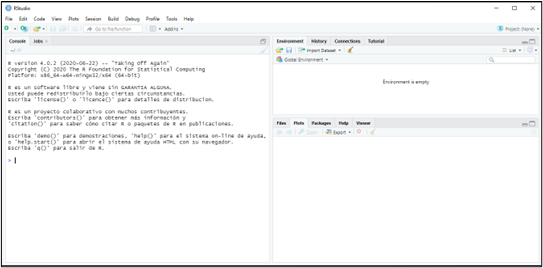
\includegraphics[width=5.20833in,height=\textheight]{figuras/Imagen1_01.png}
\caption{\textsc{IDE de RStudio.}}
\end{figure}

La parte izquierda de la ventana es la \textbf{consola}. La consola es la sección de RStudio donde podemos manejar R mediante la introducción de código. Por ejemplo, podemos escribir \texttt{2+2} después del cursor (signo ``\textgreater{}''), y pulsar Enter. La propia consola nos devolverá el valor 4:

\begin{Shaded}
\begin{Highlighting}[]
\DecValTok{2}\SpecialCharTok{+}\DecValTok{2}
\end{Highlighting}
\end{Shaded}

\begin{verbatim}
## [1] 4
\end{verbatim}

De todos modos, la forma más eficiente de trabajar es mediante ``proyectos'' y ``scripts''.

Un \textbf{proyecto} básicamente viene asociado a la carpeta donde R trabajará, buscando los datos que sean sus ``inputs'', y, en su caso, enviando sus resultados u ``outputs''. Dicho de otro modo, es una carpeta más de nuestro sistema de carpetas o directorios; pero a la que dotamos de una característica especial: ser un proyecto de R. Si abrimos desde RStudio el proyecto, estaremos diciendo a R que, por defecto, preferentemente busque todos los archivos e inputs (datos, etc.) que necesite en esa carpeta de proyecto; y que, en su caso, guarde en tal carpeta los outputs que genere.

Para crear un nuevo proyecto, seguiremos la instrucción \texttt{File\ →\ New\ Project}, luego se nos preguntará si se crea el proyecto en una nueva carpeta o en una ya existente. Vamos a crearlo, por ejemplo, en el disco extraíble D, carpeta R, subcarpeta ``explora'', que ya está creada. Nos saldrá una ventana para buscar la carpeta y, cuando la encontremos, pulsaremos \texttt{Open} y \texttt{Create\ Project}. Ya tendremos creado nuestro proyecto. Si nos vamos al explorador de Windows®, y buscamos la carpeta ``explora'', encontraremos que en tal carpeta aparece un archivo de nombre ``explora'', con un icono de un cubo con una ``R''. Ese archivo lo que está haciendo es actuar como un ``faro'' que le dice a R que, cuando trabajemos en el proyecto ``explora'', todos los archivos de datos necesarios estarán en esa carpeta (también llamada ``explora'', porque el proyecto adopta el nombre de la carpeta donde lo localizamos). Y que, si nuestro trabajo aporta algún fichero de ``output'', también se depositará en esa carpeta del proyecto.

En futuras sesiones, si queremos trabajar en el mismo proyecto, en lugar de seguir la ruta \texttt{File\ →\ New\ Project}, tendremos que hacer \texttt{File\ →\ Open\ Project}.

\section{Scripts.}\label{scripts.}

En cuanto a los \textbf{scripts}, son programas o rutinas donde varias instrucciones se ejecutan secuencialmente. Para crear un script, se seguirá la ruta Fi\texttt{le\ →\ New\ File\ →\ R\ Script}. Y si el script lo guardamos, ¿dónde lo hará? Pues en la carpeta ``explora'', que es la del proyecto en el que estamos trabajando.

Informáticamente, un script es simplemente un archivo de texto plano. Se puede modificar con cualquier editor de texto. Afortunadamente, para no estar entrando y saliendo de R-Studio, esta interfaz incorpora un \textbf{editor} de scripts, lo cual es muy cómodo.

Vemos cómo ahora, a la izquierda de RStudio, ha aparecido, en la parte superior, una nueva ventana, pasando la consola a ocupar la parte inferior. Es la ventana del ``editor'':

\begin{figure}
\centering
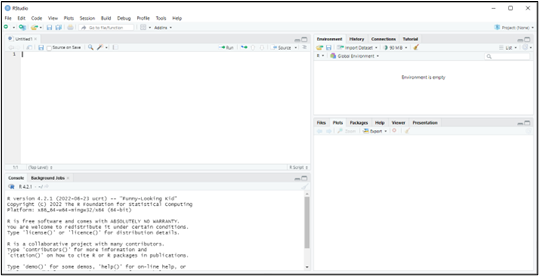
\includegraphics[width=5.20833in,height=\textheight]{figuras/Imagen1_02.png}
\caption{\textsc{El editor de Scripts de RStudio.}}
\end{figure}

Igual que con los proyectos, podemos crear desde RStudio un script nuevo, o abrir uno preexistente; y modificarlo, ejecutarlo, o volverlo a guardar.

Vamos a comenzar a escribir nuestro script. Si queremos hacer un comentario que no ejecute ninguna instrucción, éste irá precedido del símbolo almohadilla o \emph{hashtag} ``\#''. Luego, vamos a ordenar a R que haga la operación de suma: 2+2. Escribimos, por tanto, en el editor:

\begin{Shaded}
\begin{Highlighting}[]
\CommentTok{\#Ejemplo de Script}
\DecValTok{2}\SpecialCharTok{+}\DecValTok{2}  \CommentTok{\#este script hace una simple suma.}
\end{Highlighting}
\end{Shaded}

Si pulsamos \texttt{Control\ +\ Mayúsculas\ +\ ENTER} o al desplegable de \texttt{Source\ →\ Source\ with\ Echo}, se ejecutará el script (para ejecutar solo la línea donde está el cursor, pulsaremos \texttt{Control\ +\ ENTER} o el botón de \texttt{Run}; y para ejecutar varias líneas, hemos de sombrearlas y pulsar \texttt{Control\ +\ ENTER} o el botón de \texttt{Run}). En la consola aparecerá:

\begin{verbatim}
## [1] 4
\end{verbatim}

Podemos guardar el script con \texttt{File\ →\ Save\ As…} ¿Dónde se guardará por defecto? Pues en la carpeta ``explora'', que es la de nuestro proyecto. Una vez nuestro script ya tiene nombre, podemos ir guardándolo de vez en cuando pulsando simplemente en el botón del ``disquete'' del editor. Vamos a llamarlo, por ejemplo, ``explorando''. Si vamos, en el explorador de Windows®, a nuestra carpeta de proyecto, veremos que hay un archivo de texto llamado ``explorando'' con extensión ``.R'' (explorando.R). Este script lo podremos ejecutar cuantas veces queramos sin tener que escribir nada, o reescribirlo si vemos que no funciona o que necesitamos hacer modificaciones. Esa es la ventaja de trabajar con scripts.

Para recuperar un script en una nueva sesión de trabajo simplemente tenemos que seguir las instrucciones \texttt{File\ →\ Open\ File…} y seleccionarlo.

\section{Funciones.}\label{funciones.}

R trabaja con datos y funciones, principalmente. Pero, ¿qué es una \textbf{función}?

Una función es un conjunto o \textbf{sistema de instrucciones} que convierten unos datos de entrada o \textbf{inputs} en otros datos de salida, resultados, u \textbf{outputs}. Una función puede ser muy sencilla o ser verdaderamente compleja. Por otro lado, no todas las funciones están integradas en ``paquetes''; sino que el usuario puede crear sus propias funciones (por ejemplo, escribiéndolas en un script) y ejecutarlas.

Las partes básicas de una función son:

\begin{itemize}
\item
  \textbf{Entradas, inputs o argumentos:} son las diversas informaciones necesarias para realizar el procedimiento de la función. Los argumentos pueden ser introducidos por el usuario, o pueden venir dados por defecto, lo que quiere decir que, si el usuario no dota de valor a un argumento, este tomará automáticamente un valor prestablecido.
\item
  \textbf{Cuerpo:} está formado por un conjunto de instrucciones que transforman los \emph{inputs} o entradas en los \emph{outputs} o salidas. Si el cuerpo de la función está formado por varias instrucciones, éstas deben escribirse entre llaves \texttt{\{\ \}}.
\item
  \textbf{Salidas:} son los resultados u \emph{output} de la función. Si una función ofrece como salida varios tipos de \emph{objetos,} estos objetos suelen ser almacenados en una estructura de almacenaje de \emph{lista}.
\end{itemize}

Como ejemplo, vamos a integrar en nuestro script una función, llamada ``suma''. Esta función requerirá de dos entradas o argumentos (dos números cualesquiera), y ofrecerá, como resultado, salida u output; la suma de tales entradas. El código es:

\begin{Shaded}
\begin{Highlighting}[]
\NormalTok{suma }\OtherTok{\textless{}{-}} \ControlFlowTok{function}\NormalTok{(x, y) \{}
\NormalTok{  resultado }\OtherTok{\textless{}{-}}\NormalTok{ x }\SpecialCharTok{+}\NormalTok{ y}
  \FunctionTok{return}\NormalTok{(resultado)}
\NormalTok{\}}
\end{Highlighting}
\end{Shaded}

Ahora, una vez ejecutado el código anterior; si queremos sumar, por ejemplo, los números 12 y 16, solo tendremos que teclear en la consola, o escribir en el script y hacer run, a la línea:

\begin{Shaded}
\begin{Highlighting}[]
\FunctionTok{suma}\NormalTok{(}\AttributeTok{x=}\DecValTok{12}\NormalTok{, }\AttributeTok{y=}\DecValTok{16}\NormalTok{)}
\end{Highlighting}
\end{Shaded}

\begin{verbatim}
## [1] 28
\end{verbatim}

\section{Paquetes (packages).}\label{paquetes-packages.}

R es un lenguaje de programación en torno al cual se ha desarrollado una cantidad casi inimaginable de recursos: funciones, bases de datos, utilidades\ldots{} Tal es la cantidad de recursos, que no sería operativo abrir R (directamente, o a través de una IDE, como RStudio) y tener inmediatamente todos esos recursos activos y preparados para ser utilizados. Además, R debería ser actualizado de un modo casi constante.

Por todo ello, todos los recursos disponibles están organizados mediante ``paquetes'' (``packages'' en inglés). Un \textbf{paquete} es una colección de funciones y/o un conjunto de datos desarrollados por la comunidad de R. Estos incrementan el potencial de R ampliando sus capacidades básicas, o añadiendo otras nuevas.

De hecho, cuando abrimos R, algunos de estos paquetes, que se han instalado junto al propio lenguaje, se activan. Pero solo algunos. Un ejemplo es el paquete \texttt{\{base\}} o el paquete \texttt{\{stats\}} (\citeproc{ref-R-base}{R Core Team 2024}).

La mayor parte de los paquetes disponibles no forman parte, por ``defecto'', en la misma instalación de R. Se encuentran en diversos servidores llamados repositorios. El más importante, es \href{https://cran.r-project.org/}{CRAN}, que es el ``repositorio oficial'' y que alberga más de 10.000 paquetes. Pero existen otros repositorios, a destacar, por ejemplo, GitHub.

Para \textbf{instalar} un paquete en nuestra máquina que esté albergado en CRAN, un modo sencillo es, dentro de R-Studio, pulsar en la ventana inferior / izquierda sobre la pestaña ``Packages'', y sobre el botón ``Install''. Emergerá entonces una ventana donde hay un campo para escribir el nombre del paquete (al comenzar a escribirlo, el propio R-Studio te sugerirá los paquetes disponibles). Esto equivale a usar (bien directamente en la consola, o bien como línea de código insertada en un script) la instrucción \texttt{install.packages()}, con el nombre del paquete entre comillas (si son varios, pues irán separados por comas.

Una vez se tiene instalado el paquete, ya no habrá que volver a instalarlo para utilizarlo; sino \textbf{activarlo}. De hecho, todos los paquetes que no se encuentran por defecto en la propia instalación de R, deben ser activados para poder usar sus funcionalidades y/o datos. Para hacerlo, se debe utilizar la instrucción \texttt{library()}, y el nombre del paquete dentro del paréntesis.

Del nombre de esta instrucción surge la confusión común de tomar como sinónimos las palabras ``paquete'' y ``librería'' en el entorno de R. Si nos referimos a estas colecciones de funcionalidades y/o datos; lo correcto es ``paquete'', ya que ``librería'' tiene más que ver con la organización informática de un software.

\section{Help! (sistema de ayuda).}\label{help-sistema-de-ayuda.}

A veces podemos albergar dudas sobre la correcta utilización de las funcionalidades y herramientas que nos proporciona un paquete. Hay varias fuentes de ayuda para intentar encontrar respuesta a las cuestiones que se nos plantean.

Una opción, para obtener información general sobre un paquete, es utilizar la función \texttt{help()}, con el argumento ``package''. Por ejemplo:

\begin{Shaded}
\begin{Highlighting}[]
\FunctionTok{help}\NormalTok{(}\AttributeTok{package=}\StringTok{"base"}\NormalTok{)}
\end{Highlighting}
\end{Shaded}

Observaremos como en la ventana inferior / izquierda de R-Studio nos saldrá la información correspondiente. De hecho, en tal ventana existe una pestaña \textbf{``Help''} para obtener la ayuda sin teclear código.

Además, cada función puede ser consultada individualmente mediante \texttt{help("nombre\ de\ la\ función")} o \texttt{help(function,\ package\ =\ "package")} si el paquete no ha sido cargado. Estas instrucciones nos mostrarán la descripción de la función y sus argumentos acompañados de ejemplos de utilización. Por ejemplo:

\begin{Shaded}
\begin{Highlighting}[]
\FunctionTok{help}\NormalTok{(}\StringTok{"rm"}\NormalTok{, }\AttributeTok{package=}\StringTok{"base"}\NormalTok{)}
\end{Highlighting}
\end{Shaded}

La instrucción anterior nos aporta la documentación sobre la función \texttt{rm()} del paquete \texttt{\{base\}} de R (nota: este paquete se activa por defecto al abrir R o R-Studio; por lo que el segundo argumento, con el nombre del paquete que contiene la instrucción no es necesario).

Otra opción para mostrar información de ayuda es la exploración de las ``viñetas'' (vignettes). Las \textbf{viñetas} son documentos que muestran de un modo más detallado las funcionalidades de un paquete. La información de las viñetas de un paquete están disponibles en el archivo ``documentation''. Puede obtenerse una lista de las viñetas de nuestros paquetes instalados con la función \texttt{browseVignettes()}. Si solo queremos consultar las viñetas de un paquete concreto pasaremos como argumento a la función el nombre del mismo: \texttt{browseVignettes(package\ =\ "packagename")}. En ambos casos, una ventana del navegador se abrirá para que podamos fácilmente explorar el documento.

Si optamos por permanecer en la consola, la instrucción \texttt{vignette()} nos mostrará una lista de viñetas, \texttt{vignette(package\ =\ "packagename")} las viñetas incluidas en el paquete, y una vez identificada la viñeta de interés podremos consultarla mediante \texttt{vignette("vignettename")}.

\chapter{Almacenando y manipulando datos.}\label{almacenando-y-manipulando-datos.}

\section{Objetos. Datos.}\label{objetos.-datos.}

Como vimos en el capítulo 1, tras ejecutar un sencillo script (o al escribir instrucciones directamente desde la consola), R es interactivo: responde a las entradas que recibe. Las entradas o \textbf{expresiones} pueden ser, básicamente:

\begin{itemize}
\item
  Expresiones aritméticas.
\item
  Expresiones lógicas.
\item
  Llamadas a funciones.
\item
  Asignaciones.
\end{itemize}

Las expresiones realizan acciones sobre \textbf{objetos} de R. Los objetos en R son entes que tienen ciertas características, \emph{metadatos}, llamados atributos. No todos los objetos tienen los mismos atributos y, ni tan siquiera, todos los objetos tienen atributos que los caractericen.

Los objetos más importantes en R son ciertas estructuras o \emph{contenedores} diseñados para almacenar elementos:

\begin{itemize}
\item
  Vectores.
\item
  Matrices.
\item
  Listas.
\item
  Data frames.
\item
  Factores.
\end{itemize}

Los elementos almacenados en los objetos se dividen en \emph{clases}. Entre las diferentes clases, destacan las clases referidas a \textbf{datos}, que pueden ser de diferentes \emph{modos}: logical (verdadero/falso), numeric (números) o character (cadena de texto). El modo numeric puede ser, a la vez, de tipo integer (número entero) o double (número real). En el caso de logical y carácter, modo y tipo coinciden.

Vamos a profundizar un poco en algunas de estos contenedores de datos. Vamos a suponer que trabajamos en el proyecto que creamos en el capítulo anterior (proyecto ``explora''), y que vamos a editar el script que también creamos en tal capítulo (script ``explorando.R'', que se encontrará ubicado en la carpeta del proyecto ``explora'').

\subsection{Vectores.}\label{vectores.}

Los \textbf{vectores}, son conjuntos de elementos \textbf{de la misma clase}. Vamos a definir por ejemplo el vector x = (1,3,5,8). Para ello, vamos a escribir en nuestro script:

\begin{Shaded}
\begin{Highlighting}[]
\NormalTok{x }\OtherTok{\textless{}{-}} \FunctionTok{c}\NormalTok{(}\DecValTok{1}\NormalTok{,}\DecValTok{3}\NormalTok{,}\DecValTok{5}\NormalTok{,}\DecValTok{8}\NormalTok{)}
\end{Highlighting}
\end{Shaded}

Ejecutamos la línea (situando el cursor en algún lugar de ella, dentro del script; y pulsando a la vez las teclas \texttt{Control\ +\ Enter} o pinchando con el ratón en el botón \texttt{Run} del editor). Ya tenemos nuestro primer objeto de tipo \emph{vector} en memoria. Por cierto, lo que hemos hecho es una \textbf{asignación}, que se escribe con una flecha creada mediante los signos ``\textless{}'' y ``-''. Hemos asignado a un vector llamado ``x'' los elementos 1, 3, 5 y 8.

Para ver el vector simplemente escribimos en la consola (o en el script) el nombre del vector, ``x''. El resultado será:

\begin{verbatim}
## [1] 1 3 5 8
\end{verbatim}

Además, si miramos en la ventana superior-derecha de R-Studio, veremos que en el \textbf{\emph{Global Environment}} se muestra nuestro vector y que, además, se nos informa de que tiene \emph{modo} \emph{numérico}. El \emph{Global Environment} nos informa de los objetos que R tiene en memoria:

\begin{figure}
\centering
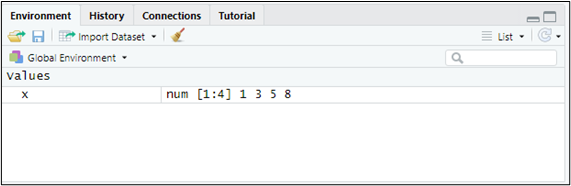
\includegraphics[width=5.20833in,height=\textheight]{figuras/Imagen2_01.png}
\caption{Nuestro vector en memoria.}
\end{figure}

Si queremos obtener un vector de números consecutivos del 2 al 6, basta con ejecutar en la ``consola'' (o escribir y ejecutar en el script):

\begin{Shaded}
\begin{Highlighting}[]
\NormalTok{y }\OtherTok{\textless{}{-}} \FunctionTok{c}\NormalTok{(}\DecValTok{2}\SpecialCharTok{:}\DecValTok{6}\NormalTok{)}
\end{Highlighting}
\end{Shaded}

Al escribir el nombre del vector ``y'' en la ``consola'' obtendremos:

\begin{Shaded}
\begin{Highlighting}[]
\NormalTok{y}
\end{Highlighting}
\end{Shaded}

\begin{verbatim}
## [1] 2 3 4 5 6
\end{verbatim}

Si queremos saber la longitud de un vector, usaremos la \emph{función} \texttt{length()}. Por ejemplo, \texttt{length(y)} nos devolverá el valor 5. Escribamos en el script y ejecutemos:

\begin{Shaded}
\begin{Highlighting}[]
\FunctionTok{length}\NormalTok{(y)}
\end{Highlighting}
\end{Shaded}

\begin{verbatim}
## [1] 5
\end{verbatim}

Un vector puede incluir, además de números, caracteres o grupos de caracteres alfanuméricos; siempre entrecomillados (lo fundamental es que sean elementos de la misma clase). Por ejemplo, el vector ``genero'' (¡no pongamos tildes o podemos tener problemas!). Así, si ejecutamos estas dos líneas de código:

\begin{Shaded}
\begin{Highlighting}[]
\NormalTok{genero}\OtherTok{\textless{}{-}}\FunctionTok{c}\NormalTok{(}\StringTok{"Mujer"}\NormalTok{,}\StringTok{"Hombre"}\NormalTok{)}
\NormalTok{genero}
\end{Highlighting}
\end{Shaded}

Se habrá creado el vector ``genero'':

\begin{verbatim}
## [1] "Mujer"  "Hombre"
\end{verbatim}

Podemos obtener la clase de los elementos almacenados en nuestro vector con la función \texttt{class()}:

\begin{Shaded}
\begin{Highlighting}[]
\FunctionTok{class}\NormalTok{(genero)}
\end{Highlighting}
\end{Shaded}

\begin{verbatim}
## [1] "character"
\end{verbatim}

Si falta un dato en un vector, habrá que escribir ``NA'' (not available). Por ejemplo, si falta el tercer dato de este vector ``z'', este vector se escribirá como:

\begin{Shaded}
\begin{Highlighting}[]
\NormalTok{Z }\OtherTok{\textless{}{-}} \FunctionTok{c}\NormalTok{(}\DecValTok{1}\NormalTok{,}\DecValTok{2}\NormalTok{,}\ConstantTok{NA}\NormalTok{,}\DecValTok{2}\NormalTok{,}\DecValTok{8}\NormalTok{)}
\end{Highlighting}
\end{Shaded}

Para \textbf{seleccionar un elemento} concreto de un vector, indicaremos entre corchetes la posición en la que se encuentra. Por ejemplo, refiriéndonos al vector ``x'', para obtener el valor de su tercer elemento, haremos:

\begin{Shaded}
\begin{Highlighting}[]
\NormalTok{x[}\DecValTok{3}\NormalTok{]}
\end{Highlighting}
\end{Shaded}

\begin{verbatim}
## [1] 5
\end{verbatim}

Si queremos que se nos muestre los elementos del vector x del 2º al 4º:

\begin{Shaded}
\begin{Highlighting}[]
\NormalTok{x[}\DecValTok{2}\SpecialCharTok{:}\DecValTok{4}\NormalTok{]}
\end{Highlighting}
\end{Shaded}

\begin{verbatim}
## [1] 3 5 8
\end{verbatim}

Por último, si queremos sacar en pantalla los elementos 1º y 4º, tendremos que incluir una ``c'' seguida de un paréntesis que recoja el orden de los elementos que queremos seleccionar:

\begin{Shaded}
\begin{Highlighting}[]
\NormalTok{x[}\FunctionTok{c}\NormalTok{(}\DecValTok{1}\NormalTok{,}\DecValTok{4}\NormalTok{)]}
\end{Highlighting}
\end{Shaded}

\begin{verbatim}
## [1] 1 8
\end{verbatim}

\subsection{Matrices.}\label{matrices.}

Las \textbf{matrices}, internamente en R, son vectores; pero con dos atributos adicionales: número de filas y número de columnas. Se definen mediante la función matrix(). Por ejemplo, para definir la matriz ``a'':

\[
\begin{pmatrix}
    1 & 4 & 7 \\
    2 & 5 & 8 \\
    3 & 6 & 9
\end{pmatrix}
\] Tendremos que escribir:

\begin{Shaded}
\begin{Highlighting}[]
\NormalTok{a }\OtherTok{\textless{}{-}} \FunctionTok{matrix}\NormalTok{(}\FunctionTok{c}\NormalTok{(}\DecValTok{1}\NormalTok{,}\DecValTok{2}\NormalTok{,}\DecValTok{3}\NormalTok{,}\DecValTok{4}\NormalTok{,}\DecValTok{5}\NormalTok{,}\DecValTok{6}\NormalTok{,}\DecValTok{7}\NormalTok{,}\DecValTok{8}\NormalTok{,}\DecValTok{9}\NormalTok{),}\AttributeTok{nrow=}\DecValTok{3}\NormalTok{)}
\NormalTok{a}
\end{Highlighting}
\end{Shaded}

\begin{verbatim}
##      [,1] [,2] [,3]
## [1,]    1    4    7
## [2,]    2    5    8
## [3,]    3    6    9
\end{verbatim}

El número de filas de la matriz (y por tanto, el número de columnas) se fija con el argumento \texttt{nrow\ =} . También podríamos fijar el número de columnas, con \texttt{ncol\ =} .

Como vemos, por defecto, R va ``cortando'' el vector por columnas (si lo preferimos, lo puede hacer también por filas, añadiendo a la función \texttt{matrix()} el argumento \texttt{by\ row\ =\ true}; pero, en nuestro ejemplo, obtendríamos la matriz traspuesta a la que queremos almacenar).

Las dimensiones (número de filas y de columnas) de la matriz pueden obtenerse mediante la función \texttt{dim()}:

\begin{Shaded}
\begin{Highlighting}[]
\FunctionTok{dim}\NormalTok{(a)}
\end{Highlighting}
\end{Shaded}

\begin{verbatim}
## [1] 3 3
\end{verbatim}

3 filas y 3 columnas.

Si queremos seleccionar elementos concretos de una matriz, lo haremos utilizando corchetes para indicar filas y columnas. Hemos de tener en cuenta que, trabajando con matrices, siempre tenemos \[rango de filas, rango de columnas\] Si se deja en blanco el espacio entre el corchete inicial y la coma, esto querrá decir que consideramos todas las filas. Y si no insertamos nada entre la coma y el corchete de cierre, esto significará que consideramos todas las columnas. A continuación tenemos varios ejemplos de código, con el resultado obtenido en la consola:

\begin{Shaded}
\begin{Highlighting}[]
\NormalTok{a[}\DecValTok{2}\NormalTok{,}\DecValTok{3}\NormalTok{]}
\end{Highlighting}
\end{Shaded}

\begin{verbatim}
## [1] 8
\end{verbatim}

\begin{Shaded}
\begin{Highlighting}[]
\NormalTok{a[}\DecValTok{1}\SpecialCharTok{:}\DecValTok{2}\NormalTok{,}\DecValTok{2}\SpecialCharTok{:}\DecValTok{3}\NormalTok{] }
\end{Highlighting}
\end{Shaded}

\begin{verbatim}
##      [,1] [,2]
## [1,]    4    7
## [2,]    5    8
\end{verbatim}

\begin{Shaded}
\begin{Highlighting}[]
\NormalTok{a[,}\FunctionTok{c}\NormalTok{(}\DecValTok{1}\NormalTok{,}\DecValTok{3}\NormalTok{)]}
\end{Highlighting}
\end{Shaded}

\begin{verbatim}
##      [,1] [,2]
## [1,]    1    7
## [2,]    2    8
## [3,]    3    9
\end{verbatim}

\begin{Shaded}
\begin{Highlighting}[]
\NormalTok{a[}\FunctionTok{c}\NormalTok{(}\DecValTok{1}\NormalTok{,}\DecValTok{3}\NormalTok{),]}
\end{Highlighting}
\end{Shaded}

\begin{verbatim}
##      [,1] [,2] [,3]
## [1,]    1    4    7
## [2,]    3    6    9
\end{verbatim}

Tanto para vectores como para matrices, funcionan las operaciones suma y diferencia sin más complicaciones. En el caso del producto, sin embargo, hay que tener en cuenta que, por ejemplo, a*a devuelve la multiplicación elemento a elemento, es decir:

\begin{Shaded}
\begin{Highlighting}[]
\NormalTok{a}\SpecialCharTok{*}\NormalTok{a}
\end{Highlighting}
\end{Shaded}

Devuelve la multiplicación elemento a elemento (en este caso, el cuadrado de cada número, al multiplicar la matriz a por sí misma):

\begin{verbatim}
##      [,1] [,2] [,3]
## [1,]    1   16   49
## [2,]    4   25   64
## [3,]    9   36   81
\end{verbatim}

Para hacer el verdadero producto matricial deberá introducirse:

\begin{Shaded}
\begin{Highlighting}[]
\NormalTok{a}\SpecialCharTok{\%*\%}\NormalTok{a}
\end{Highlighting}
\end{Shaded}

\begin{verbatim}
##      [,1] [,2] [,3]
## [1,]   30   66  102
## [2,]   36   81  126
## [3,]   42   96  150
\end{verbatim}

\subsection{Data frames.}\label{data-frames.}

Un \textbf{\emph{data frame}} es un objeto que almacena datos organizados mediante la clase \texttt{data.frame}. Esta organización consiste en que, por filas, se disponen los diferentes casos o sujetos; mientras que por columnas se posicionan las variables. Así:

\begin{itemize}
\item
  Es similar a una matriz en el sentido de que tiene dos dimensiones. Podemos acceder a sus elementos con corchetes, tenemos nombres de filas y columnas, y podemos operar con ellas.
\item
  Cada columna tiene un nombre, de manera que podemos acceder a una columna concreta con el símbolo \textbf{\texttt{\$}}. Todas las columnas (variables) son vectores con la misma longitud.
\item
  Cada columna puede ser un vector numérico, factor, de tipo carácter o lógico.
\end{itemize}

Por ejemplo, vamos a crear el \emph{data frame} \textbf{``datos''}, con tres variables: ``peso'', ``altura'', y ``color de ojos'', llamadas ``Peso'', ``Altura'' y ``Cl.ojos'', respectivamente; para 3 individuos o casos. Una opción es crear primero las tres variables como vectores, y luego crear el \emph{data frame} mediante la función \texttt{dataframe()}:

\begin{Shaded}
\begin{Highlighting}[]
\NormalTok{Peso}\OtherTok{\textless{}{-}}\FunctionTok{c}\NormalTok{(}\DecValTok{68}\NormalTok{,}\DecValTok{75}\NormalTok{,}\DecValTok{88}\NormalTok{)}
\NormalTok{Altura}\OtherTok{\textless{}{-}}\FunctionTok{c}\NormalTok{(}\FloatTok{1.6}\NormalTok{,}\FloatTok{1.8}\NormalTok{,}\FloatTok{1.9}\NormalTok{)}
\NormalTok{Cl.ojos}\OtherTok{\textless{}{-}}\FunctionTok{c}\NormalTok{(}\StringTok{"azules"}\NormalTok{,}\StringTok{"marrones"}\NormalTok{,}\StringTok{"marrones"}\NormalTok{)}
\NormalTok{datos}\OtherTok{\textless{}{-}}\FunctionTok{data.frame}\NormalTok{(Peso,Altura,Cl.ojos)}
\end{Highlighting}
\end{Shaded}

Si ahora ejecutamos una línea con el nombre de nuestro \emph{data frame}, lo obtendremos como resultado en la consola:

\begin{Shaded}
\begin{Highlighting}[]
\NormalTok{datos}
\end{Highlighting}
\end{Shaded}

\begin{verbatim}
##   Peso Altura  Cl.ojos
## 1   68    1.6   azules
## 2   75    1.8 marrones
## 3   88    1.9 marrones
\end{verbatim}

Para obtener los nombres de las variables (es decir, el nombre de cada columna) teclearemos la función:

\begin{Shaded}
\begin{Highlighting}[]
\FunctionTok{names}\NormalTok{(datos)}
\end{Highlighting}
\end{Shaded}

Obteniéndose:

\begin{verbatim}
## [1] "Peso"    "Altura"  "Cl.ojos"
\end{verbatim}

Para obtener solo los datos de la columna (variable) color de ojos teclearemos datos\$Cl.ojos:

\begin{Shaded}
\begin{Highlighting}[]
\NormalTok{datos}\SpecialCharTok{$}\NormalTok{Cl.ojos}
\end{Highlighting}
\end{Shaded}

\begin{verbatim}
## [1] "azules"   "marrones" "marrones"
\end{verbatim}

Y para obtener los datos de peso: datos\$Peso:

\begin{Shaded}
\begin{Highlighting}[]
\NormalTok{datos}\SpecialCharTok{$}\NormalTok{Peso}
\end{Highlighting}
\end{Shaded}

\begin{verbatim}
## [1] 68 75 88
\end{verbatim}

Para saber el número de filas y de columnas de una hoja de datos utilizaremos las funciones \texttt{nrow()} y \texttt{ncol()}:

\begin{Shaded}
\begin{Highlighting}[]
\FunctionTok{nrow}\NormalTok{(datos)}
\end{Highlighting}
\end{Shaded}

\begin{verbatim}
## [1] 3
\end{verbatim}

\begin{Shaded}
\begin{Highlighting}[]
\FunctionTok{ncol}\NormalTok{(datos)}
\end{Highlighting}
\end{Shaded}

\begin{verbatim}
## [1] 3
\end{verbatim}

Para seleccionar elementos de un data frame, se pueden seguir las mismas reglas que para la selección de elementos de una matriz (con el número de cada fila, que es cada individuo; y el número de cada columna, que es cada variable. Para elegir una variable, no obstante, ya hemos visto que es posible usar su nombre; aunque precedido del nombre del data frame y el signo \texttt{\$}. Por ejemplo, si ejecutamos:

\begin{Shaded}
\begin{Highlighting}[]
\NormalTok{datos[,}\DecValTok{2}\NormalTok{]}
\end{Highlighting}
\end{Shaded}

\begin{verbatim}
## [1] 1.6 1.8 1.9
\end{verbatim}

\begin{Shaded}
\begin{Highlighting}[]
\NormalTok{datos}\SpecialCharTok{$}\NormalTok{Altura}
\end{Highlighting}
\end{Shaded}

\begin{verbatim}
## [1] 1.6 1.8 1.9
\end{verbatim}

Obtenemos el mismo resultado.

\section{Importando datos.}\label{importando-datos.}

Lo más frecuente es que no tecleemos los datos, como hemos hecho hasta ahora; sino que los importemos a R desde algún contenedor externo (archivo de texto, hoja de cálculo, base de datos\ldots). Nosotros vamos a importar nuestros datos desde Microsoft® Excel®. Vamos a cerrar el script que hemos estado construyendo en los apartados anteriores (para conservarlo hay que guardarlo antes), aunque vamos a seguir trabajando en el mismo proyecto (que habíamos llamado ``explora''). Iremos a la carpeta del proyecto y guardaremos en ella los dos archivos de esta práctica (obtén el enlace a los archivos en la sección final del capítulo):

\begin{itemize}
\item
  Un archivo de Microsoft® Excel® llamado ``eolica\_20.xlsx''
\item
  Un script con las instrucciones que vamos a mostrar a continuación, y que se llama ``explora\_eolica.R''
\end{itemize}

Si abrimos el archivo de Microsoft® Excel® comprobaremos que se compone de tres hojas. La primera muestra el criterio de búsqueda de casos en la un aviso sobre el uso exclusivo que se debe dar a los datos incorporados; la segunda recoge la descripción de las variables consideradas; y la tercera (hoja ``Top 20'') guarda los datos que debemos \textbf{importar} desde R-Studio. Estos datos se corresponden con diferentes variables económico-financieras de 20 empresas productoras de electricidad mediante generación eólica. Luego vamos a cerrar el archivo de Microsoft® Excel® y volveremos a R-Studio. Vamos a abrir nuestro script ``explora\_eolica.R'' con \texttt{File\ →\ Open\ File…} Este script contiene el programa que vamos a ir ejecutando en la práctica. La primera línea / instrucción en los scripts suele ser:

\begin{Shaded}
\begin{Highlighting}[]
\FunctionTok{rm}\NormalTok{(}\AttributeTok{list =} \FunctionTok{ls}\NormalTok{())}
\end{Highlighting}
\end{Shaded}

La instrucción tiene como objeto limpiar el \emph{Environment} (memoria) de objetos de anteriores sesiones de trabajo. Para importar los datos localizados en el archivo de Excel ``eolica\_20.xlsx'' el código es:

\begin{Shaded}
\begin{Highlighting}[]
\CommentTok{\# DATOS}
\FunctionTok{library}\NormalTok{(readxl)}
\NormalTok{eolica\_20 }\OtherTok{\textless{}{-}} \FunctionTok{read\_excel}\NormalTok{(}\StringTok{"eolica\_20.xlsx"}\NormalTok{, }\AttributeTok{sheet =} \StringTok{"Top 20"}\NormalTok{)}
\end{Highlighting}
\end{Shaded}

¡Atención! Si nunca se ha utilizado el paquete \texttt{\{readxl\}} (que contiene el código necesario para importar datos de un archivo de Microsoft® Excel®), cuando la intentemos activar con la función \texttt{library()} nos dará un error o nos dirá que previamente hay que importarla. En ese caso, iremos a la ventana inferior-derecha y pulsaremos la pestaña \texttt{Packages}, pulsaremos en \texttt{Install}, y emergerá una ventana donde dejaremos el ``repositorio'' que viene por defecto y, en el campo ``Packages'', escribiremos el nombre del ``paquete'' que contiene la librería que nos hace falta (normalmente coincide con el nombre de la propia librería, en nuestro caso \texttt{\{readxl\}}. Una vez descargado el ``paquete'', podremos ejecutar el código anterior sin problemas.

Otra cuestión importante a tener en cuenta es que, en la hoja de cálculo del ejemplo, los ``valores perdidos'' o \emph{missing values} (celdas en las que no hay datos), venían en blanco. Pero, en ocasiones, pueden contener algún tipo de anotación, como por ejemplo, ``n.d.'' (no disponible). En tal caso, deberá incluirse un argumento más que informe de estas celdas que, sin estar en blanco, no tienen dato:

\begin{Shaded}
\begin{Highlighting}[]
\NormalTok{eolica\_20 }\OtherTok{\textless{}{-}} \FunctionTok{read\_excel}\NormalTok{(}\StringTok{"eolica\_20.xlsx"}\NormalTok{, }\AttributeTok{sheet =} \StringTok{"Top 20"}\NormalTok{, }\AttributeTok{na =} \FunctionTok{c}\NormalTok{(}\StringTok{"n.d."}\NormalTok{))}
\end{Highlighting}
\end{Shaded}

Volviendo a nuestro ejemplo, podemos observar cómo en el \emph{Environment} ya aparece un objeto. Este objeto es una estructura de datos tipo \emph{data frame}, se llama ``eolica\_20'' y contiene 11 columnas, una por cada una de las variables almacenadas en el archivo de Microsoft® Excel®. De estas variables, tres son de tipo cualitativo, formadas por cadenas de caracteres: el nombre de la empresa, ``NOMBRE''; y el nombre del grupo empresarial matriz al que pertenece, ``MATRIZ''. Puede explorarse el contenido del \emph{data frame} y los principales estadísticos con la función \texttt{summary()}:

\begin{Shaded}
\begin{Highlighting}[]
\FunctionTok{summary}\NormalTok{ (eolica\_20)}
\end{Highlighting}
\end{Shaded}

\begin{verbatim}
##     NOMBRE               RES             ACTIVO             FPIOS        
##  Length:20          Min.   : -5662   Min.   :  109024   Min.   : -77533  
##  Class :character   1st Qu.:  2865   1st Qu.:  187240   1st Qu.:  27615  
##  Mode  :character   Median :  7388   Median :  271636   Median :  77740  
##                     Mean   : 50754   Mean   : 1183599   Mean   : 563678  
##                     3rd Qu.: 21206   3rd Qu.:  813816   3rd Qu.: 219345  
##                     Max.   :727548   Max.   :13492812   Max.   :6904824  
##                     NA's   :1                                            
## 
##      RENECO            RENFIN            LIQUIDEZ          MARGEN       
##  Min.   :-2.8130   Min.   :-359.773   Min.   :0.0780   Min.   :-302.03  
##  1st Qu.: 0.8765   1st Qu.:   1.664   1st Qu.:0.7342   1st Qu.:  12.39  
##  Median : 3.6150   Median :  10.812   Median :1.2345   Median :  21.42  
##  Mean   : 2.9399   Mean   :  -3.450   Mean   :1.4200   Mean   :  16.40  
##  3rd Qu.: 4.7735   3rd Qu.:  25.312   3rd Qu.:1.5615   3rd Qu.:  38.56  
##  Max.   : 8.5860   Max.   :  52.261   Max.   :5.3300   Max.   : 208.36  
##  NA's   :1                                                              
## 
##    SOLVENCIA         APALANCA           MATRIZ         
##  Min.   :-40.74   Min.   :-6265.50   Length:20         
##  1st Qu.: 11.26   1st Qu.:   16.13   Class :character  
##  Median : 23.68   Median :  145.93   Mode  :character  
##  Mean   : 32.68   Mean   :  -17.17                     
##  3rd Qu.: 52.62   3rd Qu.:  504.74                     
##  Max.   : 99.08   Max.   : 1019.62
\end{verbatim}

Veremos cómo aparecen 11 variables con algunos estadísticos básicos.

R ha considerado la primera columna como una variable de tipo cualitativo (atributo). En realidad no es una variable, sino el nombre de los individuos o casos. Para evitar que R tome los nombres de los casos como una variable, podemos redefinir nuestro \emph{data frame} diciéndole que considere esa primera columna como los \emph{nombres de los individuos o filas}:

\begin{Shaded}
\begin{Highlighting}[]
\NormalTok{eolica\_20 }\OtherTok{\textless{}{-}} \FunctionTok{data.frame}\NormalTok{(eolica\_20, }\AttributeTok{row.names =} \DecValTok{1}\NormalTok{)}
\end{Highlighting}
\end{Shaded}

En la línea anterior hemos asignado al data frame ``eolica\_20'' los propios datos de ``eolica\_20''; pero indicando que la primera columna de datos no es una variable; sino el nombre de los casos. Si hacemos ahora el \texttt{summary()}:

\begin{verbatim}
##       RES             ACTIVO             FPIOS             RENECO       
##  Min.   : -5662   Min.   :  109024   Min.   : -77533   Min.   :-2.8130  
##  1st Qu.:  2865   1st Qu.:  187240   1st Qu.:  27615   1st Qu.: 0.8765  
##  Median :  7388   Median :  271636   Median :  77740   Median : 3.6150  
##  Mean   : 50754   Mean   : 1183599   Mean   : 563678   Mean   : 2.9399  
##  3rd Qu.: 21206   3rd Qu.:  813816   3rd Qu.: 219345   3rd Qu.: 4.7735  
##  Max.   :727548   Max.   :13492812   Max.   :6904824   Max.   : 8.5860  
##  NA's   :1                                             NA's   :1        
## 
##      RENFIN            LIQUIDEZ          MARGEN          SOLVENCIA     
##  Min.   :-359.773   Min.   :0.0780   Min.   :-302.03   Min.   :-40.74  
##  1st Qu.:   1.664   1st Qu.:0.7342   1st Qu.:  12.39   1st Qu.: 11.26  
##  Median :  10.812   Median :1.2345   Median :  21.42   Median : 23.68  
##  Mean   :  -3.450   Mean   :1.4200   Mean   :  16.40   Mean   : 32.68  
##  3rd Qu.:  25.312   3rd Qu.:1.5615   3rd Qu.:  38.56   3rd Qu.: 52.62  
##  Max.   :  52.261   Max.   :5.3300   Max.   : 208.36   Max.   : 99.08  
## 
##     APALANCA           MATRIZ         
##  Min.   :-6265.50   Length:20         
##  1st Qu.:   16.13   Class :character  
##  Median :  145.93   Mode  :character  
##  Mean   :  -17.17                     
##  3rd Qu.:  504.74                     
##  Max.   : 1019.62
\end{verbatim}

Vemos que ya no aparece ``NOMBRE'' como variable, y en el \emph{Environment} ya aparece el data frame ``eolica\_20'' con 20 observaciones (casos), pero con 10 variables (una menos).

Antes de seguir con la manipulación de nuestros datos, es preciso decir que existen otros muchos formatos de datos que pueden ser importados. Por ejemplo, con el paquete \texttt{\{readr\}} se pueden importar datos de archivos de texto de tipo tabular (por ejemplo, archivos *.csv). Con el paquete \texttt{\{haven\}} se pueden capturar los datos almacenados en archivos de SPSS® (.sav), Stata® (.dta), SAS® (.sas7bdat), etc. Finamente, se pueden capturar datos almacenados en páginas web (archivos en formato JSON o XML, o en tablas HTML)) o en bases de datos gestionadas mediante diversos sistemas (SQLite, MySQL, MariaDB, PostgreSQL, Oracle®).

\section{\{dplyr\}.}\label{dplyr.}

\subsection{El Tidyverse. Cargando \{dplyr\}.}\label{el-tidyverse.-cargando-dplyr.}

El \textbf{\emph{Tidyverse}} es un conjunto de paquetes / librerías con una filosofía común, como es el uso de ciertas estructuras gramaticales, que facilitan muchas de las tareas y análisis que podrían hacerse con el lenguaje R estándar. Una buena obra para profundizar en el Tidyverse es Wickham and Grolemund (\citeproc{ref-Wickham2017R}{2017}).

Uno de esos paquetes es \texttt{\{dplyr\}}, que proporciona una gramática más sencilla que la del lenguaje R convencional para \textbf{manipular} los objetos de estructuras de datos conocidos como \textbf{\emph{data frames}}.

Los data frames, como ya sabemos, son estructuras en las que se almacenan datos de modo que, por columnas, se disponen las variables del análisis; y por filas los casos que conforman la muestra / población.

Vamos a suponer que trabajamos dentro del proyecto que hemos creado previamente, de nombre ``explora'' (ver capítulo 1). Dentro de la carpeta del proyecto guardaremos el script llamado ``explora\_dplyr.R'' y el archivo de Microsoft® Excel® llamado ``eolica\_20.xlsx''. Si abrimos este último archivo, comprobaremos que se compone de tres hojas. La hoja ``Top 20'' contiene los datos a importar desde R-Studio. Estos datos se corresponden con diferentes variables económico-financieras de 20 empresas productoras de electricidad mediante generación eólica.

Luego cerraremos el archivo de Microsoft® Excel®, ``eolica\_20.xlsx'', y volveremos a R-Studio. Después, abriremos nuestro script ``explora\_dplyr.R'' con \texttt{File\ →\ Open\ File…} Este script contiene el programa que vamos a ir ejecutando en la práctica.

La primera línea / instrucción en los scripts suele ser:

\begin{Shaded}
\begin{Highlighting}[]
\FunctionTok{rm}\NormalTok{(}\AttributeTok{list =} \FunctionTok{ls}\NormalTok{())}
\end{Highlighting}
\end{Shaded}

La instrucción tiene como objeto limpiar el \emph{Environment} (memoria) de objetos de anteriores sesiones de trabajo.

Para importar los datos que hay en la hoja ``Top 20'' del archivo de Microsoft® Excel® llamado ``eolica\_20.xlsx'', ejecutaremos el código:

\begin{Shaded}
\begin{Highlighting}[]
\CommentTok{\# DATOS}

\FunctionTok{library}\NormalTok{(readxl)}
\NormalTok{eolica\_20 }\OtherTok{\textless{}{-}} \FunctionTok{read\_excel}\NormalTok{(}\StringTok{"eolica\_20.xlsx"}\NormalTok{, }\AttributeTok{sheet =} \StringTok{"Top 20"}\NormalTok{)}
\end{Highlighting}
\end{Shaded}

Podemos observar como en el \emph{Environment} ya aparece un objeto. Este objeto es una estructura de datos tipo \emph{data frame}, se llama ``eolica\_20'' y contiene 11 columnas. R ha considerado la primera columna como una variable de tipo cualitativo. En realidad, la primera columna no es una variable, sino que está formada por el nombre (identificador) de los diferentes casos u observaciones. Para evitar que R tome los nombres de los casos como una variable más, podemos redefinir nuestro \emph{data frame} diciéndole que tome esa primera columna como los \emph{nombres de los individuos}:

\begin{Shaded}
\begin{Highlighting}[]
\NormalTok{eolica\_20 }\OtherTok{\textless{}{-}} \FunctionTok{data.frame}\NormalTok{(eolica\_20, }\AttributeTok{row.names =} \DecValTok{1}\NormalTok{)}
\end{Highlighting}
\end{Shaded}

En la línea anterior hemos asignado al \emph{data frame} ``eolica\_20'' los propios datos de ``eolica\_20''; pero indicando que la primera columna de datos no es una variable; sino el nombre de los casos.

A continuación, cargaremos el paquete \texttt{\{dplyr\}}. Si nunca antes se ha utilizado este paquete, cuando lo intentemos activar con la función \texttt{library()} nos dará un error o nos dirá que previamente hay que importarlo. En ese caso, iremos a la ventana inferior-derecha y pulsaremos la pestaña ``Packages'', pulsaremos en \texttt{Install}, y emergerá una ventana donde dejaremos el ``repositorio'' que viene por defecto y, en el campo \texttt{Packages}, escribiremos el nombre del ``paquete'' (en nuestro caso \texttt{\{dplyr\}}). Una vez descargado el ``paquete'', podremos ejecutar el código sin problemas:

\begin{Shaded}
\begin{Highlighting}[]
\CommentTok{\#Cargando dplyr}

\FunctionTok{library}\NormalTok{ (dplyr)}
\end{Highlighting}
\end{Shaded}

Para entender mejor la \textbf{sintaxis} que siguen las funciones o instrucciones a las que da acceso \texttt{\{dplyr\}}, hay que tener en cuenta lo siguiente:

\begin{itemize}
\item
  El primer argumento que tiene una función de \texttt{\{dplyr\}} es el \emph{data frame} con el que se va a trabajar.
\item
  Los otros argumentos describen qué hay que hacer con el \emph{data frame} especificado en el primer argumento. Es posible referirse a las columnas (variables) del \emph{data frame} con su nombre, \textbf{sin utilizar el operador \$}.
\item
  El valor de retorno es un \textbf{nuevo} \emph{data frame}.
\end{itemize}

En los siguientes subapartados practicaremos con algunas de las principales funciones que aporta \texttt{\{dplyr\}}.

\subsection{Seleccionando columnas de un data frame.}\label{seleccionando-columnas-de-un-data-frame.}

La función clave de \texttt{\{dplyr\}} para seleccionar una o varias columnas (variables) de un \emph{data frame} es la función \texttt{select()}.

Así, vamos a imaginar por ejemplo que queremos eliminar de nuestro \emph{data frame} la variable (de tipo ``carácter'') MATRIZ. Podremos ejecutar la asignación:

\begin{Shaded}
\begin{Highlighting}[]
\CommentTok{\#Seleccionando variables}

\NormalTok{eolica\_20 }\OtherTok{\textless{}{-}}\FunctionTok{select}\NormalTok{(eolica\_20, }\SpecialCharTok{{-}}\NormalTok{MATRIZ)}
\FunctionTok{summary}\NormalTok{ (eolica\_20)}
\end{Highlighting}
\end{Shaded}

\begin{verbatim}
##       RES             ACTIVO             FPIOS        
##  Min.   : -5662   Min.   :  109024   Min.   : -77533  
##  1st Qu.:  2865   1st Qu.:  187240   1st Qu.:  27615  
##  Median :  7388   Median :  271636   Median :  77740  
##  Mean   : 50754   Mean   : 1183599   Mean   : 563678  
##  3rd Qu.: 21206   3rd Qu.:  813816   3rd Qu.: 219345  
##  Max.   :727548   Max.   :13492812   Max.   :6904824  
##  NA's   :1                                            
## 
##      RENECO            RENFIN            LIQUIDEZ     
##  Min.   :-2.8130   Min.   :-359.773   Min.   :0.0780  
##  1st Qu.: 0.8765   1st Qu.:   1.664   1st Qu.:0.7342  
##  Median : 3.6150   Median :  10.812   Median :1.2345  
##  Mean   : 2.9399   Mean   :  -3.450   Mean   :1.4200  
##  3rd Qu.: 4.7735   3rd Qu.:  25.312   3rd Qu.:1.5615  
##  Max.   : 8.5860   Max.   :  52.261   Max.   :5.3300  
##  NA's   :1                                            
## 
##      MARGEN          SOLVENCIA         APALANCA       
##  Min.   :-302.03   Min.   :-40.74   Min.   :-6265.50  
##  1st Qu.:  12.39   1st Qu.: 11.26   1st Qu.:   16.13  
##  Median :  21.42   Median : 23.68   Median :  145.93  
##  Mean   :  16.40   Mean   : 32.68   Mean   :  -17.17  
##  3rd Qu.:  38.56   3rd Qu.: 52.62   3rd Qu.:  504.74  
##  Max.   : 208.36   Max.   : 99.08   Max.   : 1019.62
\end{verbatim}

Podemos verificar que, en el \emph{Environment,} el \emph{data frame} ha pasado a tener una variable menos (9), ya que hemos eliminado la variable MATRIZ. Es decir, con el guión ``-'' se pueden eliminar directamente variables de un \emph{data frame}.

Ahora, suponemos que queremos visualizar las variables del \emph{data frame} ``eolica\_20'': ACTIVO, FPIOS, LIQUIDEZ, MARGEN, SOLVENCIA y APALANCA (es decir, todas las variables menos RES, RENECO, RENFIN). Para ello, ejecutaremos el código:

\begin{Shaded}
\begin{Highlighting}[]
\FunctionTok{select}\NormalTok{(eolica\_20, ACTIVO, FPIOS, LIQUIDEZ, MARGEN, SOLVENCIA, APALANCA)}
\end{Highlighting}
\end{Shaded}

\begin{verbatim}
##                                     ACTIVO       FPIOS LIQUIDEZ   MARGEN
## Holding De Negocios De GAS SL.  13492812.0 6904824.000    1.020   91.152
## Global Power Generation SA.      2002458.0 1740487.000    2.006   22.403
## Naturgy Renovables SLU           1956869.0  318475.000    1.263   20.442
## EDP Renovables España SLU        1275939.0  726783.000    1.596   47.193
## Corporacion Acciona Eolica SL     864606.0  136064.000    0.788   20.091
## Saeta Yield SA.                   796886.4  665319.556    2.687   16.258
## Elawan Energy SL.                 443467.0  186302.006    0.595  208.357
## Olivento SL                       381207.0   58340.998    0.771   16.629
## Parque Eolico La Boga SL.         303904.4   29316.797    1.407    1.001
## Naturgy Wind, S.L.                273542.0   28418.000    1.364   39.575
## Viesgo Renovables SL.             269730.0  177707.000    0.272   11.818
## Al-Andalus Wind Power SL          249853.8   21466.121    1.550   12.582
## Innogy Spain SA.                  230338.5   85447.212    1.416  -18.025
## Guzman Energia SL                 190287.0  -77532.698    0.078  -19.193
## Acciona Eolica Del Levante SL     188354.0   21769.000    2.855   27.520
## Biovent Energia SA                183899.0   70033.000    1.206   22.792
## Esquilvent SL                     157630.6   48769.130    5.330   39.476
## Eolica La Janda SL                153429.4   25206.748    1.184   38.256
## Parque Eolico Santa Catalina SL   147742.5   -1664.755    0.388   31.780
## WPD Wind Investment SL.           109023.8  108023.826    0.624 -302.027
## 
##                                 SOLVENCIA  APALANCA
## Holding De Negocios De GAS SL.     51.174    91.964
## Global Power Generation SA.        86.917     1.044
## Naturgy Renovables SLU             16.274   494.729
## EDP Renovables España SLU          56.960    67.028
## Corporacion Acciona Eolica SL      15.737   422.263
## Saeta Yield SA.                    83.489    17.067
## Elawan Energy SL.                  42.010   123.771
## Olivento SL                        15.304   534.761
## Parque Eolico La Boga SL.           9.646   921.591
## Naturgy Wind, S.L.                 10.388   824.537
## Viesgo Renovables SL.              65.883    13.330
## Al-Andalus Wind Power SL            8.591  1019.616
## Innogy Spain SA.                   37.096   150.688
## Guzman Energia SL                 -40.745  -343.542
## Acciona Eolica Del Levante SL      11.557   743.754
## Biovent Energia SA                 38.082   141.163
## Esquilvent SL                      30.938   218.275
## Eolica La Janda SL                 16.428   480.122
## Parque Eolico Santa Catalina SL    -1.126 -6265.496
## WPD Wind Investment SL.            99.082     0.000
\end{verbatim}

Como no hemos asignado el resultado de la función a ningún ``nombre'', R simplemente saca el resultado en pantalla; pero no guarda ningún objeto en el \emph{Environment}. Si asignamos un \texttt{select()} a un ``nombre'', se creará un \emph{data frame} con ese nombre, y las variables seleccionadas:

\begin{Shaded}
\begin{Highlighting}[]
\NormalTok{eolica\_20A }\OtherTok{\textless{}{-}}\FunctionTok{select}\NormalTok{(eolica\_20, ACTIVO, FPIOS, LIQUIDEZ, MARGEN, SOLVENCIA, APALANCA)}
\FunctionTok{summary}\NormalTok{ (eolica\_20A)}
\end{Highlighting}
\end{Shaded}

\begin{verbatim}
##       RES             ACTIVO             FPIOS        
##  Min.   : -5662   Min.   :  109024   Min.   : -77533  
##  1st Qu.:  2865   1st Qu.:  187240   1st Qu.:  27615  
##  Median :  7388   Median :  271636   Median :  77740  
##  Mean   : 50754   Mean   : 1183599   Mean   : 563678  
##  3rd Qu.: 21206   3rd Qu.:  813816   3rd Qu.: 219345  
##  Max.   :727548   Max.   :13492812   Max.   :6904824  
##  NA's   :1                                            
## 
##      RENECO            RENFIN            LIQUIDEZ     
##  Min.   :-2.8130   Min.   :-359.773   Min.   :0.0780  
##  1st Qu.: 0.8765   1st Qu.:   1.664   1st Qu.:0.7342  
##  Median : 3.6150   Median :  10.812   Median :1.2345  
##  Mean   : 2.9399   Mean   :  -3.450   Mean   :1.4200  
##  3rd Qu.: 4.7735   3rd Qu.:  25.312   3rd Qu.:1.5615  
##  Max.   : 8.5860   Max.   :  52.261   Max.   :5.3300  
##  NA's   :1                                            
## 
##      MARGEN          SOLVENCIA         APALANCA       
##  Min.   :-302.03   Min.   :-40.74   Min.   :-6265.50  
##  1st Qu.:  12.39   1st Qu.: 11.26   1st Qu.:   16.13  
##  Median :  21.42   Median : 23.68   Median :  145.93  
##  Mean   :  16.40   Mean   : 32.68   Mean   :  -17.17  
##  3rd Qu.:  38.56   3rd Qu.: 52.62   3rd Qu.:  504.74  
##  Max.   : 208.36   Max.   : 99.08   Max.   : 1019.62
\end{verbatim}

Podemos comprobar en el \emph{Environment} cómo hay otro objeto \emph{data frame} llamado ``eolica\_20A'', con 6 variables (y los mismos 20 casos). Este \emph{data frame} lo podríamos haber creado, también, eliminando del \emph{data frame} original (``eolica\_20''), las variables que nos sobran:

\begin{Shaded}
\begin{Highlighting}[]
\NormalTok{eolica\_20A }\OtherTok{\textless{}{-}}\FunctionTok{select}\NormalTok{(eolica\_20, }\SpecialCharTok{{-}}\NormalTok{RES, }\SpecialCharTok{{-}}\NormalTok{RENECO, }\SpecialCharTok{{-}}\NormalTok{RENFIN)}
\end{Highlighting}
\end{Shaded}

Más aún, si nos fijamos bien, los nombres de todas las variables que hemos excluido empiezan por ``RE'', a diferencia de las incluidas. Podríamos haber hecho también:

\begin{Shaded}
\begin{Highlighting}[]
\NormalTok{eolica\_20A }\OtherTok{\textless{}{-}}\FunctionTok{select}\NormalTok{(eolica\_20, }\SpecialCharTok{{-}}\NormalTok{(}\FunctionTok{starts\_with}\NormalTok{(}\StringTok{"RE"}\NormalTok{)))}
\end{Highlighting}
\end{Shaded}

Y de nuevo obtendríamos el mismo resultado. El argumento \texttt{starts\_with()} permite seleccionar variables cuyos nombres comienzan por cierta cadena de caracteres. También se puede hacer mismo con los caracteres finales (\texttt{ends\_with()}) o contenidos en alguna posición del nombre (\texttt{contains()}).

Otra posibilidad que tenemos es hacer una copia de un \emph{data frame} rápidamente con el argumento \texttt{everything()}. Por ejemplo:

\begin{Shaded}
\begin{Highlighting}[]
\NormalTok{eolica\_20\_replica }\OtherTok{\textless{}{-}}\FunctionTok{select}\NormalTok{(eolica\_20, }\FunctionTok{everything}\NormalTok{())}
\end{Highlighting}
\end{Shaded}

Se ha creado el \emph{date frame} ``eolica\_20\_replica'' que es una copia exacta de ``eolica\_20''.

\subsection{\texorpdfstring{Seleccionando casos de un \emph{data frame}.}{Seleccionando casos de un data frame.}}\label{seleccionando-casos-de-un-data-frame.}

Además de seleccionar variables, con \texttt{\{dplyr\}} también se pueden seleccionar casos que cumplan ciertas condiciones. La función para realizar este cometido es \texttt{filter()}. Por ejemplo, si queremos seleccionar las empresas eólicas con un resultado (variable RES) mayor o igual a 50.000 y presentarlas en pantalla, la instrucción será:

\begin{Shaded}
\begin{Highlighting}[]
\FunctionTok{filter}\NormalTok{(eolica\_20, RES }\SpecialCharTok{\textgreater{}=} \DecValTok{50000}\NormalTok{)}
\end{Highlighting}
\end{Shaded}

\begin{verbatim}
##                                   RES   ACTIVO   FPIOS RENECO RENFIN
## Holding De Negocios De GAS SL. 727548 13492812 6904824  5.264 10.287
## EDP Renovables España SLU       67033  1275939  726783  6.458 11.338
## 
##                                LIQUIDEZ MARGEN SOLVENCIA APALANCA
## Holding De Negocios De GAS SL.    1.020 91.152    51.174   91.964
## EDP Renovables España SLU         1.596 47.193    56.960   67.028
\end{verbatim}

Se pueden incluir varias condiciones en un mismo filtro. Por ejemplo, vamos a construir un nuevo \emph{data frame} llamado ``eolica\_20B'' con las empresas que posean un resultado mayor o igual a 50000 y una rentabilidad económica (variable RENECO) inferior al 6\%:

\begin{Shaded}
\begin{Highlighting}[]
\NormalTok{eolica\_20B }\OtherTok{\textless{}{-}}\FunctionTok{filter}\NormalTok{(eolica\_20, RES }\SpecialCharTok{\textgreater{}=} \DecValTok{50000} \SpecialCharTok{\&}\NormalTok{ RENECO }\SpecialCharTok{\textless{}} \DecValTok{6}\NormalTok{)}
\NormalTok{eolica\_20B}
\end{Highlighting}
\end{Shaded}

\begin{verbatim}
##                                   RES   ACTIVO   FPIOS
## Holding De Negocios De GAS SL. 727548 13492812 6904824
## 
##                                RENECO RENFIN LIQUIDEZ
## Holding De Negocios De GAS SL.  5.264 10.287     1.02
## 
##                                MARGEN SOLVENCIA APALANCA
## Holding De Negocios De GAS SL. 91.152    51.174   91.964
\end{verbatim}

En el \emph{Environment} aparecerá el \emph{data frame} ``eolica\_9B'' con solo un caso: la empresa que cumple con ambas condiciones, introducidas mediante el operador lógico relacional ``\textbf{\&}'', que es el equivalente a la conjunción ``y'' o, dicho de otro modo, la intersección. Otro operador lógico relacional muy utilizado es la barra vertical ``\textbf{\textbar{}}'', que es el equivalente a la conjunción ``o'', es decir, la unión.

Los filtros más usuales son \textgreater, \textless, \textgreater=, \textless=, == (igual, ojo, con dos símbolos de igualdad seguidos) y != (no igual).

\subsection{\texorpdfstring{Ordenando casos de un \emph{data frame}.}{Ordenando casos de un data frame.}}\label{ordenando-casos-de-un-data-frame.}

Además de seleccionar determinados casos u observaciones (filas) de un \emph{data frame}, con las funciones de \texttt{\{dplyr\}} también se pueden ordenar estos casos a partir de los valores de ciertas variables (columnas). La función a utilizar es \texttt{arrange()}. Esta función, por defecto, ordena los casos de modo \textbf{ascendente}. Por ejemplo:

\begin{Shaded}
\begin{Highlighting}[]
\FunctionTok{arrange}\NormalTok{(eolica\_20, RENECO)}
\end{Highlighting}
\end{Shaded}

\begin{verbatim}
##                                        RES     ACTIVO       FPIOS
## Guzman Energia SL                -5661.463   190287.0  -77532.698
## Innogy Spain SA.                 -5268.573   230338.5   85447.212
## WPD Wind Investment SL.           -850.068   109023.8  108023.826
## Parque Eolico La Boga SL.           11.940   303904.4   29316.797
## Saeta Yield SA.                   2084.476   796886.4  665319.556
## Global Power Generation SA.      39995.000  2002458.0 1740487.000
## Naturgy Renovables SLU           42737.000  1956869.0  318475.000
## Al-Andalus Wind Power SL          4403.214   249853.8   21466.121
## Olivento SL                       7388.175   381207.0   58340.998
## Elawan Energy SL.                12818.975   443467.0  186302.006
## Naturgy Wind, S.L.                8500.000   273542.0   28418.000
## Parque Eolico Santa Catalina SL   3645.278   147742.5   -1664.755
## Biovent Energia SA                      NA   183899.0   70033.000
## Corporacion Acciona Eolica SL    29592.000   864606.0  136064.000
## Acciona Eolica Del Levante SL     6853.000   188354.0   21769.000
## Holding De Negocios De GAS SL.  727548.000 13492812.0 6904824.000
## EDP Renovables España SLU        67033.000  1275939.0  726783.000
## Esquilvent SL                     9010.214   157630.6   48769.130
## Eolica La Janda SL                9880.091   153429.4   25206.748
## Viesgo Renovables SL.             4609.000   269730.0  177707.000
## 
##                                 RENECO   RENFIN LIQUIDEZ
## Guzman Energia SL               -2.813    6.904    0.078
## Innogy Spain SA.                -2.708   -7.302    1.416
## WPD Wind Investment SL.         -1.040   -1.049    0.624
## Parque Eolico La Boga SL.        0.162    1.684    1.407
## Saeta Yield SA.                  0.360    0.432    2.687
## Global Power Generation SA.      1.393    1.603    2.006
## Naturgy Renovables SLU           1.959   12.043    1.263
## Al-Andalus Wind Power SL         2.349   27.350    1.550
## Olivento SL                      2.553   16.684    0.771
## Elawan Energy SL.                3.615    8.605    0.595
## Naturgy Wind, S.L.               3.949   38.018    1.364
## Parque Eolico Santa Catalina SL  4.053 -359.773    0.388
## Biovent Energia SA               4.551   11.952    1.206
## Corporacion Acciona Eolica SL    4.562   28.990    0.788
## Acciona Eolica Del Levante SL    4.985   43.139    2.855
## Holding De Negocios De GAS SL.   5.264   10.287    1.020
## EDP Renovables España SLU        6.458   11.338    1.596
## Esquilvent SL                    7.621   24.633    5.330
## Eolica La Janda SL               8.586   52.261    1.184
## Viesgo Renovables SL.               NA    3.200    0.272
## 
##                                   MARGEN SOLVENCIA  APALANCA
## Guzman Energia SL                -19.193   -40.745  -343.542
## Innogy Spain SA.                 -18.025    37.096   150.688
## WPD Wind Investment SL.         -302.027    99.082     0.000
## Parque Eolico La Boga SL.          1.001     9.646   921.591
## Saeta Yield SA.                   16.258    83.489    17.067
## Global Power Generation SA.       22.403    86.917     1.044
## Naturgy Renovables SLU            20.442    16.274   494.729
## Al-Andalus Wind Power SL          12.582     8.591  1019.616
## Olivento SL                       16.629    15.304   534.761
## Elawan Energy SL.                208.357    42.010   123.771
## Naturgy Wind, S.L.                39.575    10.388   824.537
## Parque Eolico Santa Catalina SL   31.780    -1.126 -6265.496
## Biovent Energia SA                22.792    38.082   141.163
## Corporacion Acciona Eolica SL     20.091    15.737   422.263
## Acciona Eolica Del Levante SL     27.520    11.557   743.754
## Holding De Negocios De GAS SL.    91.152    51.174    91.964
## EDP Renovables España SLU         47.193    56.960    67.028
## Esquilvent SL                     39.476    30.938   218.275
## Eolica La Janda SL                38.256    16.428   480.122
## Viesgo Renovables SL.             11.818    65.883    13.330
\end{verbatim}

En cambio, para ordenar de modo descendente, hay que utilizar el argumento \texttt{desc()}:

\begin{Shaded}
\begin{Highlighting}[]
\FunctionTok{arrange}\NormalTok{(eolica\_20, }\FunctionTok{desc}\NormalTok{(RENECO))}
\end{Highlighting}
\end{Shaded}

\begin{verbatim}
##                                        RES     ACTIVO       FPIOS
## Eolica La Janda SL                9880.091   153429.4   25206.748
## Esquilvent SL                     9010.214   157630.6   48769.130
## EDP Renovables España SLU        67033.000  1275939.0  726783.000
## Holding De Negocios De GAS SL.  727548.000 13492812.0 6904824.000
## Acciona Eolica Del Levante SL     6853.000   188354.0   21769.000
## Corporacion Acciona Eolica SL    29592.000   864606.0  136064.000
## Biovent Energia SA                      NA   183899.0   70033.000
## Parque Eolico Santa Catalina SL   3645.278   147742.5   -1664.755
## Naturgy Wind, S.L.                8500.000   273542.0   28418.000
## Elawan Energy SL.                12818.975   443467.0  186302.006
## Olivento SL                       7388.175   381207.0   58340.998
## Al-Andalus Wind Power SL          4403.214   249853.8   21466.121
## Naturgy Renovables SLU           42737.000  1956869.0  318475.000
## Global Power Generation SA.      39995.000  2002458.0 1740487.000
## Saeta Yield SA.                   2084.476   796886.4  665319.556
## Parque Eolico La Boga SL.           11.940   303904.4   29316.797
## WPD Wind Investment SL.           -850.068   109023.8  108023.826
## Innogy Spain SA.                 -5268.573   230338.5   85447.212
## Guzman Energia SL                -5661.463   190287.0  -77532.698
## Viesgo Renovables SL.             4609.000   269730.0  177707.000
## 
##                                 RENECO   RENFIN LIQUIDEZ
## Eolica La Janda SL               8.586   52.261    1.184
## Esquilvent SL                    7.621   24.633    5.330
## EDP Renovables España SLU        6.458   11.338    1.596
## Holding De Negocios De GAS SL.   5.264   10.287    1.020
## Acciona Eolica Del Levante SL    4.985   43.139    2.855
## Corporacion Acciona Eolica SL    4.562   28.990    0.788
## Biovent Energia SA               4.551   11.952    1.206
## Parque Eolico Santa Catalina SL  4.053 -359.773    0.388
## Naturgy Wind, S.L.               3.949   38.018    1.364
## Elawan Energy SL.                3.615    8.605    0.595
## Olivento SL                      2.553   16.684    0.771
## Al-Andalus Wind Power SL         2.349   27.350    1.550
## Naturgy Renovables SLU           1.959   12.043    1.263
## Global Power Generation SA.      1.393    1.603    2.006
## Saeta Yield SA.                  0.360    0.432    2.687
## Parque Eolico La Boga SL.        0.162    1.684    1.407
## WPD Wind Investment SL.         -1.040   -1.049    0.624
## Innogy Spain SA.                -2.708   -7.302    1.416
## Guzman Energia SL               -2.813    6.904    0.078
## Viesgo Renovables SL.               NA    3.200    0.272
## 
##                                   MARGEN SOLVENCIA  APALANCA
## Eolica La Janda SL                38.256    16.428   480.122
## Esquilvent SL                     39.476    30.938   218.275
## EDP Renovables España SLU         47.193    56.960    67.028
## Holding De Negocios De GAS SL.    91.152    51.174    91.964
## Acciona Eolica Del Levante SL     27.520    11.557   743.754
## Corporacion Acciona Eolica SL     20.091    15.737   422.263
## Biovent Energia SA                22.792    38.082   141.163
## Parque Eolico Santa Catalina SL   31.780    -1.126 -6265.496
## Naturgy Wind, S.L.                39.575    10.388   824.537
## Elawan Energy SL.                208.357    42.010   123.771
## Olivento SL                       16.629    15.304   534.761
## Al-Andalus Wind Power SL          12.582     8.591  1019.616
## Naturgy Renovables SLU            20.442    16.274   494.729
## Global Power Generation SA.       22.403    86.917     1.044
## Saeta Yield SA.                   16.258    83.489    17.067
## Parque Eolico La Boga SL.          1.001     9.646   921.591
## WPD Wind Investment SL.         -302.027    99.082     0.000
## Innogy Spain SA.                 -18.025    37.096   150.688
## Guzman Energia SL                -19.193   -40.745  -343.542
## Viesgo Renovables SL.             11.818    65.883    13.330
\end{verbatim}

En el supuesto de que, por ejemplo, hubiera varias empresas con la misma rentabilidad económica (RENECO), podría añadirse otro criterio de ordenación con otra variable, que afectaría a tales empresas para deshacer el ``empate'' en rentabilidad económica. Por ejemplo, para ordenar de modo ascendente por rentabilidad y, en caso de que haya rentabilidades iguales, por liquidez (variable LIQUIDEZ), se ejecutaría:

\begin{Shaded}
\begin{Highlighting}[]
\FunctionTok{arrange}\NormalTok{(eolica\_20, RENECO, LIQUIDEZ)}
\end{Highlighting}
\end{Shaded}

\begin{verbatim}
##                                        RES     ACTIVO       FPIOS
## Guzman Energia SL                -5661.463   190287.0  -77532.698
## Innogy Spain SA.                 -5268.573   230338.5   85447.212
## WPD Wind Investment SL.           -850.068   109023.8  108023.826
## Parque Eolico La Boga SL.           11.940   303904.4   29316.797
## Saeta Yield SA.                   2084.476   796886.4  665319.556
## Global Power Generation SA.      39995.000  2002458.0 1740487.000
## Naturgy Renovables SLU           42737.000  1956869.0  318475.000
## Al-Andalus Wind Power SL          4403.214   249853.8   21466.121
## Olivento SL                       7388.175   381207.0   58340.998
## Elawan Energy SL.                12818.975   443467.0  186302.006
## Naturgy Wind, S.L.                8500.000   273542.0   28418.000
## Parque Eolico Santa Catalina SL   3645.278   147742.5   -1664.755
## Biovent Energia SA                      NA   183899.0   70033.000
## Corporacion Acciona Eolica SL    29592.000   864606.0  136064.000
## Acciona Eolica Del Levante SL     6853.000   188354.0   21769.000
## Holding De Negocios De GAS SL.  727548.000 13492812.0 6904824.000
## EDP Renovables España SLU        67033.000  1275939.0  726783.000
## Esquilvent SL                     9010.214   157630.6   48769.130
## Eolica La Janda SL                9880.091   153429.4   25206.748
## Viesgo Renovables SL.             4609.000   269730.0  177707.000
## 
##                                 RENECO   RENFIN LIQUIDEZ
## Guzman Energia SL               -2.813    6.904    0.078
## Innogy Spain SA.                -2.708   -7.302    1.416
## WPD Wind Investment SL.         -1.040   -1.049    0.624
## Parque Eolico La Boga SL.        0.162    1.684    1.407
## Saeta Yield SA.                  0.360    0.432    2.687
## Global Power Generation SA.      1.393    1.603    2.006
## Naturgy Renovables SLU           1.959   12.043    1.263
## Al-Andalus Wind Power SL         2.349   27.350    1.550
## Olivento SL                      2.553   16.684    0.771
## Elawan Energy SL.                3.615    8.605    0.595
## Naturgy Wind, S.L.               3.949   38.018    1.364
## Parque Eolico Santa Catalina SL  4.053 -359.773    0.388
## Biovent Energia SA               4.551   11.952    1.206
## Corporacion Acciona Eolica SL    4.562   28.990    0.788
## Acciona Eolica Del Levante SL    4.985   43.139    2.855
## Holding De Negocios De GAS SL.   5.264   10.287    1.020
## EDP Renovables España SLU        6.458   11.338    1.596
## Esquilvent SL                    7.621   24.633    5.330
## Eolica La Janda SL               8.586   52.261    1.184
## Viesgo Renovables SL.               NA    3.200    0.272
## 
##                                   MARGEN SOLVENCIA  APALANCA
## Guzman Energia SL                -19.193   -40.745  -343.542
## Innogy Spain SA.                 -18.025    37.096   150.688
## WPD Wind Investment SL.         -302.027    99.082     0.000
## Parque Eolico La Boga SL.          1.001     9.646   921.591
## Saeta Yield SA.                   16.258    83.489    17.067
## Global Power Generation SA.       22.403    86.917     1.044
## Naturgy Renovables SLU            20.442    16.274   494.729
## Al-Andalus Wind Power SL          12.582     8.591  1019.616
## Olivento SL                       16.629    15.304   534.761
## Elawan Energy SL.                208.357    42.010   123.771
## Naturgy Wind, S.L.                39.575    10.388   824.537
## Parque Eolico Santa Catalina SL   31.780    -1.126 -6265.496
## Biovent Energia SA                22.792    38.082   141.163
## Corporacion Acciona Eolica SL     20.091    15.737   422.263
## Acciona Eolica Del Levante SL     27.520    11.557   743.754
## Holding De Negocios De GAS SL.    91.152    51.174    91.964
## EDP Renovables España SLU         47.193    56.960    67.028
## Esquilvent SL                     39.476    30.938   218.275
## Eolica La Janda SL                38.256    16.428   480.122
## Viesgo Renovables SL.             11.818    65.883    13.330
\end{verbatim}

Obviamente, en este ejemplo concreto el resultado es el mismo que se obtuvo con \texttt{arrange(eolica\_20,\ RENECO)}, puesto que no hay rentabilidades iguales entre las 20 empresas de la muestra.

\subsection{\texorpdfstring{Cambiando el nombre de las variables de un \emph{data frame}.}{Cambiando el nombre de las variables de un data frame.}}\label{cambiando-el-nombre-de-las-variables-de-un-data-frame.}

\texttt{\{dplyr\}} cuenta con una función que cambia fácilmente el nombre de una variable o columna de un \emph{data frame}: la función \texttt{rename()}. Por ejemplo, si queremos cambiar el nombre de la variable SOLVENCIA por SOLVE, simplemente ejecutaremos:

\begin{Shaded}
\begin{Highlighting}[]
\CommentTok{\#Renombrando variables}
\NormalTok{eolica\_20 }\OtherTok{\textless{}{-}} \FunctionTok{rename}\NormalTok{(eolica\_20, }\AttributeTok{SOLVE =}\NormalTok{ SOLVENCIA)}
\end{Highlighting}
\end{Shaded}

Podemos comprobar en el \emph{Environment}, despegando el objeto ``eolica\_20'', cómo ya no aparece la variable SOLVENCIA; pero sí SOLVE en su lugar (obviamente, con los mismos datos). Es necesario tener en cuenta que en el \textbf{lado izquierdo} de la igualdad hay que poner el \textbf{nuevo nombre}, y en la derecha el antiguo. Además, en el mismo \texttt{rename()} se pueden cambiar los nombres de \textbf{varias variables}, separando las igualdades correspondientes con comas.

\subsection{\texorpdfstring{\textbf{Añadiendo variables como transformación de otras variables en un \emph{data frame}.}}{Añadiendo variables como transformación de otras variables en un data frame.}}\label{auxf1adiendo-variables-como-transformaciuxf3n-de-otras-variables-en-un-data-frame.}

El paquete \texttt{\{dplyr\}} también permite añadir a un \emph{data frame} variables que son el resultado de \textbf{someter a otras variables a diversas transformaciones}. La función para realizar este cometido es \texttt{mutate()}.

Así, por ejemplo, imaginemos que necesitamos calcular una variable como el cociente entre los resultados obtenidos y el activo. A esta nueva variable la denominaremos RATIO. El código será:

\begin{Shaded}
\begin{Highlighting}[]
\CommentTok{\# Añadiendo variables como transformacion de otras variables}
\NormalTok{eolica\_20 }\OtherTok{\textless{}{-}} \FunctionTok{mutate}\NormalTok{ (eolica\_20, }\AttributeTok{RATIO =}\NormalTok{ RES }\SpecialCharTok{/}\NormalTok{ ACTIVO)}
\FunctionTok{summary}\NormalTok{(eolica\_20)}
\end{Highlighting}
\end{Shaded}

\begin{verbatim}
##       RES             ACTIVO             FPIOS             RENECO       
##  Min.   : -5662   Min.   :  109024   Min.   : -77533   Min.   :-2.8130  
##  1st Qu.:  2865   1st Qu.:  187240   1st Qu.:  27615   1st Qu.: 0.8765  
##  Median :  7388   Median :  271636   Median :  77740   Median : 3.6150  
##  Mean   : 50754   Mean   : 1183599   Mean   : 563678   Mean   : 2.9399  
##  3rd Qu.: 21206   3rd Qu.:  813816   3rd Qu.: 219345   3rd Qu.: 4.7735  
##  Max.   :727548   Max.   :13492812   Max.   :6904824   Max.   : 8.5860  
##  NA's   :1                                             NA's   :1        
## 
##      RENFIN            LIQUIDEZ          MARGEN            SOLVE       
##  Min.   :-359.773   Min.   :0.0780   Min.   :-302.03   Min.   :-40.74  
##  1st Qu.:   1.664   1st Qu.:0.7342   1st Qu.:  12.39   1st Qu.: 11.26  
##  Median :  10.812   Median :1.2345   Median :  21.42   Median : 23.68  
##  Mean   :  -3.450   Mean   :1.4200   Mean   :  16.40   Mean   : 32.68  
##  3rd Qu.:  25.312   3rd Qu.:1.5615   3rd Qu.:  38.56   3rd Qu.: 52.62  
##  Max.   :  52.261   Max.   :5.3300   Max.   : 208.36   Max.   : 99.08  
## 
##     APALANCA            RATIO          
##  Min.   :-6265.50   Min.   :-0.029752  
##  1st Qu.:   16.13   1st Qu.: 0.009852  
##  Median :  145.93   Median : 0.021840  
##  Mean   :  -17.17   Mean   : 0.022180  
##  3rd Qu.:  504.74   3rd Qu.: 0.035305  
##  Max.   : 1019.62   Max.   : 0.064395  
##                     NA's   :1
\end{verbatim}

En la transformación de variables mediante la función \texttt{mutate()}, se pueden utilizar \textbf{funciones integradas en otros paquetes} de R. Por ejemplo, si queremos calcular la variable ACTIVOS\_ACUM como la variable que recoge los activos acumulados de las empresas, comenzando por la empresa con menor activo, podríamos utilizar la función \texttt{cumsum()} del paquete \texttt{\{base\}}, y hacer:

\begin{Shaded}
\begin{Highlighting}[]
\NormalTok{eolica\_20 }\OtherTok{\textless{}{-}} \FunctionTok{arrange}\NormalTok{(eolica\_20, ACTIVO)}
\NormalTok{eolica\_20 }\OtherTok{\textless{}{-}} \FunctionTok{mutate}\NormalTok{ (eolica\_20, }\AttributeTok{ACTIVOS\_ACUM =} \FunctionTok{cumsum}\NormalTok{(ACTIVO))}
\FunctionTok{select}\NormalTok{(eolica\_20, ACTIVO, ACTIVOS\_ACUM)}
\end{Highlighting}
\end{Shaded}

\begin{verbatim}
##                                     ACTIVO ACTIVOS_ACUM
## WPD Wind Investment SL.           109023.8     109023.8
## Parque Eolico Santa Catalina SL   147742.5     256766.3
## Eolica La Janda SL                153429.4     410195.8
## Esquilvent SL                     157630.6     567826.4
## Biovent Energia SA                183899.0     751725.4
## Acciona Eolica Del Levante SL     188354.0     940079.4
## Guzman Energia SL                 190287.0    1130366.4
## Innogy Spain SA.                  230338.5    1360704.9
## Al-Andalus Wind Power SL          249853.8    1610558.7
## Viesgo Renovables SL.             269730.0    1880288.7
## Naturgy Wind, S.L.                273542.0    2153830.7
## Parque Eolico La Boga SL.         303904.4    2457735.1
## Olivento SL                       381207.0    2838942.0
## Elawan Energy SL.                 443467.0    3282409.0
## Saeta Yield SA.                   796886.4    4079295.4
## Corporacion Acciona Eolica SL     864606.0    4943901.4
## EDP Renovables España SLU        1275939.0    6219840.4
## Naturgy Renovables SLU           1956869.0    8176709.4
## Global Power Generation SA.      2002458.0   10179167.4
## Holding De Negocios De GAS SL.  13492812.0   23671979.4
\end{verbatim}

Podemos verificar cómo se ha integrado en el \emph{data frame} la variable ACTIVOS\_ACUM.

Un último ejemplo de adición de una variable que es transformación de otras. En este caso, crearemos la variable TAM (tamaño), que es \textbf{categórica} (los datos son conjuntos de carcteres). Esta variable toma valor ``G'' para las empresas con un valor de la variable ACTIVO mayor que 1.000.000, y ``P'' para las que tengan un valor en la variable ACTIVO menor o igual a 1.000.000. Para calcular automáticamente esta nueva variable categórica, utilizaremos la función de \texttt{\{base\}} \texttt{cut()}. De este modo, haremos:

\begin{Shaded}
\begin{Highlighting}[]
\NormalTok{eolica\_20 }\OtherTok{\textless{}{-}} \FunctionTok{mutate}\NormalTok{(eolica\_20, }\AttributeTok{TAM =} \FunctionTok{cut}\NormalTok{(ACTIVO,}
  \AttributeTok{breaks =} \FunctionTok{c}\NormalTok{(}\SpecialCharTok{{-}}\ConstantTok{Inf}\NormalTok{, }\DecValTok{1000000}\NormalTok{, }\ConstantTok{Inf}\NormalTok{), }\AttributeTok{labels =} \FunctionTok{c}\NormalTok{(}\StringTok{"P"}\NormalTok{, }\StringTok{"G"}\NormalTok{)))}
\FunctionTok{select}\NormalTok{(eolica\_20, ACTIVO, TAM)}
\end{Highlighting}
\end{Shaded}

\begin{verbatim}
##                                     ACTIVO TAM
## WPD Wind Investment SL.           109023.8   P
## Parque Eolico Santa Catalina SL   147742.5   P
## Eolica La Janda SL                153429.4   P
## Esquilvent SL                     157630.6   P
## Biovent Energia SA                183899.0   P
## Acciona Eolica Del Levante SL     188354.0   P
## Guzman Energia SL                 190287.0   P
## Innogy Spain SA.                  230338.5   P
## Al-Andalus Wind Power SL          249853.8   P
## Viesgo Renovables SL.             269730.0   P
## Naturgy Wind, S.L.                273542.0   P
## Parque Eolico La Boga SL.         303904.4   P
## Olivento SL                       381207.0   P
## Elawan Energy SL.                 443467.0   P
## Saeta Yield SA.                   796886.4   P
## Corporacion Acciona Eolica SL     864606.0   P
## EDP Renovables España SLU        1275939.0   G
## Naturgy Renovables SLU           1956869.0   G
## Global Power Generation SA.      2002458.0   G
## Holding De Negocios De GAS SL.  13492812.0   G
\end{verbatim}

Podemos advertir cómo la función \texttt{cut()}, que incluimos dentro de nuestra función de \texttt{\{dplyr\}} \texttt{mutate()}, tiene, a su vez, varios argumentos: la variable numérica de referencia (ACTIVO); el argumento \textbf{``breaks''}, en el que decimos los intervalos en que quedarán divididos los casos (uno, de menos infinito a 1.000.000; y otro de 1.000.000 a más infinito), y \textbf{``labels''}, que es el valor que tomará la variable creada (TAM) según el intervalo en el que se sitúe cada caso de la muestra.

Cabe destacar que podíamos haber escrito el código para crear la variable TAM de un modo más elegante y cómodo, utilizando el operador \textbf{``\emph{pipe}''} (\textbf{\%\textgreater\%}). Este operador permite concatenar una serie de instrucciones:

\begin{Shaded}
\begin{Highlighting}[]
\NormalTok{eolica\_20 }\OtherTok{\textless{}{-}}\NormalTok{ eolica\_20 }\SpecialCharTok{\%\textgreater{}\%} \FunctionTok{mutate}\NormalTok{(}\AttributeTok{TAM =} \FunctionTok{cut}\NormalTok{(ACTIVO,}
  \AttributeTok{breaks =} \FunctionTok{c}\NormalTok{(}\SpecialCharTok{{-}}\ConstantTok{Inf}\NormalTok{, }\DecValTok{1000000}\NormalTok{, }\ConstantTok{Inf}\NormalTok{), }\AttributeTok{labels =} \FunctionTok{c}\NormalTok{(}\StringTok{"P"}\NormalTok{, }\StringTok{"G"}\NormalTok{)))}
\FunctionTok{select}\NormalTok{(eolica\_20, ACTIVO, TAM)}
\end{Highlighting}
\end{Shaded}

\begin{verbatim}
##                                     ACTIVO TAM
## WPD Wind Investment SL.           109023.8   P
## Parque Eolico Santa Catalina SL   147742.5   P
## Eolica La Janda SL                153429.4   P
## Esquilvent SL                     157630.6   P
## Biovent Energia SA                183899.0   P
## Acciona Eolica Del Levante SL     188354.0   P
## Guzman Energia SL                 190287.0   P
## Innogy Spain SA.                  230338.5   P
## Al-Andalus Wind Power SL          249853.8   P
## Viesgo Renovables SL.             269730.0   P
## Naturgy Wind, S.L.                273542.0   P
## Parque Eolico La Boga SL.         303904.4   P
## Olivento SL                       381207.0   P
## Elawan Energy SL.                 443467.0   P
## Saeta Yield SA.                   796886.4   P
## Corporacion Acciona Eolica SL     864606.0   P
## EDP Renovables España SLU        1275939.0   G
## Naturgy Renovables SLU           1956869.0   G
## Global Power Generation SA.      2002458.0   G
## Holding De Negocios De GAS SL.  13492812.0   G
\end{verbatim}

Podríamos interpretar la línea de código así: ``asigna al \emph{data frame}''eolica\_20'' sus propios datos, después (\%\textgreater\%) crea la variable TAM con la función cut() y añádela a ``eolica\_20''.

\subsection{\texorpdfstring{Extrayendo y sintetizando información de las variables de un \emph{data frame}.}{Extrayendo y sintetizando información de las variables de un data frame.}}\label{extrayendo-y-sintetizando-informaciuxf3n-de-las-variables-de-un-data-frame.}

Otra posibilidad que permite \texttt{\{dplyr\}} es extraer y sintetizar la información de las variables contenidas en un \emph{data frame}. Para ello, nos ayudaremos de la función \texttt{summarise()}. Como ejemplo, calculemos la \emph{rentabilidad financiera} media de las 20 empresas:

\begin{Shaded}
\begin{Highlighting}[]
\CommentTok{\#Extrayendo información de las variables de un data frame}
\FunctionTok{summarise}\NormalTok{(eolica\_20, }\AttributeTok{RENFIN\_media =} \FunctionTok{mean}\NormalTok{(RENFIN)) }
\end{Highlighting}
\end{Shaded}

\begin{verbatim}
##   RENFIN_media
## 1     -3.45005
\end{verbatim}

A veces, es de gran utilidad combinar \texttt{summarise()} con \texttt{group\_by()}, que extrae la información por grupos definidos por una de las variables. Para ilustrarlo, vamos a utilizar la variable recién creada TAM, para hacer dos grupos de empresas: las de menor (``P'') y las de mayor (``G'') volumen de activo; tras lo cual calcularemos la media de las rentabilidades para cada grupo:

\begin{Shaded}
\begin{Highlighting}[]
\NormalTok{eolica\_20 }\SpecialCharTok{\%\textgreater{}\%}  \FunctionTok{group\_by}\NormalTok{(TAM) }\SpecialCharTok{\%\textgreater{}\%} \FunctionTok{summarise}\NormalTok{(}\AttributeTok{RENFIN\_media =} \FunctionTok{mean}\NormalTok{(RENFIN))}
\end{Highlighting}
\end{Shaded}

\begin{verbatim}
## # A tibble: 2 x 2
##   TAM   RENFIN_media
##   <fct>        <dbl>
## 1 P            -6.52
## 2 G             8.82
\end{verbatim}

Hemos utilizado el operador \emph{pipe} (\textbf{\%\textgreater\%)} para concatenar diferentes instrucciones de \texttt{\{dplyr\}}: primero agrupar casos, y luego calcular las medias de cada grupo. Es decir, en este caso se podría ``traducir'' la línea de código como: ``Toma el \emph{data frame}''eolica\_9'', divide los casos en grupos según el valor de la variable TAM, y para cada grupo calcula la media de la variable RENFIN''.

\section{Exportando datos.}\label{exportando-datos.}

Antes de concluir el capítulo, vamos a tratar brevemente el aspecto de la exportación de datos.

R cuenta con un \textbf{formato propio de datos}, que se traduce en archivos de extensión ``RData'', y que puede incluir cualquier objeto de R. Como ejemplo, en el siguiente \emph{script}, llamado ``explora\_exporta.R'' (obtener aquí), vamos a importar los datos del archivo de Microsoft (R) Excel (R) ``eolica\_20.xlsx'', y el \emph{data frame} donde almacenemos los datos vamos a exportarlo como el archivo de datos de R ``eolica\_20.RData''. Posteriormente, borraremos el \emph{data frame} del \emph{Environment} y recuperaremos los datos cargando ese archivo ``eolica\_20.RData''. Por supuesto, seguimos trabajando, como en todo el capítulo, en el proyecto ``explora''.

Tras abrir el \emph{script} ``explora\_exporta.R'', las primeras líneas de código que veremos serán las que ya hemos estudiado para borrar el contenido del \emph{Environment}, importar los datos de la hoja ``Top 20'' del archivo ``eolica\_20.xlsx'' (situado en nuestra carpeta de proyecto), y tratar la variable ``NOMBRE'' para transformarla en el conjunto de nombres de las filas:

\begin{Shaded}
\begin{Highlighting}[]
\CommentTok{\# Exportando datos de empresas eolicas (disculpad la falta de tildes)}

\FunctionTok{rm}\NormalTok{(}\AttributeTok{list =} \FunctionTok{ls}\NormalTok{())}

\CommentTok{\# DATOS}

\FunctionTok{library}\NormalTok{(readxl)}
\NormalTok{eolica\_20 }\OtherTok{\textless{}{-}} \FunctionTok{read\_excel}\NormalTok{(}\StringTok{"eolica\_20.xlsx"}\NormalTok{, }\AttributeTok{sheet =} \StringTok{"Top 20"}\NormalTok{)}
\NormalTok{eolica\_20 }\OtherTok{\textless{}{-}} \FunctionTok{data.frame}\NormalTok{(eolica\_20, }\AttributeTok{row.names =} \DecValTok{1}\NormalTok{)}
\FunctionTok{summary}\NormalTok{(eolica\_20)}
\end{Highlighting}
\end{Shaded}

\begin{verbatim}
##       RES             ACTIVO             FPIOS             RENECO       
##  Min.   : -5662   Min.   :  109024   Min.   : -77533   Min.   :-2.8130  
##  1st Qu.:  2865   1st Qu.:  187240   1st Qu.:  27615   1st Qu.: 0.8765  
##  Median :  7388   Median :  271636   Median :  77740   Median : 3.6150  
##  Mean   : 50754   Mean   : 1183599   Mean   : 563678   Mean   : 2.9399  
##  3rd Qu.: 21206   3rd Qu.:  813816   3rd Qu.: 219345   3rd Qu.: 4.7735  
##  Max.   :727548   Max.   :13492812   Max.   :6904824   Max.   : 8.5860  
##  NA's   :1                                             NA's   :1        
## 
##      RENFIN            LIQUIDEZ          MARGEN          SOLVENCIA     
##  Min.   :-359.773   Min.   :0.0780   Min.   :-302.03   Min.   :-40.74  
##  1st Qu.:   1.664   1st Qu.:0.7342   1st Qu.:  12.39   1st Qu.: 11.26  
##  Median :  10.812   Median :1.2345   Median :  21.42   Median : 23.68  
##  Mean   :  -3.450   Mean   :1.4200   Mean   :  16.40   Mean   : 32.68  
##  3rd Qu.:  25.312   3rd Qu.:1.5615   3rd Qu.:  38.56   3rd Qu.: 52.62  
##  Max.   :  52.261   Max.   :5.3300   Max.   : 208.36   Max.   : 99.08  
## 
##     APALANCA           MATRIZ         
##  Min.   :-6265.50   Length:20         
##  1st Qu.:   16.13   Class :character  
##  Median :  145.93   Mode  :character  
##  Mean   :  -17.17                     
##  3rd Qu.:  504.74                     
##  Max.   : 1019.62
\end{verbatim}

Posteriormente, se exportará el data frame ``eolica\_20'' al archivo de formato R, ``eolica\_20.RData'', mediante la función \texttt{save}:

\begin{Shaded}
\begin{Highlighting}[]
\CommentTok{\# Exportando data frame a formato R (.RData)}

\FunctionTok{save}\NormalTok{(eolica\_20, }\AttributeTok{file =} \StringTok{"eolica\_20.RData"}\NormalTok{)}
\end{Highlighting}
\end{Shaded}

Puede comprobarse cómo se ha generado el archivo correspondiente en la carpeta de proyecto. Para comprobar que la exportación es correcta, vamos a borrar del \emph{Environment} el \emph{data frame} ``eolica\_20''. Después, cargaremos el archivo ``eolica\_20.RData''. Como resultado, podremos comprobar que tenemos un nuevo \emph{data frame} ``eolica\_20'' que es exactamente igual al que teníamos al principio:

\begin{Shaded}
\begin{Highlighting}[]
\CommentTok{\# Borrando el data frame eolica\_20}

\FunctionTok{rm}\NormalTok{(eolica\_20)}

\CommentTok{\# Importando el archivo .RData con los mismos datos}

\FunctionTok{load}\NormalTok{(}\StringTok{"eolica\_20.RData"}\NormalTok{)}
\FunctionTok{summary}\NormalTok{ (eolica\_20)}
\end{Highlighting}
\end{Shaded}

\begin{verbatim}
##       RES             ACTIVO             FPIOS             RENECO       
##  Min.   : -5662   Min.   :  109024   Min.   : -77533   Min.   :-2.8130  
##  1st Qu.:  2865   1st Qu.:  187240   1st Qu.:  27615   1st Qu.: 0.8765  
##  Median :  7388   Median :  271636   Median :  77740   Median : 3.6150  
##  Mean   : 50754   Mean   : 1183599   Mean   : 563678   Mean   : 2.9399  
##  3rd Qu.: 21206   3rd Qu.:  813816   3rd Qu.: 219345   3rd Qu.: 4.7735  
##  Max.   :727548   Max.   :13492812   Max.   :6904824   Max.   : 8.5860  
##  NA's   :1                                             NA's   :1        
## 
##      RENFIN            LIQUIDEZ          MARGEN          SOLVENCIA     
##  Min.   :-359.773   Min.   :0.0780   Min.   :-302.03   Min.   :-40.74  
##  1st Qu.:   1.664   1st Qu.:0.7342   1st Qu.:  12.39   1st Qu.: 11.26  
##  Median :  10.812   Median :1.2345   Median :  21.42   Median : 23.68  
##  Mean   :  -3.450   Mean   :1.4200   Mean   :  16.40   Mean   : 32.68  
##  3rd Qu.:  25.312   3rd Qu.:1.5615   3rd Qu.:  38.56   3rd Qu.: 52.62  
##  Max.   :  52.261   Max.   :5.3300   Max.   : 208.36   Max.   : 99.08  
## 
##     APALANCA           MATRIZ         
##  Min.   :-6265.50   Length:20         
##  1st Qu.:   16.13   Class :character  
##  Median :  145.93   Mode  :character  
##  Mean   :  -17.17                     
##  3rd Qu.:  504.74                     
##  Max.   : 1019.62
\end{verbatim}

Por supuesto, hay más formatos en los que se pueden exportar datos desde R. Por ejemplo, \textbf{a un archivo de Microsoft (R) Excel (R)}. Un modo de hacerlo es haciendo uso de la función \texttt{write\_xlsx()} del paquete \{writexl\}. Para que en la hoja de cálculo resultante se incluyan los nombres de las filas (empresas eólicas), hemos tenido previamente que crear un vector con el nombre de estas (vector ``NOMBRE''), mediante la función \texttt{row.names()}, y unir ese vector al \emph{data frame} ``eolica\_20'', a modo de primera columna, creando un nuevo finalmente un \emph{data frame} llamado ``eolica\_20n'', para lo que se ha utilizado la función \texttt{cbind()}, que permite \textbf{pegar columnas de datos} que tengan un mismo número de filas.

Como resultado de todo el código, se ha obtenido el archivo de Microsoft (R) Excel (R) ``eolica\_20\_new.xlsx'':

\begin{Shaded}
\begin{Highlighting}[]
\CommentTok{\# Exportando el data frame eolica\_20 a Microsoft Excel}

\FunctionTok{library}\NormalTok{(writexl)}
\NormalTok{NOMBRE }\OtherTok{\textless{}{-}} \FunctionTok{row.names}\NormalTok{(eolica\_20)}
\NormalTok{eolica\_20n }\OtherTok{\textless{}{-}} \FunctionTok{cbind}\NormalTok{(NOMBRE, eolica\_20)}
\FunctionTok{write\_xlsx}\NormalTok{(eolica\_20n, }\AttributeTok{path =} \StringTok{"eolica\_20\_new.xlsx"}\NormalTok{)}

\CommentTok{\#Fin del script}
\end{Highlighting}
\end{Shaded}

\section{Materiales para realizar las prácticas del capítulo.}\label{materiales-para-realizar-las-pruxe1cticas-del-capuxedtulo.}

En esta sección se muestran los links de acceso a los diferentes materiales (\emph{scripts}, datos\ldots) necesarios para llevar a cabo los contenidos prácticos del capítulo.

\textbf{Datos (en formato Microsoft (R) Excel (R)):}

\begin{itemize}
\tightlist
\item
  eolica\_20.xlsx (\href{https://docs.google.com/spreadsheets/d/1YDFCd0Z7udeIi6WdNYwthYHGmJSrEfG1/edit?usp=drive_link&ouid=115375878280465826079&rtpof=true&sd=true}{obtener aquí})
\end{itemize}

\textbf{Scripts:}

\begin{itemize}
\item
  explora\_eolica.R (\href{https://drive.google.com/file/d/1_rt1TtlYGU0VWtnvkWLpxM_MDGOrSFYZ/view?usp=drive_link}{obtener aquí})
\item
  explora\_dplyr.R (\href{https://drive.google.com/file/d/1Is4XOd6EmFswB6w2eZfC8_pp2mtu7aQK/view?usp=drive_link}{obtener aquí})
\item
  explora\_exporta.R (\href{https://drive.google.com/file/d/1NVkpJ6toD3pWJsE0w628Sf4e_c5dcffR/view?usp=sharing}{obtener aquí})
\end{itemize}

\chapter{Gráficos.}\label{gruxe1ficos.}

\section{Tidyverse para gráficos: ggplot2.}\label{tidyverse-para-gruxe1ficos-ggplot2.}

R, en su instalación básica, cuenta con funciones destinadas a crear gráficos y, de este modo, visualizar nuestros datos a fin de generar información y extraer conclusiones de un modo sencillo. No obstante, estas funciones, a veces, se quedan ``cortas'', o requieren de un complejo y/o extenso código. Esta es la razón por la que en el \emph{Tidyverse} se incluyó un paquete específico destinado a la construcción de gráficos de un modo flexible y amigable. Recordemos que el \emph{Tidyverse} es un conjunto de paquetes con una filosofía común, como es el uso de ciertas estructuras gramaticales, que facilitan muchas de las tareas y análisis que podrían hacerse con el lenguaje R estándar.

Este paquete destinado a la producción de gráficos es \texttt{\{ggplot2\}}, que proporciona unas herramientas muy flexibles para visualizar conjuntos de datos. A continuación, se expondrán los fundamentos de la sintaxis de \texttt{\{ggplot2\}} y se indicará cómo construir algunos de los gráficos más habituales.

Para ilustrar la creación de gráficos, vamos a suponer que trabajamos dentro de un proyecto que hemos creado previamente, de nombre ``explora''. Dentro de la carpeta del proyecto guardaremos el \emph{script} llamado ``\href{https://drive.google.com/file/d/1Is4XOd6EmFswB6w2eZfC8_pp2mtu7aQK/view?usp=drive_link}{explora\_ggplot2.R}'' y el archivo de \emph{Microsoft® Excel®} llamado ``\href{https://docs.google.com/spreadsheets/d/1Up5ZWR57rgIkmYJcr2Pek6kUdG_yd4vu/edit?usp=drive_link&ouid=115375878280465826079&rtpof=true&sd=true}{eolica\_100.xlsx}''.

Si abrimos este último archivo, comprobaremos que se compone de tres hojas. La primera muestra un aviso sobre el uso de los datos; la segunda recoge la descripción de las variables consideradas; y la tercera (hoja ``Datos'') guarda los datos que debemos importar desde R-Studio. Estos datos se corresponden con diferentes variables económico-financieras de las 100 empresas productoras de electricidad mediante generación eólica con mayor volumen de activo total.

Tras abrir el \emph{script} ``explora\_ggplot2.R'' e el editor de R-Studio, observaremos que la primera línea / instrucción es:

\begin{Shaded}
\begin{Highlighting}[]
\FunctionTok{rm}\NormalTok{(}\AttributeTok{list =} \FunctionTok{ls}\NormalTok{())}
\end{Highlighting}
\end{Shaded}

La instrucción tiene como objeto limpiar el \emph{Environment} (memoria) de objetos de anteriores sesiones de trabajo.

Para importar los datos que hay en la hoja ``Datos'' del archivo de Microsoft® Excel® llamado ``eolica\_100.xlsx'', ejecutaremos el código:

\begin{Shaded}
\begin{Highlighting}[]
\FunctionTok{library}\NormalTok{(readxl)}
\NormalTok{eolica\_100 }\OtherTok{\textless{}{-}} \FunctionTok{read\_excel}\NormalTok{(}\StringTok{"eolica\_100.xlsx"}\NormalTok{, }\AttributeTok{sheet =} \StringTok{"Datos"}\NormalTok{)}
\FunctionTok{summary}\NormalTok{ (eolica\_100)}
\end{Highlighting}
\end{Shaded}

\begin{verbatim}
##     NOMBRE               RES               ACTIVO             FPIOS        
##  Length:100         Min.   : -5661.5   Min.   :   24944   Min.   : -77533  
##  Class :character   1st Qu.:   670.2   1st Qu.:   34437   1st Qu.:   2305  
##  Mode  :character   Median :  2114.7   Median :   46896   Median :  11936  
##                     Mean   : 11477.3   Mean   :  274756   Mean   : 123743  
##                     3rd Qu.:  3951.2   3rd Qu.:   85542   3rd Qu.:  28292  
##                     Max.   :727548.0   Max.   :13492812   Max.   :6904824  
## 
##      RENECO           RENFIN            LIQUIDEZ            MARGEN         
##  Min.   :-3.446   Min.   :-359.773   Min.   :  0.0140   Min.   :-2248.157  
##  1st Qu.: 1.421   1st Qu.:   2.556   1st Qu.:  0.6567   1st Qu.:   12.126  
##  Median : 4.144   Median :  15.326   Median :  1.0650   Median :   26.618  
##  Mean   : 5.294   Mean   :  17.243   Mean   :  2.7214   Mean   :    3.583  
##  3rd Qu.: 7.904   3rd Qu.:  31.307   3rd Qu.:  1.6078   3rd Qu.:   39.580  
##  Max.   :35.262   Max.   : 588.190   Max.   :128.4330   Max.   :  400.899  
## 
##    SOLVENCIA         APALANCA           MATRIZ           DIMENSION        
##  Min.   :-40.74   Min.   :-8254.11   Length:100         Length:100        
##  1st Qu.:  4.71   1st Qu.:   16.13   Class :character   Class :character  
##  Median : 16.65   Median :  161.97   Mode  :character   Mode  :character  
##  Mean   : 27.57   Mean   :  345.03                                        
##  3rd Qu.: 45.59   3rd Qu.:  623.13                                        
##  Max.   : 99.08   Max.   :12244.35
\end{verbatim}

Podemos observar cómo, en el \emph{Environment,} ya aparece un \emph{data frame} que se llama ``eolica\_100'', y contiene 12 columnas. R ha considerado la primera columna como una variable de tipo cualitativo o atributo. En realidad, esa columna no es una variable, sino que está formada por los nombres de los diferentes casos u observaciones (filas). Para evitar que R tome la columna de los nombres de los casos como una variable más, podemos redefinir nuestro \emph{data frame} diciéndole que considere esa primera columna como el conjunto de los \emph{nombres de los individuos o casos}:

\begin{Shaded}
\begin{Highlighting}[]
\NormalTok{eolica\_100 }\OtherTok{\textless{}{-}} \FunctionTok{data.frame}\NormalTok{(eolica\_100, }\AttributeTok{row.names =} \DecValTok{1}\NormalTok{)}
\end{Highlighting}
\end{Shaded}

En la línea anterior, hemos asignado al \emph{data frame} ``eolica\_100'' los propios datos de ``eolica\_100''; pero indicando que la primera columna no es una variable; sino que contiene el nombre de los casos. Si hacemos ahora un \texttt{summary()}:

\begin{Shaded}
\begin{Highlighting}[]
\FunctionTok{summary}\NormalTok{ (eolica\_100)}
\end{Highlighting}
\end{Shaded}

\begin{verbatim}
##       RES               ACTIVO             FPIOS             RENECO      
##  Min.   : -5661.5   Min.   :   24944   Min.   : -77533   Min.   :-3.446  
##  1st Qu.:   670.2   1st Qu.:   34437   1st Qu.:   2305   1st Qu.: 1.421  
##  Median :  2114.7   Median :   46896   Median :  11936   Median : 4.144  
##  Mean   : 11477.3   Mean   :  274756   Mean   : 123743   Mean   : 5.294  
##  3rd Qu.:  3951.2   3rd Qu.:   85542   3rd Qu.:  28292   3rd Qu.: 7.904  
##  Max.   :727548.0   Max.   :13492812   Max.   :6904824   Max.   :35.262  
## 
##      RENFIN            LIQUIDEZ            MARGEN            SOLVENCIA     
##  Min.   :-359.773   Min.   :  0.0140   Min.   :-2248.157   Min.   :-40.74  
##  1st Qu.:   2.556   1st Qu.:  0.6567   1st Qu.:   12.126   1st Qu.:  4.71  
##  Median :  15.326   Median :  1.0650   Median :   26.618   Median : 16.65  
##  Mean   :  17.243   Mean   :  2.7214   Mean   :    3.583   Mean   : 27.57  
##  3rd Qu.:  31.307   3rd Qu.:  1.6078   3rd Qu.:   39.580   3rd Qu.: 45.59  
##  Max.   : 588.190   Max.   :128.4330   Max.   :  400.899   Max.   : 99.08  
## 
##     APALANCA           MATRIZ           DIMENSION        
##  Min.   :-8254.11   Length:100         Length:100        
##  1st Qu.:   16.13   Class :character   Class :character  
##  Median :  161.97   Mode  :character   Mode  :character  
##  Mean   :  345.03                                        
##  3rd Qu.:  623.13                                        
##  Max.   :12244.35
\end{verbatim}

Comprobamos que ya no aparece NOMBRE como variable y que, en el \emph{Environment}, se recoge el \emph{data frame} ``eolica\_100'' con 100 casos y con 11 variables.

\section{\texorpdfstring{Gráficos de una variable: histogramas, gráficos de densidad, gráficos de caja o \emph{boxplots}.}{Gráficos de una variable: histogramas, gráficos de densidad, gráficos de caja o boxplots.}}\label{gruxe1ficos-de-una-variable-histogramas-gruxe1ficos-de-densidad-gruxe1ficos-de-caja-o-boxplots.}

A continuación, cargaremos el paquete \texttt{\{ggplot2\}}. Si nunca antes se ha utilizado, cuando lo intentemos activar con la función \texttt{library()} nos dará un error, advirtiendo que previamente hay que instalarlo. En ese caso, iremos a la ventana inferior-derecha de R-Studio y pulsaremos en la pestaña \texttt{Packages}, luego en \texttt{Install}, y emergerá una ventana donde dejaremos el ``repositorio'' que viene por defecto y, en el campo \texttt{Packages}, escribiremos el nombre del ``paquete'' (en nuestro caso \emph{ggplot2}). Una vez descargado el ``paquete'', podremos ejecutar el código sin problemas:

\begin{Shaded}
\begin{Highlighting}[]
\CommentTok{\#Cargando ggplot2}
\FunctionTok{library}\NormalTok{ (ggplot2)}
\end{Highlighting}
\end{Shaded}

La primera instrucción para crear un gráfico con el paquete \texttt{\{ggplot2\}} es \texttt{ggplot()}. A continuación, entre paréntesis, se deberán aportar una serie de argumentos o informaciones. Estas informaciones irán definiendo el gráfico en mayor o menor detalle.

En realidad, lo que se hace es definir el conjunto de datos a representar (que suelen estar contenidos en un \emph{data frame}, o en varios), y a partir de ellos se van añadiendo capas gráficas o ``\emph{\textbf{geoms}'',} que son caracterizadas con ciertos atributos estéticos \emph{(''}aesthetics''\emph{, o} ``aes'').

\subsection{Histograma.}\label{histograma.}

Uno de los gráficos indispensables para tener una idea de la distribución de frecuencias que siguen los casos (en nuestro ejemplo, las empresas eólicas) con relación a una variable métrica es el \textbf{histograma}. Vamos a construir un histograma para la variable de rentabilidad económica, RENECO. El código será:

\begin{Shaded}
\begin{Highlighting}[]
\CommentTok{\#Histograma}
\FunctionTok{ggplot}\NormalTok{(}\AttributeTok{data =}\NormalTok{ eolica\_100, }\AttributeTok{map =} \FunctionTok{aes}\NormalTok{(}\AttributeTok{x =}\NormalTok{ RENECO)) }\SpecialCharTok{+}
       \FunctionTok{geom\_histogram}\NormalTok{()}
\end{Highlighting}
\end{Shaded}

Como acabamos de decir, en primer lugar viene el comando \texttt{ggplot()}, seguido de unos paréntesis que recogen ciertas informaciones:

\begin{itemize}
\item
  \textbf{``data =''}, seguido de la fuente que almacena los datos a graficar (en nuestro caso, el \emph{data frame} ``eolica\_100'').
\item
  \textbf{``map =''}, o ``mapeo'', que define los aspectos del gráfico que dependen del valor de alguna o algunas variables. Siempre que alguna característica del gráfico no sea ``fija'', sino que dependa de los valores que toma una variable, tal variable deberá ir indicada dentro de un \emph{elemento estético} (\emph{aes}). En el código de ejemplo, el elemento \emph{aes} sirve para indicar que las coordenadas del eje x que toman los casos a representar, dependen de los valores de la variable RENECO.
\end{itemize}

Para indicar que las siguientes líneas continúan con el código del gráfico, se añade al final de esta línea el símbolo ``\textbf{+}''.

En la segunda línea, se establece el tipo de gráfico que se va a realizar, mediante la inclusión de un elemento \textbf{\emph{geom}}. Para decir que lo que queremos construir es un histograma, el elemento \emph{geom} será \texttt{geom\_histogram()}.

El resultado del código anterior es el siguiente gráfico:

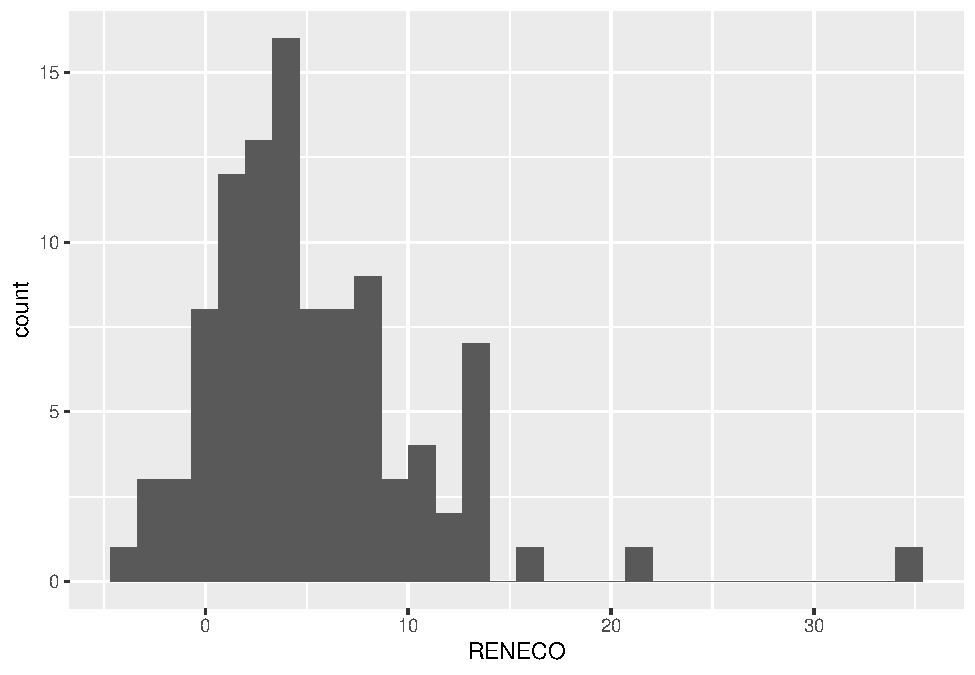
\includegraphics{_main_files/figure-latex/unnamed-chunk-107-1.pdf}

Por supuesto, \texttt{\{ggplot2\}} permite personalizar y refinar la apariencia del gráfico. Uno de los aspectos que nos puede interesar modificar es el número de intervalos en los que queda dividido el rango de valores que puede tomar la variable (``grosor'' de las barras), o \emph{bins}. Por defecto, el número es 30. Para incrementar este número de barras a 40, por ejemplo, añadiremos en la línea del \emph{geom} el argumento \textbf{``bins =''}:

\begin{Shaded}
\begin{Highlighting}[]
\CommentTok{\#Histograma}
\FunctionTok{ggplot}\NormalTok{(}\AttributeTok{data =}\NormalTok{ eolica\_100, }\AttributeTok{map =} \FunctionTok{aes}\NormalTok{(}\AttributeTok{x =}\NormalTok{ RENECO)) }\SpecialCharTok{+}
       \FunctionTok{geom\_histogram}\NormalTok{(}\AttributeTok{bins =} \DecValTok{40}\NormalTok{)}
\end{Highlighting}
\end{Shaded}

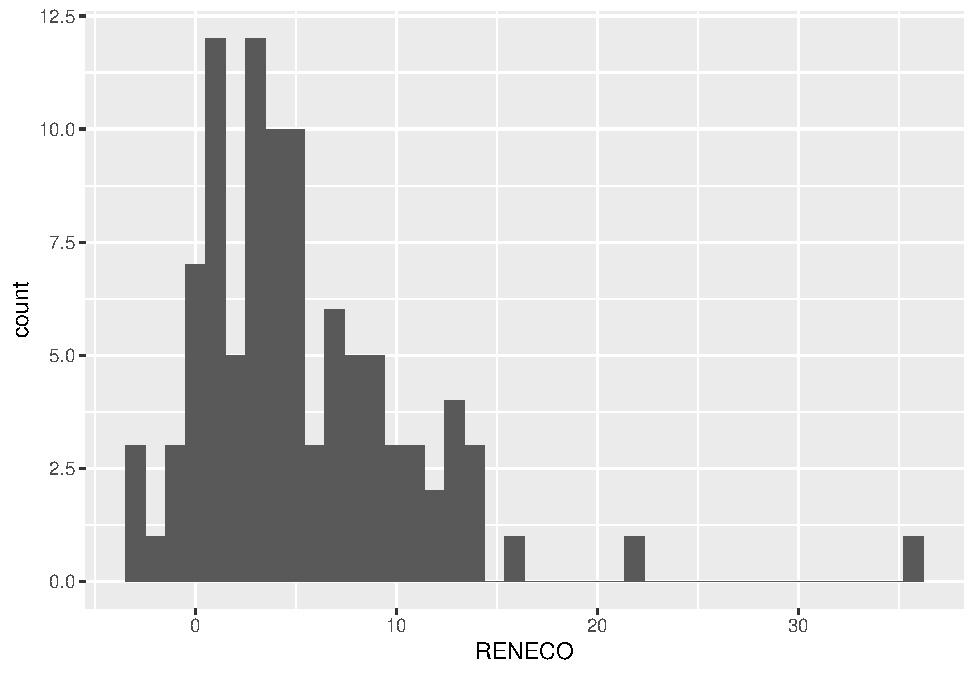
\includegraphics{_main_files/figure-latex/unnamed-chunk-108-1.pdf}

A continuación, vamos a modificar el color de las barras. Para el borde de estas, se utiliza el argumento \textbf{``colour =''}; y, para el relleno, \textbf{``fill =''}. Además, vamos a mejorar la presentación del gráfico añadiéndole un título y un subtítulo, y unas etiquetas en los ejes. Hay que prestar atención a los signos \textbf{``+''} incluidos para que R entienda que el código de la siguiente línea pertenece al mismo gráfico que estamos diseñando:

\begin{Shaded}
\begin{Highlighting}[]
\FunctionTok{ggplot}\NormalTok{(}\AttributeTok{data =}\NormalTok{ eolica\_100, }\AttributeTok{map =} \FunctionTok{aes}\NormalTok{(}\AttributeTok{x =}\NormalTok{ RENECO)) }\SpecialCharTok{+}
  \FunctionTok{geom\_histogram}\NormalTok{(}\AttributeTok{bins =} \DecValTok{40}\NormalTok{, }\AttributeTok{colour =} \StringTok{"red"}\NormalTok{, }\AttributeTok{fill =} \StringTok{"orange"}\NormalTok{) }\SpecialCharTok{+}
  \FunctionTok{ggtitle}\NormalTok{(}\StringTok{"RENTABILIDAD ECONÓMICA"}\NormalTok{, }\AttributeTok{subtitle =} \StringTok{"100 empresas eólicas"}\NormalTok{)}\SpecialCharTok{+}
  \FunctionTok{xlab}\NormalTok{(}\StringTok{"Rentabilidad Económica (\%)"}\NormalTok{) }\SpecialCharTok{+}
  \FunctionTok{ylab}\NormalTok{(}\StringTok{"Frecuencias"}\NormalTok{)}
\end{Highlighting}
\end{Shaded}

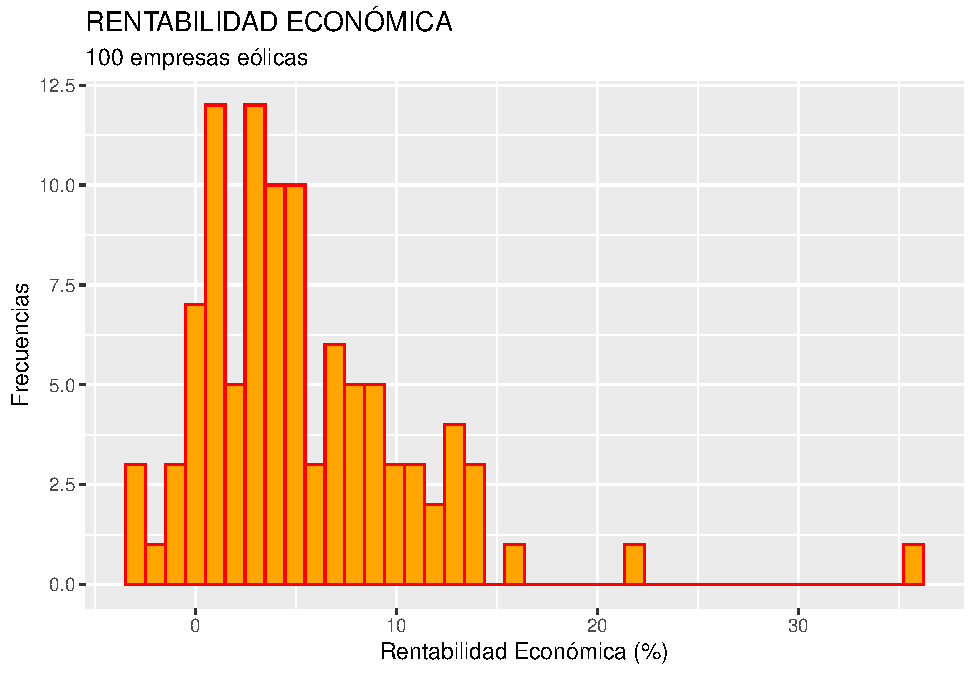
\includegraphics{_main_files/figure-latex/unnamed-chunk-109-1.pdf}

Puede ser que nos interese diferenciar los casos según grupos preestablecidos. Por ejemplo, entre las variables de nuestro \emph{data frame} ``eolica\_100'', existe una variable categórica, atributo o factor, denominada DIMENSION, que clasifica a las 100 empresas en ``GRANDE'', ``MEDIO'' o ``PEQUEÑO'' atendiendo al tamaño del grupo empresarial al que pertenecen (medido en número de empresas). Lo que vamos a hacer es crear, en el mismo gráfico, un histograma de la rentabilidad económica, pero para cada categoría de DIMENSION. Para ello, habrá que incluir esta variable categórica en el ``mapeo'', en concreto mediante el argumento ``fill =''. \textbf{Es} \textbf{necesario hacerlo dentro del elemento \emph{aes}}, ya que el resultado (color de grupo de empresas) depende del valor que toma la variable DIMENSION para cada caso o empresa:

\begin{Shaded}
\begin{Highlighting}[]
\FunctionTok{ggplot}\NormalTok{(}\AttributeTok{data =}\NormalTok{ eolica\_100, }\AttributeTok{map =} \FunctionTok{aes}\NormalTok{(}\AttributeTok{x =}\NormalTok{ RENECO, }\AttributeTok{fill =}\NormalTok{ DIMENSION)) }\SpecialCharTok{+}
  \FunctionTok{geom\_histogram}\NormalTok{(}\AttributeTok{bins =} \DecValTok{60}\NormalTok{, }\AttributeTok{colour =} \StringTok{"red"}\NormalTok{) }\SpecialCharTok{+}
  \FunctionTok{scale\_fill\_brewer}\NormalTok{(}\AttributeTok{palette =} \StringTok{"Oranges"}\NormalTok{) }\SpecialCharTok{+}
  \FunctionTok{ggtitle}\NormalTok{(}\StringTok{"RENTABILIDAD ECONÓMICA"}\NormalTok{, }\AttributeTok{subtitle =} \StringTok{"100 empresas eólicas"}\NormalTok{)}\SpecialCharTok{+}
  \FunctionTok{xlab}\NormalTok{(}\StringTok{"Rentabilidad Económica (\%)"}\NormalTok{) }\SpecialCharTok{+}
  \FunctionTok{ylab}\NormalTok{(}\StringTok{"Frecuencias"}\NormalTok{)}
\end{Highlighting}
\end{Shaded}

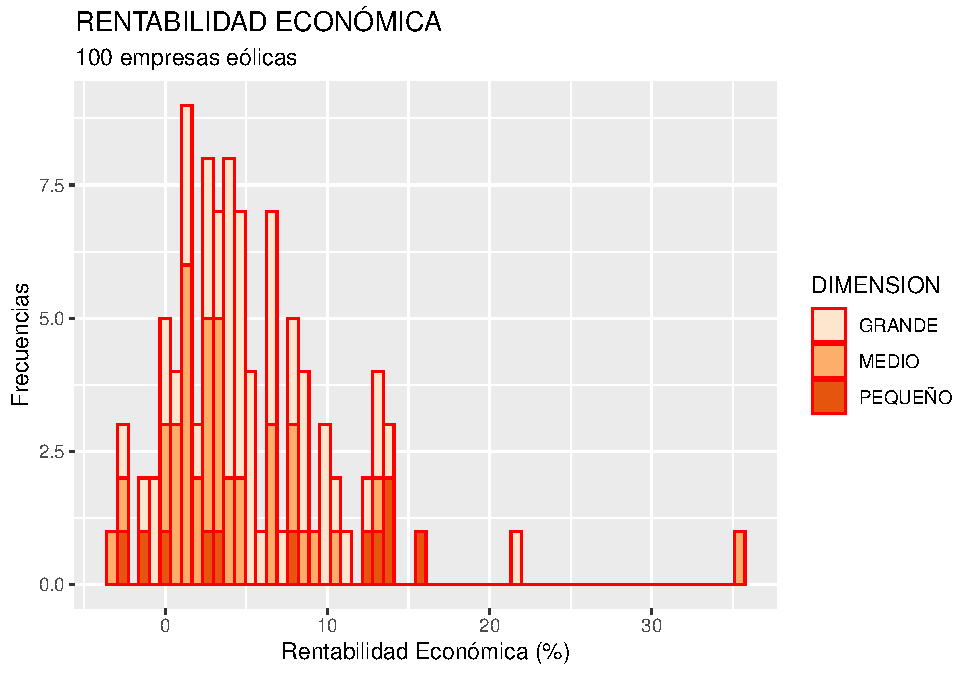
\includegraphics{_main_files/figure-latex/unnamed-chunk-110-1.pdf}

Como puede comprobarse, se superponen los tres histogramas, con tres colores diferentes, dependiendo de la dimensión considerada. Además, aparece, al lado derecho del gráfico, una leyenda que detalla qué color se asocia a cada uno de los grupos de empresas. La función \texttt{scale\_fill\_brewer()} nos permite personalizar la paleta de colores a utilizar (para ver las paletas disponibles, podemos consultar \href{https://ggplot2-book.org/scales-colour}{esta sección} de (\citeproc{ref-ggplot22021}{Wickham 2021}).

\subsection{Gráfico de densidad.}\label{gruxe1fico-de-densidad.}

Un gráfico parecido al histograma es el de \textbf{densidad}. Un gráfico de densidad estima la función de probabilidad empírica de la variable representada. En realidad, podemos considerarlo como un histograma ``suavizado''. Probemos a ejecutar este código:

\begin{Shaded}
\begin{Highlighting}[]
\FunctionTok{ggplot}\NormalTok{(}\AttributeTok{data =}\NormalTok{ eolica\_100, }\AttributeTok{map =} \FunctionTok{aes}\NormalTok{(}\AttributeTok{x =}\NormalTok{ RENECO)) }\SpecialCharTok{+}
  \FunctionTok{geom\_density}\NormalTok{(}\AttributeTok{colour =} \StringTok{"red"}\NormalTok{, }\AttributeTok{fill =} \StringTok{"orange"}\NormalTok{) }\SpecialCharTok{+}
  \FunctionTok{ggtitle}\NormalTok{(}\StringTok{"RENTABILIDAD ECONÓMICA"}\NormalTok{, }\AttributeTok{subtitle =} \StringTok{"100 empresas eólicas"}\NormalTok{)}\SpecialCharTok{+}
  \FunctionTok{xlab}\NormalTok{(}\StringTok{"Rentabilidad Económica (\%)"}\NormalTok{) }\SpecialCharTok{+}
  \FunctionTok{ylab}\NormalTok{(}\StringTok{"Densidad"}\NormalTok{)}
\end{Highlighting}
\end{Shaded}

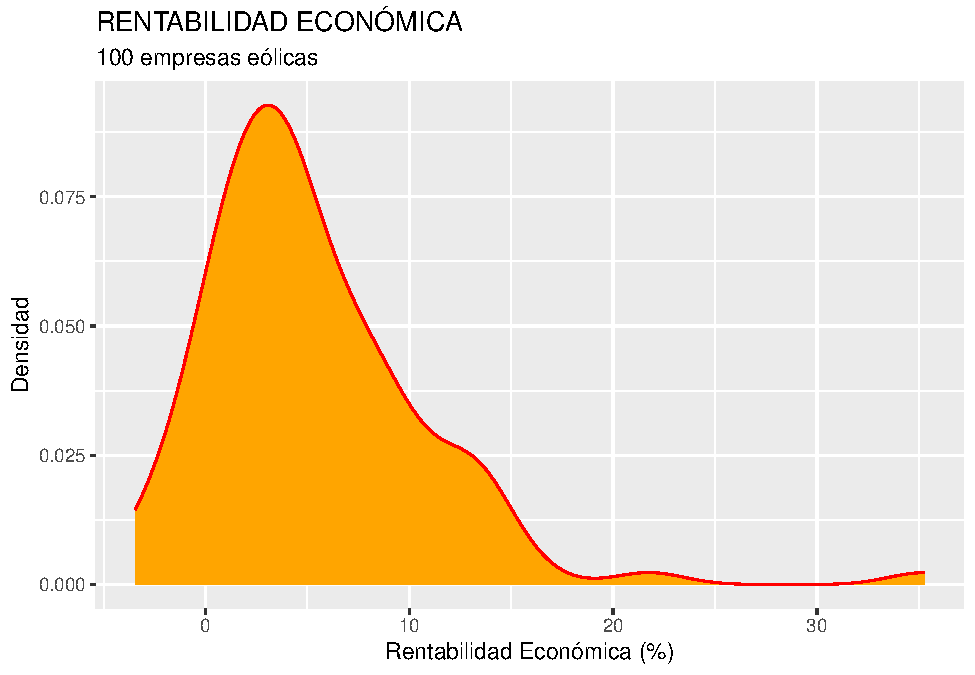
\includegraphics{_main_files/figure-latex/unnamed-chunk-111-1.pdf}

En el código se observa la utilización del tipo de gráfico \texttt{geom\_density()}. Además, desaparece el número de intervalos o \emph{bins}, y se puede dotar a la función de densidad estimada de un color en su borde (\texttt{colour=}), y de un color de relleno (\texttt{fill=}).

Como en casos anteriores, se puede crear una función de densidad estimada para cada grupo de empresas, eliminando las características, \texttt{colour=} y \texttt{fill=} del bloque del \emph{geom}, y añadiéndolas en el ``mapeo'', dentro del \texttt{aes()}:

\begin{Shaded}
\begin{Highlighting}[]
\FunctionTok{ggplot}\NormalTok{(}\AttributeTok{data =}\NormalTok{ eolica\_100, }\AttributeTok{map =} \FunctionTok{aes}\NormalTok{(}\AttributeTok{x =}\NormalTok{ RENECO, }\AttributeTok{fill =}\NormalTok{ DIMENSION)) }\SpecialCharTok{+}
  \FunctionTok{geom\_density}\NormalTok{(}\AttributeTok{colour =} \StringTok{"red"}\NormalTok{, }\AttributeTok{alpha =} \FloatTok{0.70}\NormalTok{, ) }\SpecialCharTok{+}
  \FunctionTok{scale\_fill\_brewer}\NormalTok{(}\AttributeTok{palette =} \StringTok{"Oranges"}\NormalTok{) }\SpecialCharTok{+}
  \FunctionTok{ggtitle}\NormalTok{(}\StringTok{"RENTABILIDAD ECONÓMICA"}\NormalTok{, }\AttributeTok{subtitle =} \StringTok{"100 empresas eólicas"}\NormalTok{)}\SpecialCharTok{+}
  \FunctionTok{xlab}\NormalTok{(}\StringTok{"Rentabilidad Económica (\%)"}\NormalTok{) }\SpecialCharTok{+}
  \FunctionTok{ylab}\NormalTok{(}\StringTok{"Densidad"}\NormalTok{)}
\end{Highlighting}
\end{Shaded}

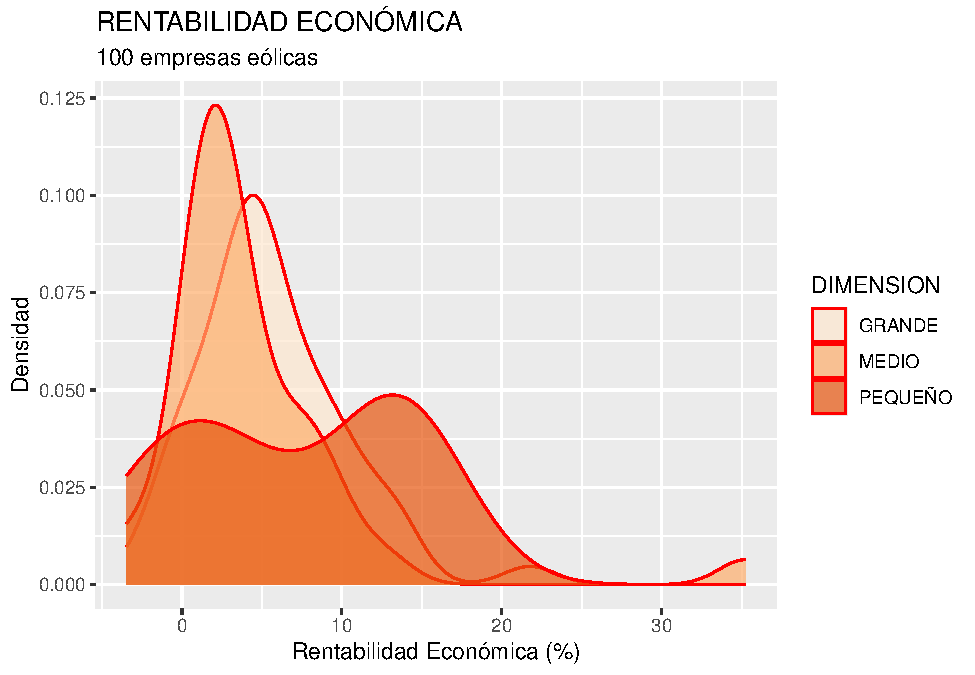
\includegraphics{_main_files/figure-latex/unnamed-chunk-112-1.pdf}

En efecto, el argumento \texttt{fill=} ha pasado a integrarse, en el ``mapeo'', dentro de un elemento \texttt{aes}, ya que el color de relleno va a variar dependiendo del grupo de pertenencia de la empresa (variable DIMENSION). Por otro lado, en el \texttt{geom} se ha añadido el argumento \texttt{alpha=}. Esta información consiste en un número de 0 a 1 que gradúa el grado de transparencia / opacidad de los rellenos de las figuras (en este caso las funciones de densidad estimadas) incluidas en los gráficos.

\subsection{\texorpdfstring{Gráfico de caja o \emph{Box-Plot}.}{Gráfico de caja o Box-Plot.}}\label{gruxe1fico-de-caja-o-box-plot.}

Un tipo muy interesante de gráfico es el de ``caja'' (\textbf{\emph{box-plot}}), que informa de la dispersión de una variable. Fijémonos en el siguiente código:

\begin{Shaded}
\begin{Highlighting}[]
\FunctionTok{ggplot}\NormalTok{(}\AttributeTok{data =}\NormalTok{ eolica\_100, }\AttributeTok{map =}\NormalTok{ (}\FunctionTok{aes}\NormalTok{(}\AttributeTok{y =}\NormalTok{ RENECO))) }\SpecialCharTok{+}
  \FunctionTok{geom\_boxplot}\NormalTok{(}\AttributeTok{fill=} \StringTok{"orange"}\NormalTok{) }\SpecialCharTok{+}
  \FunctionTok{ggtitle}\NormalTok{(}\StringTok{"RENTABILIDAD ECONÓMICA"}\NormalTok{, }\AttributeTok{subtitle =} \StringTok{"100 empresas eólicas"}\NormalTok{) }\SpecialCharTok{+}
  \FunctionTok{ylab}\NormalTok{(}\StringTok{"Rentabilidad Económica (\%)"}\NormalTok{)}
\end{Highlighting}
\end{Shaded}

Puede observarse cómo en el ``mapeo'' se fija la variable que va a determinar las coordenadas del eje ``y''. Como es una variable, hay que incluirla en el ``mapeo'' mediante una característica \texttt{aes}. El \texttt{geom} o tipo de gráfico es \texttt{geom\_boxplot()}, y en este caso no le hemos añadido ninguna característica específica. Las últimas líneas configuran los títulos del gráfico y del eje ``y''. El resultado de ejecutar el código es el siguiente gráfico:

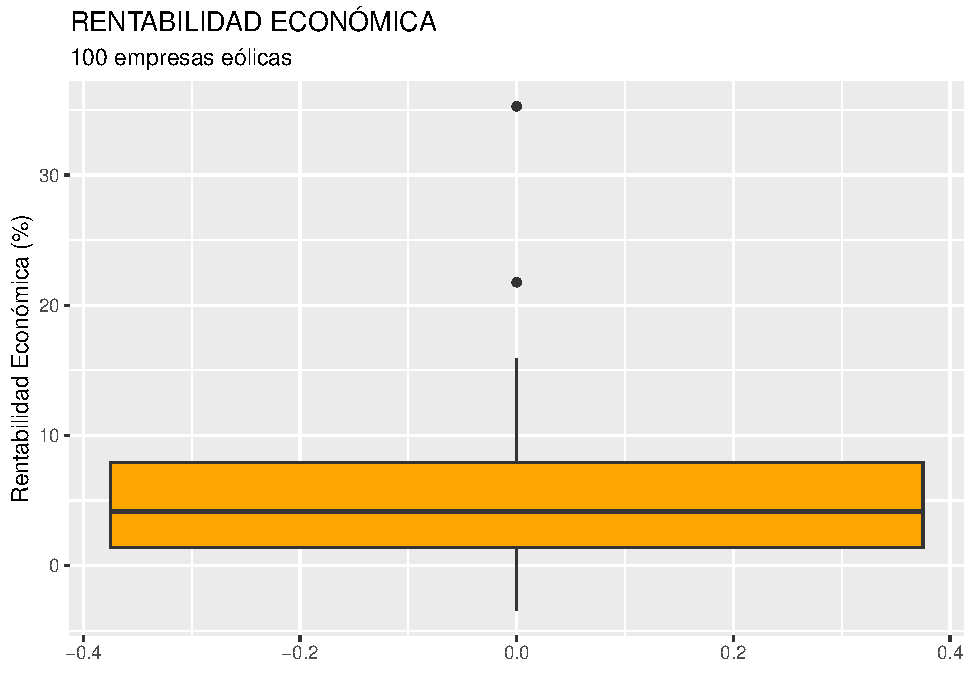
\includegraphics{_main_files/figure-latex/unnamed-chunk-114-1.pdf}

El gráfico se caracteriza por una ``caja'' (rectángulo) central. Esta caja está limitada por el primer y tercer cuartil, luego recoge el 50\% de los casos con una rentabilidad económica superior al 25\% de los casos con menor rentabilidad, y por debajo del 25\% de los casos con la rentabilidad más alta. Así, la altura de la caja es la diferencia entre los cuartiles tercero y primero, que es lo que se denomina ``rango intercuartílico'' (\emph{IQR} por las siglas en inglés). La caja, a su vez, está dividida en dos zonas por una línea horizontal, que es la mediana de la distribución: la rentabilidad económica que divide a los casos en dos grupos con el mismo número de casos, uno con los casos de mayor rentabilidad, y otro con los casos de menor rentabilidad.

Por encima y por debajo de la caja se disponen dos segmentos (llamados ``bigotes''). Estos ``bigotes'' recogen los casos con valores en la variable inferiores al primer cuartil (comenzando por la base de la caja, hacia abajo), o superiores al tercer cuartil (comenzando por el techo de la caja, hacia arriba); y que están a menos de \textbf{1.5 veces} la altura de la caja. Los casos con valores de rentabilidad inferiores al primer cuartil (por abajo) y superiores al tercero (por arriba), que están alejados de la caja en más de 1.5 veces la altura de esta, se indican con puntos, y se corresponden con los casos conocidos como \textbf{casos atípicos} o \textbf{\emph{outliers}}. La identificación de los \emph{outliers} es una fase muy importante a la hora de aplicar algunas técnicas estadísticas.

En esta práctica, comprobamos cómo, en el caso de la rentabilidad económica (RENECO), existen dos \emph{outliers}, es decir, dos casos que presentan sendas rentabilidades anormalmente elevadas (más de un 20\%).

Vamos a refinar el \emph{box-plot} anterior. Por ejemplo, quizá nos pueda interesar crear un \emph{box-plot} para cada grupo de empresas, según el tamaño del grupo empresarial de pertenencia (atributo DIMENSION). Esto lo conseguiremos con el código:

\begin{Shaded}
\begin{Highlighting}[]
\FunctionTok{ggplot}\NormalTok{(}\AttributeTok{data =}\NormalTok{ eolica\_100, }\AttributeTok{map =}\NormalTok{ (}\FunctionTok{aes}\NormalTok{(}\AttributeTok{x =}\NormalTok{ DIMENSION, }\AttributeTok{y =}\NormalTok{ RENECO, }\AttributeTok{fill =}\NormalTok{ DIMENSION))) }\SpecialCharTok{+}
  \FunctionTok{geom\_boxplot}\NormalTok{() }\SpecialCharTok{+}
  \FunctionTok{stat\_summary}\NormalTok{(}\AttributeTok{fun =} \StringTok{"mean"}\NormalTok{,}
               \AttributeTok{geom =} \StringTok{"point"}\NormalTok{,}
               \AttributeTok{size =} \DecValTok{3}\NormalTok{,}
               \AttributeTok{col =} \StringTok{"darkblue"}\NormalTok{) }\SpecialCharTok{+}
  \FunctionTok{stat\_summary}\NormalTok{(}\AttributeTok{fun =} \StringTok{"mean"}\NormalTok{,}
               \AttributeTok{geom =} \StringTok{"line"}\NormalTok{,}
               \AttributeTok{col =} \StringTok{"darkblue"}\NormalTok{,}
               \AttributeTok{map =}\NormalTok{ (}\FunctionTok{aes}\NormalTok{(}\AttributeTok{group =} \ConstantTok{TRUE}\NormalTok{))) }\SpecialCharTok{+}
  \FunctionTok{scale\_fill\_brewer}\NormalTok{(}\AttributeTok{palette =} \StringTok{"Oranges"}\NormalTok{) }\SpecialCharTok{+}
  \FunctionTok{ggtitle}\NormalTok{(}\StringTok{"RENTABILIDAD ECONÓMICA"}\NormalTok{, }\AttributeTok{subtitle =} \StringTok{"100 empresas eólicas"}\NormalTok{) }\SpecialCharTok{+}
  \FunctionTok{ylab}\NormalTok{(}\StringTok{"Rentabilidad Económica (\%)"}\NormalTok{)}
\end{Highlighting}
\end{Shaded}

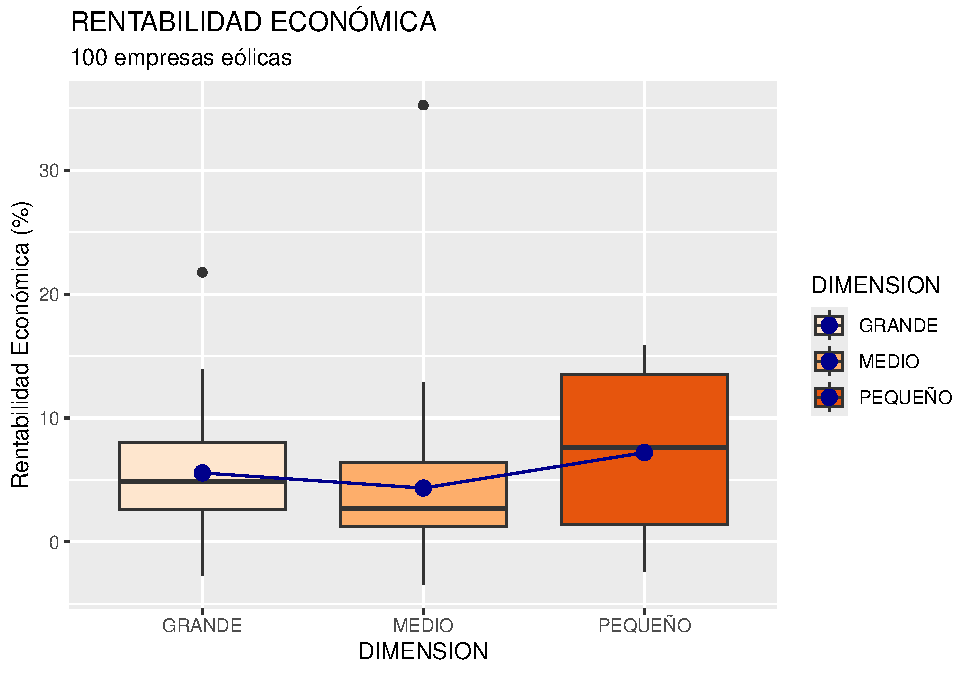
\includegraphics{_main_files/figure-latex/unnamed-chunk-115-1.pdf}

Para construir una caja por categoría de la variable cualitativa o atributo DIMENSION, se ha incluido, en el ``mapeo'' de la primera línea, el eje x con la variable tal variable DIMENSION. Como, además, queremos que cada caja sea de un color diferente, hemos hecho que los colores de estas dependan de la variable DIMENSION; añadiendo en el \texttt{aes()} del ``mapeo'' la característica \texttt{fill=} (que se refiere al color de relleno de las cajas).

Dentro de las cajas, se representan las medianas de la variable estudiada (RENECO), para cada grupo de empresas. Pero, a veces, es muy útil representar también otra medida de posición central como es la \textbf{media}. En los gráficos diseñados con \texttt{\{ggplot2\}} se pueden añadir medidas estadísticas mediante elementos \texttt{stat\_summary()}, algo parecido al \texttt{summarise()} de \texttt{\{dplyr\}}. Estos elementos contienen una serie de informaciones, como son \texttt{fun\ =} (la función, medida, o estadístico a representar), un \texttt{geom} (tipo de gráfico), y otros elementos opcionales. En el ejemplo, el primer bloque de \texttt{stat\_summary()} consigue puntear, para cada grupo de empresas, la media de RENECO en dicho grupo, en color azul oscuro. Para comparar mejor estas medias, se ha procedido a unir los puntos con unos segmentos o líneas de color azul oscuro, lo que se consigue con el segundo bloque de \texttt{stat\_summary()}. La última línea de ese bloque, \texttt{map\ =\ (aes(group\ =\ TRUE)))}, obliga a que las líneas vayan de una media a otra de los grupos (de punto azul oscuro a punto azul oscuro).

Como última extensión, se ha considerado que, a veces, es conveniente tener en cuenta la posición de cada caso individual dentro del gráfico. Una opción es utilizar una capa o bloque \texttt{geom\_jitter()}. Con este \texttt{geom} se dispondrán, para cada grupo, los valores individuales de la variable RENECO; y para que estos, en su caso, no se solapen, se situarán un poco más a la izquierda o a la derecha, de modo aleatorio. Como los \emph{outliers} son ya casos individuales, para que no se dupliquen con los provenientes del ``jitter'', se indicará en el \texttt{geom\_boxplot()} que, en ese bloque gráfico, no se señalen los \emph{outliers}. Esto se conseguirá con el argumento \texttt{outlier.shape\ =\ NA}. El código, en definitiva, será:

\begin{Shaded}
\begin{Highlighting}[]
\FunctionTok{ggplot}\NormalTok{(}\AttributeTok{data =}\NormalTok{ eolica\_100, }\AttributeTok{map =}\NormalTok{ (}\FunctionTok{aes}\NormalTok{(}\AttributeTok{x =}\NormalTok{ DIMENSION, }\AttributeTok{y =}\NormalTok{ RENECO, }\AttributeTok{fill =}\NormalTok{ DIMENSION))) }\SpecialCharTok{+}
  \FunctionTok{geom\_boxplot}\NormalTok{(}\AttributeTok{outlier.shape =} \ConstantTok{NA}\NormalTok{) }\SpecialCharTok{+}
  \FunctionTok{stat\_summary}\NormalTok{(}\AttributeTok{fun =} \StringTok{"mean"}\NormalTok{,}
               \AttributeTok{geom =} \StringTok{"point"}\NormalTok{,}
               \AttributeTok{size =} \DecValTok{3}\NormalTok{,}
               \AttributeTok{col =} \StringTok{"darkblue"}\NormalTok{) }\SpecialCharTok{+}
  \FunctionTok{stat\_summary}\NormalTok{(}\AttributeTok{fun =} \StringTok{"mean"}\NormalTok{,}
               \AttributeTok{geom =} \StringTok{"line"}\NormalTok{,}
               \AttributeTok{col =} \StringTok{"darkblue"}\NormalTok{,}
               \AttributeTok{map =}\NormalTok{ (}\FunctionTok{aes}\NormalTok{(}\AttributeTok{group =} \ConstantTok{TRUE}\NormalTok{))) }\SpecialCharTok{+}
    \FunctionTok{geom\_jitter}\NormalTok{(}\AttributeTok{width =} \FloatTok{0.1}\NormalTok{,}
              \AttributeTok{size =} \DecValTok{1}\NormalTok{,}
              \AttributeTok{col =} \StringTok{"darkred"}\NormalTok{,}
              \AttributeTok{alpha =} \FloatTok{0.40}\NormalTok{) }\SpecialCharTok{+}

  \FunctionTok{scale\_fill\_brewer}\NormalTok{(}\AttributeTok{palette =} \StringTok{"Oranges"}\NormalTok{) }\SpecialCharTok{+}
  \FunctionTok{ggtitle}\NormalTok{(}\StringTok{"RENTABILIDAD ECONÓMICA"}\NormalTok{, }\AttributeTok{subtitle =} \StringTok{"100 empresas eólicas"}\NormalTok{) }\SpecialCharTok{+}
  \FunctionTok{ylab}\NormalTok{(}\StringTok{"Rentabilidad Económica (\%)"}\NormalTok{)}
\end{Highlighting}
\end{Shaded}

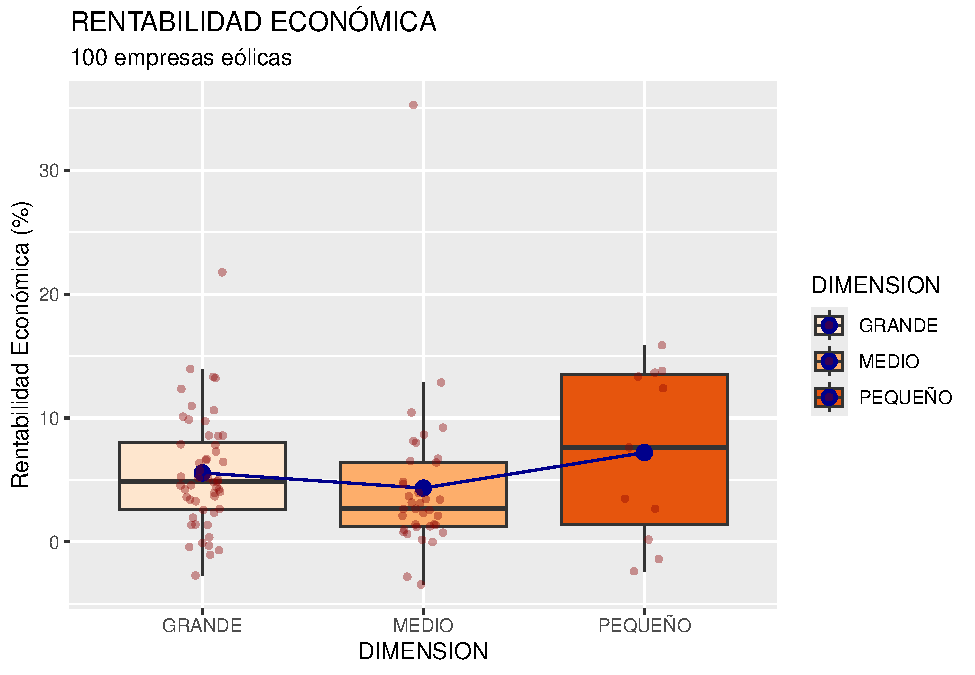
\includegraphics{_main_files/figure-latex/unnamed-chunk-116-1.pdf}

Como puede observarse, el \texttt{geom\_jitter()} proporciona, en cada caja, la nube de casos (empresas) individuales, en cuanto a la rentabilidad económica (incluidos los \emph{outliers}). Las características de estos puntos (amplitud del desplazamiento lateral ``aleatorio'', tamaño, color, opacidad) se controlan con diversos argumentos (\texttt{width=}, \texttt{size=}, \texttt{col=}, \texttt{alpha=}).

\section{Gráficos de dos variables.}\label{gruxe1ficos-de-dos-variables.}

\subsection{\texorpdfstring{Gráfico de dispersión o \emph{scatterplot}.}{Gráfico de dispersión o scatterplot.}}\label{gruxe1fico-de-dispersiuxf3n-o-scatterplot.}

Pasamos ahora a comentar un tipo de gráfico muy común cuando trabajamos con dos variables métricas: los \textbf{gráficos de dispersión} (o \textbf{\emph{scatterplots}}). En este tipo de gráficos, cada variable ocupa un eje (x o y), y los puntos internos al gráfico representan los diversos casos u observaciones.

Como ejemplo, vamos a crear un gráfico de dispersión que represente las empresas eólicas en función de su rentabilidad económica (RENECO) y de su rentabilidad financiera (RENFIN). El código es el siguiente:

\begin{Shaded}
\begin{Highlighting}[]
\FunctionTok{ggplot}\NormalTok{(}\AttributeTok{data =}\NormalTok{ eolica\_100, }\AttributeTok{map =}\NormalTok{ (}\FunctionTok{aes}\NormalTok{(}\AttributeTok{x =}\NormalTok{ RENECO, }\AttributeTok{y =}\NormalTok{ RENFIN))) }\SpecialCharTok{+}
  \FunctionTok{geom\_point}\NormalTok{(}\AttributeTok{color =} \StringTok{"red"}\NormalTok{, }\AttributeTok{size =} \DecValTok{2}\NormalTok{, }\AttributeTok{alpha =} \FloatTok{0.7}\NormalTok{) }\SpecialCharTok{+}
  \FunctionTok{ggtitle}\NormalTok{(}\StringTok{"RENTABILIDAD ECONÓMICA vs RENTABILIDAD FINANCIERA"}\NormalTok{, }\AttributeTok{subtitle =} \StringTok{"100 empresas eólicas"}\NormalTok{) }\SpecialCharTok{+}
  \FunctionTok{xlab}\NormalTok{(}\StringTok{"Rentabilidad Económica (\%)"}\NormalTok{) }\SpecialCharTok{+}
  \FunctionTok{ylab}\NormalTok{(}\StringTok{"Rentabilidad Financiera (\%)"}\NormalTok{)}
\end{Highlighting}
\end{Shaded}

El resultado es el siguiente gráfico:

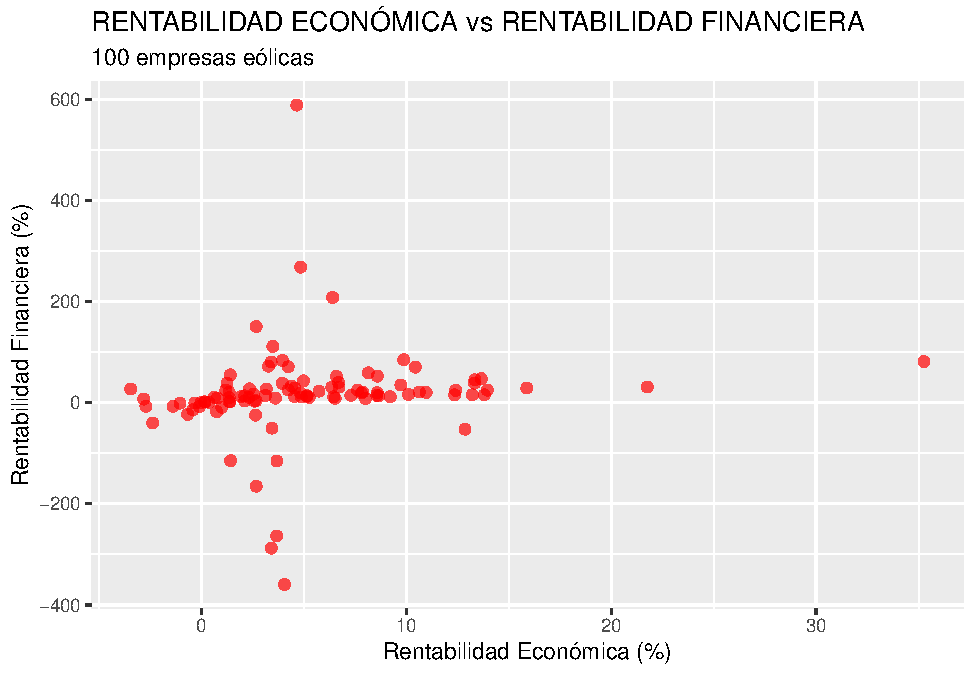
\includegraphics{_main_files/figure-latex/unnamed-chunk-118-1.pdf}

Vamos a refinar el gráfico algo más. En primer lugar, puede ser interesante \textbf{distinguir entre los tipos de empresas}, según el tamaño del grupo empresarial al que pertenecen ( variable DIMENSION). Para ello, podemos poner el color de los puntos en el ``mapeo'', en función de la variable DIMENSION:

\begin{Shaded}
\begin{Highlighting}[]
\FunctionTok{ggplot}\NormalTok{(}\AttributeTok{data =}\NormalTok{ eolica\_100, }\AttributeTok{map =}\NormalTok{ (}\FunctionTok{aes}\NormalTok{(}\AttributeTok{x =}\NormalTok{ RENECO,}
                                     \AttributeTok{y =}\NormalTok{ RENFIN,}
                                     \AttributeTok{col =}\NormalTok{ DIMENSION))) }\SpecialCharTok{+}
  \FunctionTok{geom\_point}\NormalTok{(}\AttributeTok{size =} \DecValTok{2}\NormalTok{, }\AttributeTok{alpha =} \FloatTok{0.7}\NormalTok{) }\SpecialCharTok{+}
  \FunctionTok{ggtitle}\NormalTok{(}\StringTok{"RENTABILIDAD ECONÓMICA vs FINANCIERA"}\NormalTok{,}
          \AttributeTok{subtitle =} \StringTok{"100 empresas eólicas"}\NormalTok{) }\SpecialCharTok{+}
  \FunctionTok{xlab}\NormalTok{(}\StringTok{"Rentabilidad Económica (\%)"}\NormalTok{) }\SpecialCharTok{+}
  \FunctionTok{ylab}\NormalTok{(}\StringTok{"Rentabilidad Financiera (\%)"}\NormalTok{)}
\end{Highlighting}
\end{Shaded}

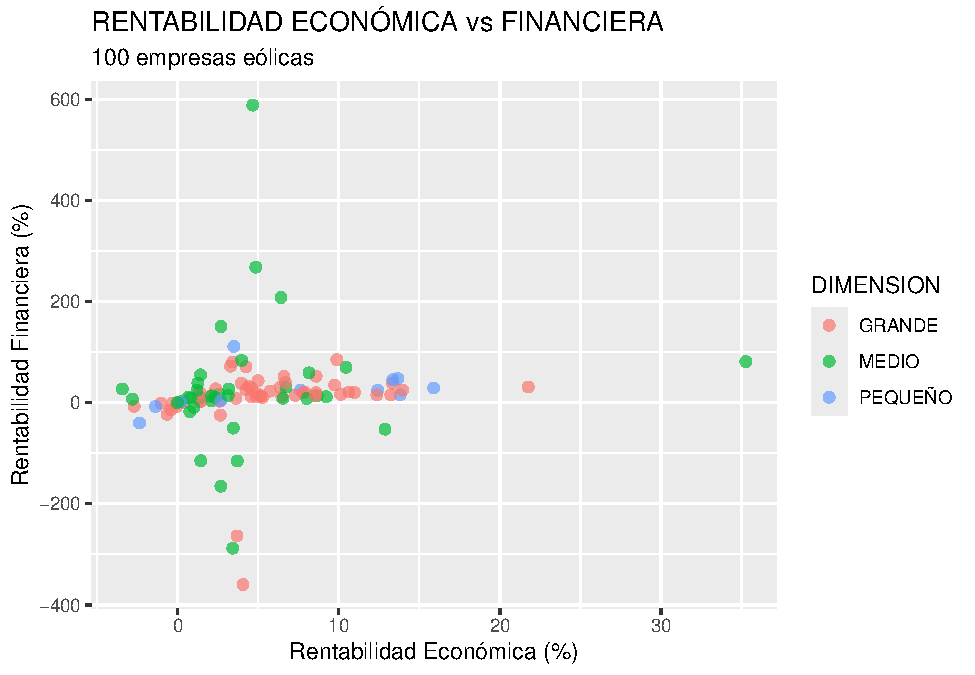
\includegraphics{_main_files/figure-latex/unnamed-chunk-119-1.pdf}

En los dos gráficos anteriores pueden observarse puntos (casos) candidatos a ser \emph{outliers} para cada una de las dos variables analizadas. En el caso de RENECO, ya se pudo advertir esta circunstancia al construir los \emph{boxplots}.

Por otro lado, podría ser interesante complementar el gráfico con información sobre las dos variables por separado, es decir, con \textbf{información sobre las distribuciones marginales}. Existe un paquete complementario a \texttt{\{ggplot2\}}, llamado \texttt{\{ggExtra\}}, que puede ayudar fácilmente a este cometido. Para ello, hemos de activar dicho paquete con \texttt{library()} (si no ha sido previamente instalado, habrá que hacerlo con anterioridad). El segundo paso consistirá en \textbf{asignar} nuestro \emph{scatterplot}, diseñado con la función \texttt{ggplot()}, a un objeto con el nombre que queramos, por ejemplo, ``scatter\_plus''. Luego, ese objeto, que contiene nuestro gráfico, entrará como argumento en la función de \texttt{\{ggExtra\}} llamada \texttt{ggMarginal()}, como se muestra en el siguiente código:

\begin{Shaded}
\begin{Highlighting}[]
\FunctionTok{library}\NormalTok{ (}\StringTok{"ggExtra"}\NormalTok{)}
\NormalTok{scatter\_plus }\OtherTok{\textless{}{-}} \FunctionTok{ggplot}\NormalTok{(}\AttributeTok{data =}\NormalTok{ eolica\_100, }\AttributeTok{map =}\NormalTok{ (}\FunctionTok{aes}\NormalTok{(}\AttributeTok{x =}\NormalTok{ RENECO,}
                                                     \AttributeTok{y =}\NormalTok{ RENFIN,}
                                                     \AttributeTok{col =}\NormalTok{ DIMENSION))) }\SpecialCharTok{+}
  \FunctionTok{geom\_point}\NormalTok{(}\AttributeTok{size =} \DecValTok{2}\NormalTok{, }\AttributeTok{alpha =} \FloatTok{0.7}\NormalTok{) }\SpecialCharTok{+}
  \FunctionTok{ggtitle}\NormalTok{(}\StringTok{"RENTABILIDAD ECONÓMICA vs FINANCIERA"}\NormalTok{,}
          \AttributeTok{subtitle =} \StringTok{"100 empresas eólicas"}\NormalTok{) }\SpecialCharTok{+}
  \FunctionTok{xlab}\NormalTok{(}\StringTok{"Rentabilidad Económica (\%)"}\NormalTok{) }\SpecialCharTok{+}
  \FunctionTok{ylab}\NormalTok{(}\StringTok{"Rentabilidad Financiera (\%)"}\NormalTok{)}
\FunctionTok{ggMarginal}\NormalTok{(scatter\_plus, }\AttributeTok{type =} \StringTok{"histogram"}\NormalTok{, }\AttributeTok{groupColour =}\NormalTok{ T,}
           \AttributeTok{groupFill =}\NormalTok{ T, }\AttributeTok{position =} \StringTok{"identity"}\NormalTok{, }\AttributeTok{alpha =} \FloatTok{0.5}\NormalTok{)}
\end{Highlighting}
\end{Shaded}

Con el código anterior, apreciamos cómo se añaden los histogramas de cada variable, RENECO y RENFIN, en los márgenes del gráfico:

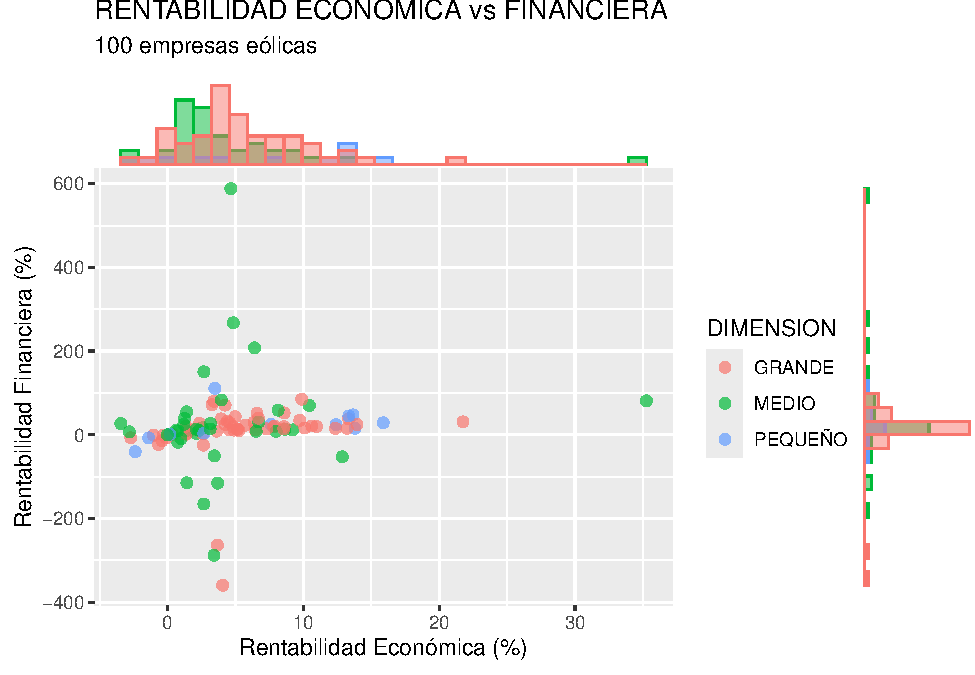
\includegraphics{_main_files/figure-latex/unnamed-chunk-121-1.pdf}

Conviene apuntar que el argumento position = ``identity'' hace que las barras del histograma estén perfectamente alineadas con los datos del gráfico de dispersión, sin ningún tipo de desplazamiento.

Adicionalmente, los diámetros de los puntos de los diversos casos podrían contener también información, haciéndolos proporcionales a una tercera variable. Por ejemplo, podrían ser proporcionales al nivel de solvencia (variable SOLVENCIA). Para ello, ejecutaríamos el código:

\begin{Shaded}
\begin{Highlighting}[]
\NormalTok{scatter\_plus }\OtherTok{\textless{}{-}} \FunctionTok{ggplot}\NormalTok{(}\AttributeTok{data =}\NormalTok{ eolica\_100, }\AttributeTok{map =}\NormalTok{ (}\FunctionTok{aes}\NormalTok{(}\AttributeTok{x =}\NormalTok{ RENECO,}
                                                     \AttributeTok{y =}\NormalTok{ RENFIN,}
                                                     \AttributeTok{col =}\NormalTok{ DIMENSION,}
                                                     \AttributeTok{size =}\NormalTok{ SOLVENCIA))) }\SpecialCharTok{+}
  \FunctionTok{geom\_point}\NormalTok{(}\AttributeTok{alpha =} \FloatTok{0.7}\NormalTok{) }\SpecialCharTok{+}
  \FunctionTok{ggtitle}\NormalTok{(}\StringTok{"RENTABILIDAD ECONÓMICA vs FINANCIERA"}\NormalTok{,}
          \AttributeTok{subtitle =} \StringTok{"100 empresas eólicas"}\NormalTok{) }\SpecialCharTok{+}
  \FunctionTok{xlab}\NormalTok{(}\StringTok{"Rentabilidad Económica (\%)"}\NormalTok{) }\SpecialCharTok{+}
  \FunctionTok{ylab}\NormalTok{(}\StringTok{"Rentabilidad Financiera (\%)"}\NormalTok{)}
\FunctionTok{ggMarginal}\NormalTok{(scatter\_plus, }\AttributeTok{type =} \StringTok{"histogram"}\NormalTok{, }\AttributeTok{groupColour =}\NormalTok{ T,}
           \AttributeTok{groupFill =}\NormalTok{ T, }\AttributeTok{position =} \StringTok{"identity"}\NormalTok{, }\AttributeTok{alpha =} \FloatTok{0.5}\NormalTok{)}
\end{Highlighting}
\end{Shaded}

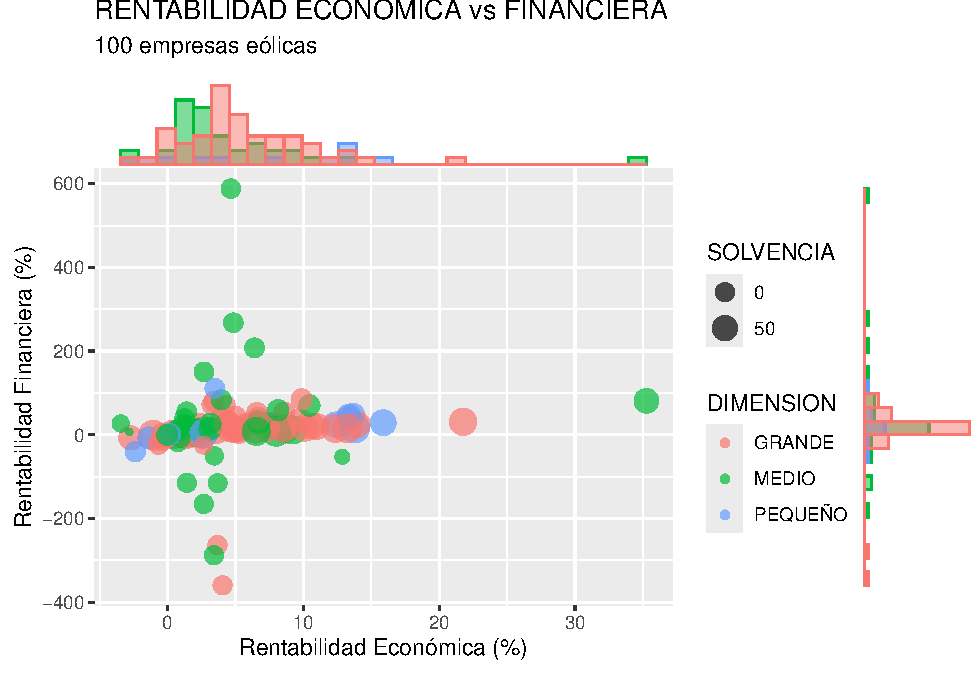
\includegraphics{_main_files/figure-latex/unnamed-chunk-122-1.pdf}

En el código anterior, puede comprobarse que la característica \texttt{size\ =} sube del bloque de \texttt{geom} al ``mapeo'' (incluido en el \texttt{aes}), debido a que el diámetro de cada punto ya no va a ser un parámetro fijo, sino que va a depender de la magnitud de la variable SOLVENCIA.

Finalmente, podría ser útil, en algunos gráficos, añadir una etiqueta (\emph{label}) a cada punto, para \textbf{identificar el caso concreto} al que representa. Si bien en esta práctica, el elevado número de casos y el extenso nombre de las empresas hacen poco claro el uso de estas etiquetas, vamos a añadirlas por motivos pedagógicos. Para ello, se añadirá un bloque \texttt{geom} llamado \texttt{geom\_text()}, con una información \texttt{label\ =} que se hace depender de valores que cambian (en concreto, el nombre de los casos, es decir, de las filas del \emph{data frame}), por lo que tendrá que integrarse en una característica \texttt{aes}:

\begin{Shaded}
\begin{Highlighting}[]
\NormalTok{scatter\_plus }\OtherTok{\textless{}{-}} \FunctionTok{ggplot}\NormalTok{(}\AttributeTok{data =}\NormalTok{ eolica\_100, }\AttributeTok{map =}\NormalTok{ (}\FunctionTok{aes}\NormalTok{(}\AttributeTok{x =}\NormalTok{ RENECO,}
                                                     \AttributeTok{y =}\NormalTok{ RENFIN,}
                                                     \AttributeTok{col =}\NormalTok{ DIMENSION,}
                                                     \AttributeTok{size =}\NormalTok{ SOLVENCIA))) }\SpecialCharTok{+}
 \FunctionTok{geom\_point}\NormalTok{(}\AttributeTok{alpha =} \FloatTok{0.7}\NormalTok{) }\SpecialCharTok{+}
  \FunctionTok{geom\_text}\NormalTok{(}\FunctionTok{aes}\NormalTok{(}\AttributeTok{label=}\FunctionTok{row.names}\NormalTok{(eolica\_100)), }\AttributeTok{size=}\DecValTok{2}\NormalTok{, }\AttributeTok{color=}\StringTok{"black"}\NormalTok{, }\AttributeTok{alpha =} \FloatTok{0.7}\NormalTok{) }\SpecialCharTok{+}
  \FunctionTok{ggtitle}\NormalTok{(}\StringTok{"RENTABILIDAD ECONÓMICA vs FINANCIERA"}\NormalTok{,}
          \AttributeTok{subtitle =} \StringTok{"100 empresas eólicas"}\NormalTok{) }\SpecialCharTok{+}
  \FunctionTok{xlab}\NormalTok{(}\StringTok{"Rentabilidad Económica (\%)"}\NormalTok{) }\SpecialCharTok{+}
  \FunctionTok{ylab}\NormalTok{(}\StringTok{"Rentabilidad Financiera (\%)"}\NormalTok{)}
\FunctionTok{ggMarginal}\NormalTok{(scatter\_plus, }\AttributeTok{type =} \StringTok{"histogram"}\NormalTok{, }\AttributeTok{groupColour =}\NormalTok{ T,}
           \AttributeTok{groupFill =}\NormalTok{ T, }\AttributeTok{position =} \StringTok{"identity"}\NormalTok{, }\AttributeTok{alpha =} \FloatTok{0.5}\NormalTok{)}
\end{Highlighting}
\end{Shaded}

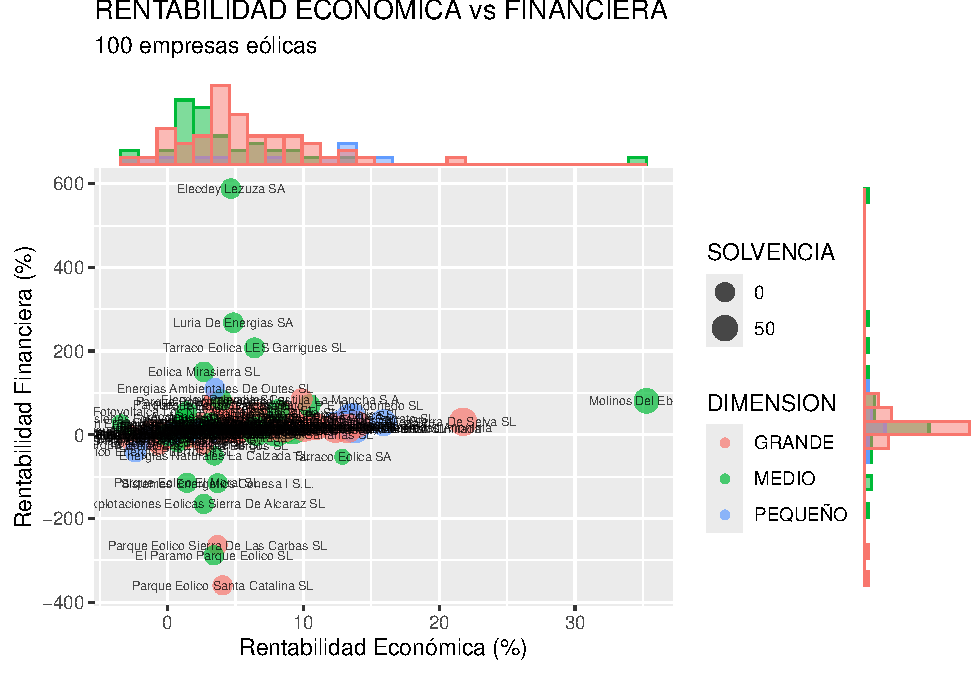
\includegraphics{_main_files/figure-latex/unnamed-chunk-123-1.pdf}

Las etiquetas de los casos pueden refinarse algo más mediante la función \texttt{geom\_label\_repel()}, disponible al cargar el paquete \texttt{\{ggrepel\}}:

\begin{Shaded}
\begin{Highlighting}[]
\FunctionTok{library}\NormalTok{(ggrepel)}
\NormalTok{scatter\_plus }\OtherTok{\textless{}{-}} \FunctionTok{ggplot}\NormalTok{(}\AttributeTok{data =}\NormalTok{ eolica\_100, }\AttributeTok{map =}\NormalTok{ (}\FunctionTok{aes}\NormalTok{(}\AttributeTok{x =}\NormalTok{ RENECO,}
                                                     \AttributeTok{y =}\NormalTok{ RENFIN,}
                                                     \AttributeTok{col =}\NormalTok{ DIMENSION,}
                                                     \AttributeTok{size =}\NormalTok{ SOLVENCIA))) }\SpecialCharTok{+}
  \FunctionTok{geom\_point}\NormalTok{(}\AttributeTok{alpha =} \FloatTok{0.7}\NormalTok{) }\SpecialCharTok{+}
  \FunctionTok{geom\_label\_repel}\NormalTok{(}\FunctionTok{aes}\NormalTok{(}\AttributeTok{label =} \FunctionTok{row.names}\NormalTok{(eolica\_100)),}
                   \AttributeTok{size =} \DecValTok{2}\NormalTok{,}
                   \AttributeTok{color =} \StringTok{"black"}\NormalTok{,}
                   \AttributeTok{alpha =} \FloatTok{0.5}\NormalTok{) }\SpecialCharTok{+}
  \FunctionTok{ggtitle}\NormalTok{(}\StringTok{"RENTABILIDAD ECONÓMICA vs FINANCIERA"}\NormalTok{,}
          \AttributeTok{subtitle =} \StringTok{"100 empresas eólicas"}\NormalTok{) }\SpecialCharTok{+}
  \FunctionTok{xlab}\NormalTok{(}\StringTok{"Rentabilidad Económica (\%)"}\NormalTok{) }\SpecialCharTok{+}
  \FunctionTok{ylab}\NormalTok{(}\StringTok{"Rentabilidad Financiera (\%)"}\NormalTok{)}
\FunctionTok{ggMarginal}\NormalTok{(scatter\_plus, }\AttributeTok{type =} \StringTok{"histogram"}\NormalTok{, }\AttributeTok{groupColour =}\NormalTok{ T,}
           \AttributeTok{groupFill =}\NormalTok{ T,}
           \AttributeTok{position =} \StringTok{"identity"}\NormalTok{, }\AttributeTok{alpha =} \FloatTok{0.5}\NormalTok{)}
\end{Highlighting}
\end{Shaded}

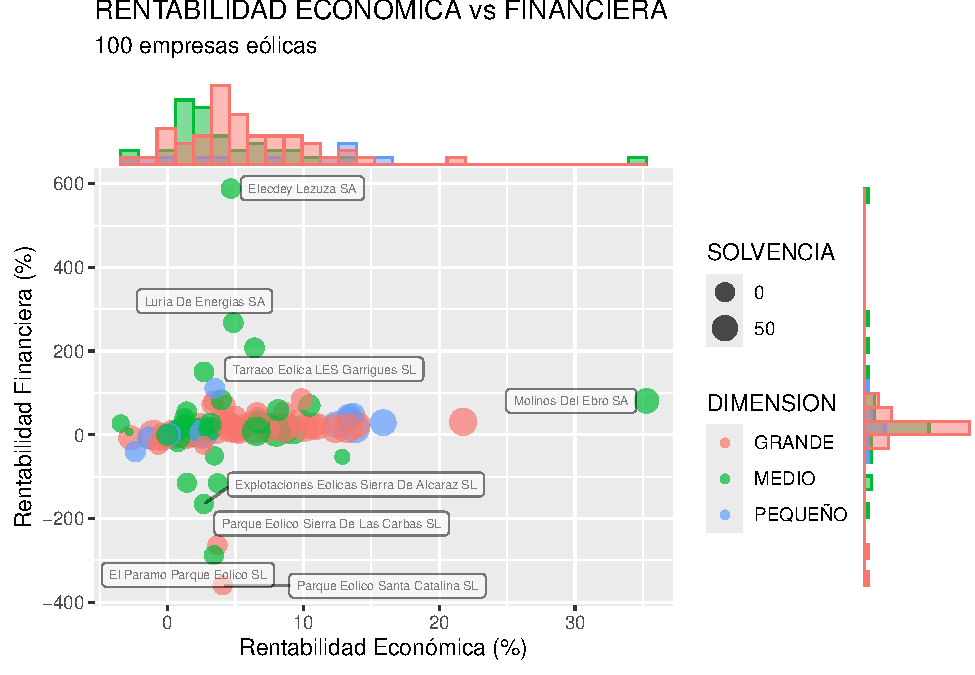
\includegraphics{_main_files/figure-latex/unnamed-chunk-124-1.pdf}

La ventaja de este gráfico, como se puede apreciar, es que se omiten las etiquetas superpuestas, si bien existe el riesgo de que se omitan una gran cantidad de estas.

\section{Materiales para realizar las prácticas del capítulo.}\label{materiales-para-realizar-las-pruxe1cticas-del-capuxedtulo.-1}

En esta sección se muestran los links de acceso a los diferentes materiales (scripts, datos\ldots) necesarios para llevar a cabo los contenidos prácticos del capítulo.

\textbf{Datos (en formato Microsoft (R) Excel (R)):}

\begin{itemize}
\tightlist
\item
  eolica\_100.xlsx (\href{https://docs.google.com/spreadsheets/d/1Up5ZWR57rgIkmYJcr2Pek6kUdG_yd4vu/edit?usp=drive_link&ouid=115375878280465826079&rtpof=true&sd=true}{obtener aquí})
\end{itemize}

\textbf{Scripts:}

\begin{itemize}
\tightlist
\item
  explora\_ggplot2.R (\href{https://drive.google.com/file/d/1Is4XOd6EmFswB6w2eZfC8_pp2mtu7aQK/view?usp=drive_link}{obtener aquí})
\end{itemize}

\chapter{Estadística descriptiva.}\label{estaduxedstica-descriptiva.}

La Estadística Descriptiva es la parte de la Ciencia Estadística que se ocupa de la recopilación de datos, su depuración, y la caracterización mediante dichos datos de un conjunto de casos o individuos.

Los datos se organizan en variables y/o atributos.

Las \textbf{variables} son características de los casos o individuos en estudio que se plasman en valores que están expresados en \textbf{escala métrica}.
Los \textbf{atributos} son características de los casos o individuos en estudio que se concretan en diversas categorías (si el atributo tiene \textbf{escala nominal}) o niveles (si el atributo tiene \textbf{escala ordinal}).
Los atributos se denominan también variables cualitativas o factores.

Centrándonos en las variables (características que afectan a un grupo de casos o individuos, y que se concretan en valores que poseen una escala métrica), podemos plantearnos el estudio de una única variable sin tener en cuenta la existencia de otras variables que caracterizan al mismo grupo de casos o individuos.
En tal caso estaremos planteando un \textbf{análisis estadístico univariante}.
Si nuestro análisis se centra en cómo dos variables caracterizan al mismo conjunto de individuos o casos, y la posible relación entre ambas, estaremos planteando un análisis bivariante.
Generalizando, si estudiamos cómo un grupo de variables caracterizan de modo conjunto a un mismo grupo de casos o individuos, estaremos planteando un \textbf{análisis estadístico multivariante}.

\section{Análisis univariante.}\label{anuxe1lisis-univariante.}

En el análisis estadístico univariante, estudiamos cómo una única característica (nos centraremos en una variable, aunque también puede tratarse de un atributo) afecta a un grupo de casos, individuos o elementos.
Por ejemplo, la variable podría ser el salario percibido por un grupo de individuos que podría ser el conjunto de trabajadores en nómina en una empresa.
Otro ejemplo podría ser el de la (variable) rentabilidad económica obtenida por un grupo de empresas pertenecientes a un determinado sector económico.

El conjunto de pares formado por cada valor que puede tomar la variable en estudio (o categoría o nivel, en el caso de un atributo) y el número de casos que toman tal valor se denomina \textbf{distribución de frecuencias} de la variable.

¿Cómo podemos estudiar el modo en que afecta una variable, de modo global, a un grupo de casos?
Mediante el cálculo de una serie de \textbf{medidas}.
Las medidas son instrumentos matemáticos que extraen y sintetizan la información contenida en una distribución de frecuencias.

Hay diferentes tipos de medidas, principalmente las de \textbf{posición}, \textbf{dispersión} y \textbf{forma}.

Antes de profundizar en las principales medidas, su significado y su obtención; vamos a indicar cómo se pueden presentar en R, mediante la creación de tablas, los datos referentes a un grupo de individuos y las variables o atributos que los caracterizan, y las distribuciones de frecuencias univariantes.

\section{Representando datos y distribuciones de frecuencias en tablas con R.}\label{representando-datos-y-distribuciones-de-frecuencias-en-tablas-con-r.}

Para aprender a representar los datos referentes a las variables y atributos que caracterizan a un grupo de casos o individuos, y las distribuciones de frecuencias univariantes, vamos a suponer que trabajamos dentro de un proyecto que hemos creado previamente, de nombre ``explora''.
Dentro de la carpeta del proyecto guardaremos el \emph{script} llamado ``\href{https://drive.google.com/file/d/1pfyGPGQRmgOyo9wrZ7fr_KAFj49ecXID/view?usp=sharing}{explora\_trabajadores.R}'' y el archivo de \emph{Microsoft® Excel®} llamado ``\href{https://docs.google.com/spreadsheets/d/1e_h8P_0sBuD5Nvw6nkeWtXXeiqItFfdI/edit?usp=sharing&ouid=115375878280465826079&rtpof=true&sd=true}{trabajadores.xlsx}''.

Las primeras líneas del script se refieren, como ya hemos visto en otras secciones del libro, a la limpieza de la memoria o environment, eliminando objetos que se hayan podido crear con anterioridad, y en la importación de los datos que hay en la hoja ``Datos'' de ``trabajadores.xlsx''.
Estos datos se almacenan en el \emph{data frame} ``datos'', y consisten en el registro del salario (variable SALARIO, expresada en cientos de euros), el nivel de estudios (atributo NESTUDIOS) y departamento al que se pertenece (atributo DEP), correspondientes a los 49 trabajadores de una determinada empresa:

\begin{Shaded}
\begin{Highlighting}[]
\CommentTok{\# Script para la construcción de tablas de datos }
\CommentTok{\# y trabajo con distribucionesde frecuencias univariantes.}
\CommentTok{\#}

\FunctionTok{rm}\NormalTok{(}\AttributeTok{list =} \FunctionTok{ls}\NormalTok{())}

\DocumentationTok{\#\# DATOS}

\CommentTok{\# Importando}

\FunctionTok{library}\NormalTok{(readxl)}
\NormalTok{datos }\OtherTok{\textless{}{-}} \FunctionTok{read\_excel}\NormalTok{(}\StringTok{"trabajadores.xlsx"}\NormalTok{, }\AttributeTok{sheet =} \StringTok{"Datos"}\NormalTok{)}
\end{Highlighting}
\end{Shaded}

Como sabemos, R interpreta el nombre de los trabajadores como una variable más, en lugar de como la identificador de cada ``fila'' o caso.
Para corregir esto, y hacer saber a R que la primera columna no es una variable, sino el nombre de cada fila (caso, en este caso trabajador), añadimos la línea:

\begin{Shaded}
\begin{Highlighting}[]
\NormalTok{datos }\OtherTok{\textless{}{-}} \FunctionTok{data.frame}\NormalTok{(datos, }\AttributeTok{row.names =} \DecValTok{1}\NormalTok{)}
\end{Highlighting}
\end{Shaded}

Posteriormente, podremos comprobar que ``datos'' contiene el valor del salario, el nivel de estudios y la categoría de departamento para cada uno de los 49 trabajadores de la empresa:

\begin{Shaded}
\begin{Highlighting}[]
\FunctionTok{summary}\NormalTok{ (datos)}
\end{Highlighting}
\end{Shaded}

\begin{verbatim}
##     SALARIO       NESTUDIOS             DEP           
##  Min.   : 8.00   Length:49          Length:49         
##  1st Qu.:12.00   Class :character   Class :character  
##  Median :15.00   Mode  :character   Mode  :character  
##  Mean   :16.04                                        
##  3rd Qu.:20.00                                        
##  Max.   :30.00
\end{verbatim}

Sabemos que, simplemente escribiendo el nombre del \emph{data frame}, aparecerán en la consola los datos almacenados en él.
No obstante, esta presentación no es muy elegante para presentar los datos.
Vamos a presentar tales datos de un modo más amigable, mediante la \textbf{confección de una ``tabla''}.

Un paquete de R muy popular para generar tablas de datos es \texttt{\{knitr\}}.
Este paquete contiene la función \texttt{kable()}, que permite generar tablas en varios formatos y con diversas características que pueden ser personalizadas (como el título de la tabla).
Si queremos personalizar más aún la apariencia de nuestras tablas, podemos usar las facilidades del paquete \texttt{\{kableExtra\}}, que complementa las posibilidades que ofrece la función \texttt{kable()} de \texttt{\{knitr\}}.

Para hacer una tabla con nuestros casos y variables, es decir, para escribir nuestro \emph{data frame} ``datos'' de un modo más elegante, primero activaremos los paquetes anteriores, y añadiremos una línea donde diremos el formato de la tabla a generar (en nuestro ejemplo, formato .html), todo con el siguiente código:

\begin{Shaded}
\begin{Highlighting}[]
\CommentTok{\# Tabla de datos}

\FunctionTok{library}\NormalTok{ (knitr)}
\FunctionTok{library}\NormalTok{ (kableExtra)}
\end{Highlighting}
\end{Shaded}

Después, generaremos nuestra tabla con los datos contenidos en el \emph{data frame} ``datos''.
El código para generar la tabla, y el resultado, es el siguiente:

\begin{Shaded}
\begin{Highlighting}[]
  \FunctionTok{library}\NormalTok{(}\StringTok{"magick"}\NormalTok{)}
\NormalTok{  datos }\SpecialCharTok{\%\textgreater{}\%}
        \FunctionTok{kable}\NormalTok{(}\AttributeTok{caption =} \StringTok{"Trabajadores asalariados de la empresa"}\NormalTok{,}
              \StringTok{"latex"}\NormalTok{,}
              \AttributeTok{col.names =} \FunctionTok{c}\NormalTok{(}\StringTok{"Trabajador"}\NormalTok{, }\StringTok{"Salario"}\NormalTok{, }\StringTok{"Nivel de estudios"}\NormalTok{,}
                          \StringTok{"Departamento"}\NormalTok{))  }\SpecialCharTok{\%\textgreater{}\%}
\CommentTok{\#  kable\_styling(full\_width = F, bootstrap\_options = "striped", "bordered",}
\CommentTok{\#               "condensed", position = "center", font\_size = 11) \%\textgreater{}\%}
  \FunctionTok{row\_spec}\NormalTok{(}\DecValTok{0}\NormalTok{, }\AttributeTok{bold=}\NormalTok{ T, }\AttributeTok{align =} \StringTok{"c"}\NormalTok{) }\SpecialCharTok{\%\textgreater{}\%}
  \FunctionTok{row\_spec}\NormalTok{(}\DecValTok{1}\SpecialCharTok{:}\NormalTok{(}\FunctionTok{nrow}\NormalTok{(datos)), }\AttributeTok{bold=}\NormalTok{ F, }\AttributeTok{align =} \StringTok{"c"}\NormalTok{) }\CommentTok{\#\%\textgreater{}\%}
  \CommentTok{\#as\_image()}
\end{Highlighting}
\end{Shaded}

\label{tab:unnamed-chunk-131}\label{tab:unnamed-chunk-131}Trabajadores asalariados de la empresa

Trabajador

Salario

Nivel de estudios

Departamento

Andrés

8

Básicos

Almacén

Ángela

8

Medios

Almacén

Miguel

9

Básicos

Almacén

Luis

9

Básicos

Almacén

María

9

Medios

Gestión Interna

Lourdes

10

Medios

Gestión Interna

Carlos

10

Medios

Gestión Interna

Adriana

10

Medios

Gestión Interna

Ricardo

10

Medios

Gestión Proveedores

Juan José

10

Medios

Gestión Proveedores

Daniel

10

Medios

Gestión Proveedores

Pedro

12

Básicos

Almacén

Ana

12

Básicos

Almacén

Isabel

12

Básicos

Almacén

Manuel

12

Medios

Gestión Proveedores

Isidro

12

Medios

Gestión Proveedores

Carla

12

Medios

Gestión Proveedores

Fernando

12

Universitarios

Gestión Clientes

Belén

12

Universitarios

Marketing

Margarita

15

Básicos

Almacén

Andrea

15

Básicos

Almacén

Pablo

15

Medios

Gestión Interna

Celia

15

Medios

Gestión Interna

Alba

15

Medios

Gestión Interna

Nicolás

15

Medios

Gestión Proveedores

David

15

Medios

Gestión Proveedores

Elena

15

Medios

Gestión Proveedores

Victoria

15

Medios

Gestión Proveedores

Antonio

15

Universitarios

Gestión Clientes

Tomás

15

Universitarios

Gestión Clientes

Bartolomé

20

Universitarios

Almacén

Irene

20

Universitarios

Gestión Proveedores

Guadalupe

20

Universitarios

Gestión Proveedores

Ignacio

20

Universitarios

Gestión Proveedores

Ernesto

20

Universitarios

Marketing

Abel

20

Universitarios

Gestión Clientes

Nieves

20

Universitarios

Gestión Clientes

Carolina

20

Universitarios

Gestión Clientes

Luisa

22

Universitarios

Gestión Clientes

Alberto

22

Universitarios

Marketing

Paula

22

Universitarios

Almacén

Sergio

22

Universitarios

Gestión Proveedores

Estrella

22

Universitarios

Gestión Interna

Alicia

22

Universitarios

Coordinación

Marta

25

Universitarios

Dirección

Alfonso

25

Universitarios

Dirección

Mar

25

Universitarios

Dirección

Martín

25

Universitarios

Dirección

Blanca

30

Universitarios

Dirección

Primero llamamos al \emph{data frame} a partir de cuyos datos vamos a generar la tabla, ``datos''.
Con el operador \emph{pipe} \texttt{\%\textgreater{}\%}, ligamos los datos del \emph{data frame} al diseño la tabla realizado con la función \texttt{kable()} de \texttt{\{knitr\}}.
\texttt{kable()} tiene diversos argumentos, entre los que destacan:

\begin{itemize}
\item
  \texttt{caption\ =}: Este argumento informa del título de la tabla.
\item
  \texttt{col.names\ =}: Este argumento, opcional, fija el nombre para las columnas de la tabla, si no queremos que aparezcan los nombres ``por defecto'', que son los nombres de cada columna en el propio \emph{data frame}.
\end{itemize}

Luego, con el operador \emph{pipe} \texttt{\%\textgreater{}\%} informamos de que vamos a completar o personalizar el diseño de esta tabla con otras funciones complementarias del paquete \texttt{\{kableExtra\}}.
En primer lugar, utilizamos la función \texttt{kable\_styling()}, que aporta algunas características adicionales a la tabla, según sus argumentos:

\begin{itemize}
\item
  \texttt{full\_width\ =} : este argumento ha de tener un valor lógico, y se refiere a si deseamos que la tabla ocupe todo el ancho del documento (TRUE) o solo lo necesario (FALSE).
\item
  \texttt{bootstrap\_options\ =} : este argumento es de tipo alfanumérico, y sirve para fijar ciertas características estéticas complementarias.
  ``striped'' se refiere a que las filas aparezcan sombreadas de modo alternativo, ``bordered'' se refiere a que cada fila quede delimitada por unas finas líneas en la parte superior y en la inferior, ``condensed'' significa que la tabla tendrá un aspecto más compacto.
\item
  \texttt{position\ =} : este argumento se utiliza para situar la tabla centrada, a la izquierda del párrafo, o a la derecha.
\item
  \texttt{font\_size\ =} : este argumento numérico se refiere al tamaño de los caracteres, lo cuál es importante a la hora de que una tabla ``quepa'' en un documento de deteminada anchura.
\end{itemize}

Por último, hacemos uso dos veces de la función \texttt{row\_spec()} del paquete \texttt{\{kableExtra\}}.
Esta función sirve para personalizar algo más las filas concretas de la tabla que consideremos.
El encabezado se identifica como la fila ``0''.
En el ejemplo, se ha utilizado esta función dos veces: una para el encabezado (el primer argumento de la función nos informa de las filas a las que se refiere, en esta ocasión la fila 0), y otra para el resto de filas (desde la fila 1 hasta la que contiene al último caso individuo, la fila con posición \texttt{nrow(datos)}).
Los otros argumentos definen si se quiere que los caracteres aparezcan en negrita (\texttt{bold\ =} ) y cómo deben estar alineados los elementos, dentro de las columnas ( \texttt{align\ =} ).

A veces, puede ocurrir que solo nos interese estudiar una variable (columna del data frame).
Además, esm posible que el conjunto de casos sea muy numeroso, y que, adicionalmente, algunos de los valores de la variable que queremos estudiar estén repetidos para varios casos.
Cuando esto ocurre, una opción interesante es, en lugar de representar en una tabla todos nuestros datos, \textbf{representar la distribución de frecuencias} de la variable (o atributo) que nos interesa.
Es lo que vamos a hacer a continuación, tomando como variable a analizar la variable SALARIO.

Lo primero a tener en cuenta es que, en las distribuciones de frecuencias, \textbf{los valores de la variable suelen disponerse de menor a mayor}.
Para ello, previamente vamos a ordenar las filas del \emph{data frame} ``datos'' según el valor que toma, en el caso correspondiente, la variable SALARIO y, si existen casos con el mismo valor de SALARIO, los ordenaremos por orden alfabético del nombre del caso (nombre del trabajador, o de la fila del \emph{data frame}).
Para realizar este reordenamiento de casos (filas) del \emph{data frame} de un modo sencillo, vamos a utilizar la función \texttt{arrange()} del paquete \texttt{\{deplyr\}}:

\begin{Shaded}
\begin{Highlighting}[]
\CommentTok{\# Colocar los datos}

\FunctionTok{library}\NormalTok{(dplyr)}
\NormalTok{datos }\OtherTok{\textless{}{-}}\NormalTok{ datos }\SpecialCharTok{\%\textgreater{}\%} \FunctionTok{arrange}\NormalTok{(SALARIO, }\FunctionTok{row.names}\NormalTok{(datos))}
\end{Highlighting}
\end{Shaded}

Una vez que los casos están ordenados en el data frame de menor a mayor valor de SALARIO, calcularemos, para cada valor del SALARIO, el número de casos que lo poseen, es decir, la frecuencia absoluta de cada valor de la variable SALARIO.
Para ello, vamos a crear un objeto denominado ``conteo'' que va a ser de clase ``tabla'' de la variable SALARIO.
Todo ello lo realizamos mediante la función \texttt{table()}, como se muestra a continuación:

\begin{Shaded}
\begin{Highlighting}[]
\NormalTok{conteo }\OtherTok{\textless{}{-}} \FunctionTok{table}\NormalTok{(datos}\SpecialCharTok{$}\NormalTok{SALARIO)}
\NormalTok{conteo}
\end{Highlighting}
\end{Shaded}

\begin{verbatim}
## 
##  8  9 10 12 15 20 22 25 30 
##  2  3  6  8 11  8  6  4  1
\end{verbatim}

Al mostrar en la consola el objeto ``tabla'' conteo, vemos cómo se compone de dos filas de datos.
La primera se corresponde con los valores que toma la variable SALARIO en los distintos casos, y la segunda es el número de casos (\textbf{frecuencia absoluta}) que toma cada valor.
Es decir, el objeto ``tabla'' es la distribución de frecuencias de la variable SALARIO.

Vamos a convertir este objeto ``tabla'' en un \emph{data frame}, llamado ``conteo\_df'', con el objeto de poder representar de un modo más elegante la distribución de frecuencias.
Para ello, ejecutaremos el código:

\begin{Shaded}
\begin{Highlighting}[]
\CommentTok{\# Convertir el resultado a un data frame para una mejor visualización}

\NormalTok{conteo\_df }\OtherTok{\textless{}{-}} \FunctionTok{as.data.frame}\NormalTok{(conteo)}
\NormalTok{conteo\_df}
\end{Highlighting}
\end{Shaded}

\begin{verbatim}
##   Var1 Freq
## 1    8    2
## 2    9    3
## 3   10    6
## 4   12    8
## 5   15   11
## 6   20    8
## 7   22    6
## 8   25    4
## 9   30    1
\end{verbatim}

Al mostrar en la consola el data frame ``conteo\_df'', observamos que consta de dos columnas o variables.
``Var1'' recoge los valores que toma la variable SALARIO en el grupo de casos, y ``Freq'' es el conjunto de frecuencias absolutas de los diferentes valores.
Para que se entienda mejor qué es cada columna, las renombraremos:

\begin{Shaded}
\begin{Highlighting}[]
\CommentTok{\# Renombrar las columnas para mayor claridad}

\FunctionTok{colnames}\NormalTok{(conteo\_df) }\OtherTok{\textless{}{-}} \FunctionTok{c}\NormalTok{(}\StringTok{"Valor"}\NormalTok{, }\StringTok{"Frecuencia"}\NormalTok{)}
\end{Highlighting}
\end{Shaded}

A continuación, vamos a calcular el resto de frecuencias que suelen calcularse para una variable.
La \textbf{frecuencia total}, N, que es la suma de todas las frecuencias absolutas, es decir, el número total de casos, se puede calcular fácilmente como:

\begin{Shaded}
\begin{Highlighting}[]
\CommentTok{\# Calcular y guardar la frecuencia total}

\NormalTok{N }\OtherTok{\textless{}{-}} \FunctionTok{sum}\NormalTok{(conteo\_df}\SpecialCharTok{$}\NormalTok{Frecuencia)}
\end{Highlighting}
\end{Shaded}

La serie de frecuencias absolutas acumuladas se calcularán del siguiente modo:

\begin{Shaded}
\begin{Highlighting}[]
\CommentTok{\# Calcular frecuencias absolutas acumuladas}

\NormalTok{conteo\_df}\SpecialCharTok{$}\NormalTok{Frecuencia\_acum }\OtherTok{\textless{}{-}} \FunctionTok{cumsum}\NormalTok{(conteo\_df}\SpecialCharTok{$}\NormalTok{Frecuencia)}
\end{Highlighting}
\end{Shaded}

Como sabemos, la última frecuencia absoluta acumulada debe coincidir con la frecuencia total.
Por último, calcularemos las frecuencias relativas, que son las frecuencias absolutas divididas por la frecuencia total, y recogen la proporción de casos correspondientes al valor de la variable:

\begin{Shaded}
\begin{Highlighting}[]
\CommentTok{\# Calcular frecuencias relativas}

\NormalTok{conteo\_df}\SpecialCharTok{$}\NormalTok{Frecuencia\_R }\OtherTok{\textless{}{-}}\NormalTok{ conteo\_df}\SpecialCharTok{$}\NormalTok{Frecuencia }\SpecialCharTok{/}\NormalTok{ N}

\CommentTok{\# Calcular frecuencias relativas acumuladas}

\NormalTok{conteo\_df}\SpecialCharTok{$}\NormalTok{Frecuencia\_R\_acum }\OtherTok{\textless{}{-}} \FunctionTok{cumsum}\NormalTok{(conteo\_df}\SpecialCharTok{$}\NormalTok{Frecuencia\_R)}
\end{Highlighting}
\end{Shaded}

La suma de las frecuencias relativas es siempre 1 (el 100\% de los casos).
Además, la última frecuencia relativa acumulada siempre es, igualmente, 1.

Ahora vamos a construir una tabla que recoja la distribución de frecuencias de la variable SALARIO (con los diversos tipos de frecuencias).
Para ello, simplemente hemos de aplicar al data frame ``conteo\_df'' las funciones \texttt{kable()} del paquete \texttt{\{knitr\}}, y el resto de funciones auxiliares del paquete \texttt{\{kableExtra\}}:

\begin{Shaded}
\begin{Highlighting}[]
\NormalTok{conteo\_df }\SpecialCharTok{\%\textgreater{}\%}
  \FunctionTok{kable}\NormalTok{(}\AttributeTok{caption =} \StringTok{"Distribución de frecuencias de los salarios de la empresa"}\NormalTok{,}
        \AttributeTok{col.names =} \FunctionTok{c}\NormalTok{(}\StringTok{"x(i) = Salario"}\NormalTok{, }\StringTok{"Frecuencia absoluta n(i)"}\NormalTok{,}
                      \StringTok{"Frecuencia absoluta acum. N(i)"}\NormalTok{, }\StringTok{"Frecuencia relativa f(i)"}\NormalTok{,}
                      \StringTok{"Frecuencia relativa acum. F(i)"}\NormalTok{),}
                      \AttributeTok{format.args =} \FunctionTok{list}\NormalTok{(}\AttributeTok{decimal.mark =} \StringTok{"."}\NormalTok{, }\AttributeTok{digits =} \DecValTok{2}\NormalTok{)) }\CommentTok{\# \%\textgreater{}\%}
\end{Highlighting}
\end{Shaded}

\begin{longtable}[]{@{}
  >{\raggedright\arraybackslash}p{(\columnwidth - 8\tabcolsep) * \real{0.1181}}
  >{\raggedleft\arraybackslash}p{(\columnwidth - 8\tabcolsep) * \real{0.1969}}
  >{\raggedleft\arraybackslash}p{(\columnwidth - 8\tabcolsep) * \real{0.2441}}
  >{\raggedleft\arraybackslash}p{(\columnwidth - 8\tabcolsep) * \real{0.1969}}
  >{\raggedleft\arraybackslash}p{(\columnwidth - 8\tabcolsep) * \real{0.2441}}@{}}
\caption{\label{tab:unnamed-chunk-139}Distribución de frecuencias de los salarios de la empresa}\tabularnewline
\toprule\noalign{}
\begin{minipage}[b]{\linewidth}\raggedright
x(i) = Salario
\end{minipage} & \begin{minipage}[b]{\linewidth}\raggedleft
Frecuencia absoluta n(i)
\end{minipage} & \begin{minipage}[b]{\linewidth}\raggedleft
Frecuencia absoluta acum. N(i)
\end{minipage} & \begin{minipage}[b]{\linewidth}\raggedleft
Frecuencia relativa f(i)
\end{minipage} & \begin{minipage}[b]{\linewidth}\raggedleft
Frecuencia relativa acum. F(i)
\end{minipage} \\
\midrule\noalign{}
\endfirsthead
\toprule\noalign{}
\begin{minipage}[b]{\linewidth}\raggedright
x(i) = Salario
\end{minipage} & \begin{minipage}[b]{\linewidth}\raggedleft
Frecuencia absoluta n(i)
\end{minipage} & \begin{minipage}[b]{\linewidth}\raggedleft
Frecuencia absoluta acum. N(i)
\end{minipage} & \begin{minipage}[b]{\linewidth}\raggedleft
Frecuencia relativa f(i)
\end{minipage} & \begin{minipage}[b]{\linewidth}\raggedleft
Frecuencia relativa acum. F(i)
\end{minipage} \\
\midrule\noalign{}
\endhead
\bottomrule\noalign{}
\endlastfoot
8 & 2 & 2 & 0.041 & 0.041 \\
9 & 3 & 5 & 0.061 & 0.102 \\
10 & 6 & 11 & 0.122 & 0.224 \\
12 & 8 & 19 & 0.163 & 0.388 \\
15 & 11 & 30 & 0.224 & 0.612 \\
20 & 8 & 38 & 0.163 & 0.776 \\
22 & 6 & 44 & 0.122 & 0.898 \\
25 & 4 & 48 & 0.082 & 0.980 \\
30 & 1 & 49 & 0.020 & 1.000 \\
\end{longtable}

\begin{Shaded}
\begin{Highlighting}[]
  \CommentTok{\#kable\_styling(full\_width = F, bootstrap\_options = "striped", "bordered", \#"condensed", position = "center", font\_size = 11) \%\textgreater{}\%}
 \CommentTok{\# row\_spec(0, bold= T, align = "c") \%\textgreater{}\%}
  \CommentTok{\#row\_spec(1:(nrow(conteo\_df)), bold= F, align = "c")}
\end{Highlighting}
\end{Shaded}

Hemos de advertir que en la función \texttt{kable()} se ha insertado un nuevo argumento, \texttt{format.args\ =} , que es una ``lista'' que controla aspectos de formato como si los decimales se indican con un punto o una coma, o el número de decimales a mostrar en la tabla.

Hay ocasiones en las que la cantidad de valores diferentes que toma la variable analizada para los diferentes casos es muy elevado.
Esto puede deberse, por ejemplo, a que el número de casos es muy elevado, o a que la variable es de naturaleza continua, y puede tomar una gran variedad de posibles valores (incluso infinitos).
En estos casos, un modo de representar la distribución de frecuencias de la variable en una tabla de dimensión reducida es \textbf{agrupando los valores en intervalos}.
Esto es lo que vamos a hacer ahora con la variable SALARIO.

La primera tarea a realizar será formar los intervalos.
Para ello podemos usar la función \texttt{cut()}, que permite decir el número de intervalos (de la misma amplitud) en que queremos dividir el intervalo que va desde el menor valor de la distribución (menor salario) al mayor valor (mayor salario).
Por ejemplo, si deseamos agrupar los valores en 4 intervalos, el código será:

\begin{Shaded}
\begin{Highlighting}[]
\CommentTok{\# Distribución de frecuencias agrupadas en intervalos}
\CommentTok{\# del salario de los trabajadores de la empresa.}

\CommentTok{\# Crear los intervalos}
\NormalTok{datos}\SpecialCharTok{$}\NormalTok{intervalos }\OtherTok{\textless{}{-}} \FunctionTok{cut}\NormalTok{(datos}\SpecialCharTok{$}\NormalTok{SALARIO, }\AttributeTok{breaks =} \DecValTok{4}\NormalTok{, }\AttributeTok{include.lowest =} \ConstantTok{TRUE}\NormalTok{)}
\end{Highlighting}
\end{Shaded}

El resultado del código anterior es una nueva columna en el \emph{data frame} ``datos'', llamada ``intervalos'', que informa, para cada caso, cuál de los 4 intervalos calculados lo contiene.
El argumento lógico \texttt{include.lowest\ =} se especifica para indicar que el intervalo inferior es cerrados por la izquierda.
Lo usual es que, salvo este, el resto sean abiertos, es decir, que los casos que toman como valor de la variable un extremo de intervalo se contabilicen dentro del intervalo donde ese valor es el extremo superior.

La columna ``intervalos'' es de la clase ``factor''.
Precisamente, los posibles ``niveles'' de ese factor son los 4 intervalos que se han creado con \texttt{cut()}:

\begin{Shaded}
\begin{Highlighting}[]
\CommentTok{\# Obtener los niveles de los intervalos}

\FunctionTok{levels}\NormalTok{(datos}\SpecialCharTok{$}\NormalTok{intervalos)}
\end{Highlighting}
\end{Shaded}

\begin{verbatim}
## [1] "[7.98,13.5]" "(13.5,19]"   "(19,24.5]"   "(24.5,30]"
\end{verbatim}

Es preciso advertir que el vector ``limites'' contiene elementos de clase caracter (aunque contengan cifras, ya que también contienen corchetes, paréntesis y comas).

Las siguientes líneas de código son similares a las que vimos en el caso de distribuciones de frecuencias no agrupadas: se creará un objeto ``tabla'' para contabilizar el número de casos que pertenecen a cada intervalo (frecuencias absolutas), se transformará este objeto en un \emph{data frame} para poder trabajar de un modo más fácil, y se cambiarán el nombre de las dos columnas para que se entienda mejor:

\begin{Shaded}
\begin{Highlighting}[]
\CommentTok{\# Contar las frecuencias de cada intervalo}

\NormalTok{conteo\_intervalos }\OtherTok{\textless{}{-}} \FunctionTok{table}\NormalTok{(datos}\SpecialCharTok{$}\NormalTok{intervalos)}

\CommentTok{\# Convertir el resultado a un data frame para una mejor visualización}

\NormalTok{conteo\_intervalos\_df }\OtherTok{\textless{}{-}} \FunctionTok{as.data.frame}\NormalTok{(conteo\_intervalos)}

\CommentTok{\# Renombrar las columnas para mayor claridad}

\FunctionTok{colnames}\NormalTok{(conteo\_intervalos\_df) }\OtherTok{\textless{}{-}} \FunctionTok{c}\NormalTok{(}\StringTok{"Intervalo"}\NormalTok{, }\StringTok{"Frecuencia"}\NormalTok{)}
\end{Highlighting}
\end{Shaded}

Con todo lo anterior, se obtiene un \emph{data frame} denominado ``conteo\_intervalos\_df'', que contiene dos columnas: la columna ``Intervalo'', con los 4 intervalos calculados, y la columna ``Frecuencia'', con el número de casos que tienen un salario incluido dentro de cada intervalo salarial.

Antes de proceder a diseñar la tabla de presentación de la distribución de frecuencia con \texttt{kable()}, vamos a obtener, para incluir en la tabla, otras informaciones que suelen ser presentadas junto a las frecuencias absolutas de cada intervalo.

Una de estas informaciones es lo que denominamos ``\textbf{marca de clase}'' de un intervalo.
La marca de clase de un intervalo de valores es simplemente el punto medio de dicho intervalo.

La obtención en nuestro ejemplo de las marcas de clase puede resultar algo compleja, ya que hemos de recordar que los intervalos, tal y como están almacenados, son los niveles de una variable de clase ``factor'':

\begin{Shaded}
\begin{Highlighting}[]
\NormalTok{marca\_clase }\OtherTok{\textless{}{-}} \FunctionTok{sapply}\NormalTok{(}\FunctionTok{strsplit}\NormalTok{(}\FunctionTok{as.character}\NormalTok{(conteo\_intervalos\_df}\SpecialCharTok{$}\NormalTok{Intervalo), }\StringTok{",|}\SpecialCharTok{\textbackslash{}\textbackslash{}}\StringTok{[|}\SpecialCharTok{\textbackslash{}\textbackslash{}}\StringTok{(|}\SpecialCharTok{\textbackslash{}\textbackslash{}}\StringTok{]"}\NormalTok{), }\ControlFlowTok{function}\NormalTok{(x) \{}
  \FunctionTok{mean}\NormalTok{(}\FunctionTok{as.numeric}\NormalTok{(x[}\DecValTok{2}\SpecialCharTok{:}\DecValTok{3}\NormalTok{]))}
\NormalTok{\})}
\end{Highlighting}
\end{Shaded}

Explicaremos detenidamente el código anterior:

\begin{enumerate}
\def\labelenumi{\arabic{enumi}.}
\item
  \textbf{\texttt{conteo\_intervalos\_df\$Intervalo}}: Aquí se está accediendo a la columna ``Intervalo'' del \emph{data frame} ``conteo\_intervalos\_df''.
\item
  \textbf{\texttt{as.character(conteo\_intervalos\_df\$Intervalo)}}: convierte los valores de la columna ``Intervalo'' a caracteres (\emph{strings}).
  Esto es necesario porque la función \texttt{strsplit()} trabaja con cadenas de texto.
\item
  \textbf{\texttt{strsplit(as.character(conteo\_intervalos\_df\$Intervalo),\ ",\textbar{}\textbackslash{}\textbackslash{}{[}\textbar{}\textbackslash{}\textbackslash{}(\textbar{}\textbackslash{}\textbackslash{}{]}")}}: \texttt{strsplit()} divide cada cadena de texto en partes usando los delimitadores especificados.
  En este caso, se están utilizando como delimitadores las comas ``,'', los corchetes ``{[}'' y ''{]}'', y el paréntesis de apertura ``(''.
  El resultado es una lista de vectores de caracteres, donde cada vector contiene las partes de la cadena original que estaban separadas por los delimitadores.
\item
  \textbf{\texttt{sapply(...,\ function(x)\ \{\ ...\ \})}}: \texttt{sapply()} aplica una función a cada elemento de una lista y simplifica el resultado a un vector o matriz.
  Por otro lado, la función anónima \texttt{function(x)\ \{\ ...\ \}} se aplica a cada vector resultante de \texttt{strsplit()}.
\item
  \textbf{\texttt{function(x)\ \{\ mean(as.numeric(x{[}2:3{]}))\ \}}}: Esta es la función anónima que se aplica a cada vector ``x''.
  Después, \textbf{\texttt{x{[}2:3{]}}} selecciona el segundo y tercer elemento del vector ``x''.
  Estos elementos corresponden con los límites del intervalo.
  \textbf{\texttt{as.numeric(x{[}2:3{]})}} convierte estos elementos a números.
  \textbf{\texttt{mean(as.numeric(x{[}2:3{]}))}} calcula la media de estos dos números, que representa el punto medio del intervalo.
\item
  \textbf{\texttt{marca\_clase\ \textless{}-\ ...}}: Finalmente, el resultado de \texttt{sapply()} se asigna al vector''marca\_clase'', que contendrá los puntos medios de los 4 intervalos.
\end{enumerate}

El resto de código integra el vector ``marca\_clase'' en el \emph{data frame} ``conteo\_intervalo\_df'' como una variable más, reodena con la función select() del paquete \{dplyr\} el orden de las columnas del \emph{data frame}, calcula el resto de frecuencias (absoluta acumulada, relativa, relativa acumulada), y diseña la tabla de presentación de la distribución de frecuencias de los salarios de los trabajadores de la empresa; pero agrupada en 4 intervalos de valores.

\begin{Shaded}
\begin{Highlighting}[]
\CommentTok{\# Agregar la columna "marca\_clase" al data frame}

\NormalTok{conteo\_intervalos\_df}\SpecialCharTok{$}\NormalTok{marca\_clase }\OtherTok{\textless{}{-}}\NormalTok{ marca\_clase}

\CommentTok{\#Cambiar el orden de las columnas en el data frame con dplyr}

\NormalTok{conteo\_intervalos\_df }\OtherTok{\textless{}{-}}\NormalTok{ conteo\_intervalos\_df }\SpecialCharTok{\%\textgreater{}\%} \FunctionTok{select}\NormalTok{(Intervalo, marca\_clase, Frecuencia)}

\CommentTok{\# Calcular y guardar la frecuencia total}

\NormalTok{N\_agre }\OtherTok{\textless{}{-}} \FunctionTok{sum}\NormalTok{(conteo\_intervalos\_df}\SpecialCharTok{$}\NormalTok{Frecuencia)}

\CommentTok{\# Calcular frecuencias absolutas acumuladas}

\NormalTok{conteo\_intervalos\_df}\SpecialCharTok{$}\NormalTok{Frecuencia\_acum }\OtherTok{\textless{}{-}} \FunctionTok{cumsum}\NormalTok{(conteo\_intervalos\_df}\SpecialCharTok{$}\NormalTok{Frecuencia)}

\CommentTok{\# Calcular frecuencias relativas}

\NormalTok{conteo\_intervalos\_df}\SpecialCharTok{$}\NormalTok{Frecuencia\_R }\OtherTok{\textless{}{-}}\NormalTok{ conteo\_intervalos\_df}\SpecialCharTok{$}\NormalTok{Frecuencia }\SpecialCharTok{/}\NormalTok{ N\_agre}

\CommentTok{\# Calcular frecuencias relativas acumuladas}

\NormalTok{conteo\_intervalos\_df}\SpecialCharTok{$}\NormalTok{Frecuencia\_R\_acum }\OtherTok{\textless{}{-}} \FunctionTok{cumsum}\NormalTok{(conteo\_intervalos\_df}\SpecialCharTok{$}\NormalTok{Frecuencia\_R)}

\CommentTok{\# Mostrar el resultado}

\NormalTok{conteo\_intervalos\_df }\SpecialCharTok{\%\textgreater{}\%}
  \FunctionTok{kable}\NormalTok{(}\AttributeTok{caption =} \StringTok{"Distribución de frecuencias agrupadas en intervalos de los salarios de la empresa"}\NormalTok{,}
        \AttributeTok{col.names =} \FunctionTok{c}\NormalTok{(}\StringTok{"Intervalo salarial"}\NormalTok{, }\StringTok{"Marca de clase x(i)"}\NormalTok{, }\StringTok{"Frecuencia absoluta n(i)"}\NormalTok{,}
                      \StringTok{"Frecuencia absoluta acum. N(i)"}\NormalTok{, }\StringTok{"Frecuencia relativa f(i)"}\NormalTok{,}
                      \StringTok{"Frecuencia relativa acum. F(i)"}\NormalTok{),}
        \AttributeTok{format.args =} \FunctionTok{list}\NormalTok{(}\AttributeTok{decimal.mark =} \StringTok{"."}\NormalTok{, }\AttributeTok{digits =} \DecValTok{2}\NormalTok{)) }\CommentTok{\#\%\textgreater{}\%}
\end{Highlighting}
\end{Shaded}

\begin{longtable}[]{@{}
  >{\raggedright\arraybackslash}p{(\columnwidth - 10\tabcolsep) * \real{0.1258}}
  >{\raggedleft\arraybackslash}p{(\columnwidth - 10\tabcolsep) * \real{0.1325}}
  >{\raggedleft\arraybackslash}p{(\columnwidth - 10\tabcolsep) * \real{0.1656}}
  >{\raggedleft\arraybackslash}p{(\columnwidth - 10\tabcolsep) * \real{0.2053}}
  >{\raggedleft\arraybackslash}p{(\columnwidth - 10\tabcolsep) * \real{0.1656}}
  >{\raggedleft\arraybackslash}p{(\columnwidth - 10\tabcolsep) * \real{0.2053}}@{}}
\caption{\label{tab:unnamed-chunk-144}Distribución de frecuencias agrupadas en intervalos de los salarios de la empresa}\tabularnewline
\toprule\noalign{}
\begin{minipage}[b]{\linewidth}\raggedright
Intervalo salarial
\end{minipage} & \begin{minipage}[b]{\linewidth}\raggedleft
Marca de clase x(i)
\end{minipage} & \begin{minipage}[b]{\linewidth}\raggedleft
Frecuencia absoluta n(i)
\end{minipage} & \begin{minipage}[b]{\linewidth}\raggedleft
Frecuencia absoluta acum. N(i)
\end{minipage} & \begin{minipage}[b]{\linewidth}\raggedleft
Frecuencia relativa f(i)
\end{minipage} & \begin{minipage}[b]{\linewidth}\raggedleft
Frecuencia relativa acum. F(i)
\end{minipage} \\
\midrule\noalign{}
\endfirsthead
\toprule\noalign{}
\begin{minipage}[b]{\linewidth}\raggedright
Intervalo salarial
\end{minipage} & \begin{minipage}[b]{\linewidth}\raggedleft
Marca de clase x(i)
\end{minipage} & \begin{minipage}[b]{\linewidth}\raggedleft
Frecuencia absoluta n(i)
\end{minipage} & \begin{minipage}[b]{\linewidth}\raggedleft
Frecuencia absoluta acum. N(i)
\end{minipage} & \begin{minipage}[b]{\linewidth}\raggedleft
Frecuencia relativa f(i)
\end{minipage} & \begin{minipage}[b]{\linewidth}\raggedleft
Frecuencia relativa acum. F(i)
\end{minipage} \\
\midrule\noalign{}
\endhead
\bottomrule\noalign{}
\endlastfoot
{[}7.98,13.5{]} & 11 & 19 & 19 & 0.39 & 0.39 \\
(13.5,19{]} & 16 & 11 & 30 & 0.22 & 0.61 \\
(19,24.5{]} & 22 & 14 & 44 & 0.29 & 0.90 \\
(24.5,30{]} & 27 & 5 & 49 & 0.10 & 1.00 \\
\end{longtable}

\begin{Shaded}
\begin{Highlighting}[]
\CommentTok{\#  kable\_styling(full\_width = F, bootstrap\_options = "striped", "bordered", \#"condensed", position = "center", font\_size = 11) \%\textgreater{}\%}
\CommentTok{\#  row\_spec(0, bold= T, align = "c") \%\textgreater{}\%}
\CommentTok{\#  row\_spec(1:(nrow(conteo\_intervalos\_df)), bold= F, align = "c")}
\end{Highlighting}
\end{Shaded}

\section{Medidas de posición.}\label{medidas-de-posiciuxf3n.}

Las medidas de posición son instrumentos matemáticos que pretenden, mediante un único valor o muy pocos valores, \textbf{caracterizar de modo global} la distribución de frecuencias de una variable determinada.

Las medidas de posición se pueden clasificar en medidas de posición central, y en medidas de posición no central (principalmente, los llamados cuantiles).

Las principales \textbf{medidas de posición central} son: la media, la mediana y la moda.
Dentro de la media, podemos distinguir la media aritmética, la geométrica y la armónica.
De ellas, nos centraremos en la más común: la media aritmética.

La \textbf{media aritmética} de la distribución de frecuencias de una variable X se calcula como:

\[
\overline{x} = \frac{1}{N} \sum_{i=1}^{h} x_i n_i
\]

Hemos de tener en cuenta en la fórmula anterior que N es la frecuencia total, y h es el número de valores diferentes que toma la variable.

Si las frecuencias de todos los valores de la variable son 1 (distribución de frecuencias unitarias), lógicamente la media pasará a ser:

\[
\overline{x} = \frac{1}{N} \sum_{i=1}^{N} x_i
\] En R, la función para obtener la media de una variable es \texttt{mean()}.
Así, para obtener el salario medio de la variable SALARIO de los trabajadoes de la empresa, ejecutaremos el código:

\begin{Shaded}
\begin{Highlighting}[]
\DocumentationTok{\#\# MEDIDAS}

\CommentTok{\# Media aritmética.}

\NormalTok{media }\OtherTok{\textless{}{-}} \FunctionTok{mean}\NormalTok{(datos}\SpecialCharTok{$}\NormalTok{SALARIO)}
\NormalTok{media}
\end{Highlighting}
\end{Shaded}

\begin{verbatim}
## [1] 16.04082
\end{verbatim}

Como podemos observar, el salario medio de los trabajadores de la empresa, recogido en el valor ``media'', es de 16.04 cientos de euros, es decir, 1604 euros.

¿Qué significado tiene la media aritmética?
La media aritmética es el ``centro de gravedad'' de la distribución, el punto de equilibrio, en el sentido de que, si todos los trabajadores ganaran el salario medio, no habría diferencias salariales aun cuando la ``masa'' salarial invertida por la empresa permanecería invariable.
Es decir, la media aritmética supone un reparto igualitario de la masa total de la variable.

Entre sus ventajas destaca el que, para variables (escala métrica) es siempre calculable y única.
Como inconvenientes, que pierde su representatividad ante la existencia de casos atípicos o \emph{outliers}, y que no se puede calcular en el caso de trabajar con atributos, variables cualitativas o factores (escalas nominal u ordinal).

La \textbf{mediana} es el valor que se corresponde con el caso o casos que dividen a la distribución en dos grupos con el mismo número de casos (frecuencias), siempre teniendo en cuenta que, previamente, la distribución ha sido ordenada según los valores de la variable en estudio, de menor a mayor.
Si la distribución tiene frecuencia total par, los casos ``frontera'' entre los dos grupos en que queda dividida la distribución son dos, por lo que, si estos casos asumen valores diferentes en la variable estudiada, podría ocurrir que hubiera dos medianas diferentes.
En tal caso, se suele tomar, como convenio, el promedio de de ambos valores para tener una única mediana.

En R, la función para obtener la mediana de una variable es \texttt{median()}.
De este modo, para obtener el salario mediano de la variable SALARIO de los trabajadoes de la empresa, ejecutaremos el código:

\begin{Shaded}
\begin{Highlighting}[]
\CommentTok{\# Mediana}

\NormalTok{mediana }\OtherTok{\textless{}{-}} \FunctionTok{median}\NormalTok{(datos}\SpecialCharTok{$}\NormalTok{SALARIO)}
\NormalTok{mediana}
\end{Highlighting}
\end{Shaded}

\begin{verbatim}
## [1] 15
\end{verbatim}

En el ejemplo de la variable SALARIO, la mediana es 15.
Es decir, 15 es el salario percibido por el caso 25, que es el trabajador que divide la distribución de frecuencias en dos grupos de 24 trabajadores: 24 que ganan un salario menor o igual que el caso 25 (menos o igual que 15 cientos de euros), y otros 24 trabajadores que ganan más o lo mismo que el caso en la posición 25 (o sea, más o iagual que 15 cientos de euros).

Como ventaja de la mediana contamos con que no es sensible a la existencia de casos atípicos o outliers, y que se puede calcular en el caso de atributos o factores en escala ordinal.
Como desventajas tenemos que no tiene por qué ser única, y que no tiene en cuenta la totalidad de los valores de la distribución.

Con \textbf{la moda} hacemos referencia al valor (o valores) que posee (o poseen) una mayorv frecuencia absoluta.

En R, la moda se calcula mediante la función \texttt{Mode()} del paquete \texttt{\{DescTools\}}, que habremos de activar con \texttt{library()} (e instalar previamente, si aún no tenemos instalado este paquete):

\begin{Shaded}
\begin{Highlighting}[]
\CommentTok{\# Moda}

\FunctionTok{library}\NormalTok{(DescTools)}
\NormalTok{moda }\OtherTok{\textless{}{-}} \FunctionTok{Mode}\NormalTok{(datos}\SpecialCharTok{$}\NormalTok{SALARIO)}
\NormalTok{moda}
\end{Highlighting}
\end{Shaded}

\begin{verbatim}
## [1] 15
## attr(,"freq")
## [1] 11
\end{verbatim}

Como podemos apreciar, la moda de la distribución es 15 (un salario de 1500 euros), que aparece en la distribución en 11 ocasiones (la frecuencia absoluta de ese salario es 11).

La moda puede ser calculada en atributos o factores en escala nominal.
Como inconveniente principal tenemos que no tiene por qué ser un valor único (existen distribuciones multimodales).

Existen otras medidas que son de posición no central, principalmente lo que llamamos \textbf{cuantiles}.
La naturaleza de loc cuantiles es fácil de comprender si los consideramos una generalización de la mediana.
Ya sabemos que, ordenados los valores (y por tanto, los casos que toman dichos valores) de una distribución de frecuencias de una variable de menor a mayor, la mediana es el valor (o valores, porque pueden existir dos medianas, aunque vamos a suponer que solo hay una)) de la variable correspondiente al caso que divide a la distribución en dos grupos con el mismo número de frecuencias.
Pues bien, si en lugar de dividir a la distribución de frecuencias en dos grupos con el mismo número de elementos, la dividimos en 4 grupos, estaremos hablando de tres valores correspondientes a los casos que delimitan a esos cuatro grupos.
Estos valores serán los \textbf{cuartiles} de la distribución.

Si queremos dividir la distribución de 9 valores de la variable que toman los casos ``frontera'' que separan a estos 10 grupos.
Esos valores serán los \textbf{deciles}.
Y si queremos dividir la distribución de frecuencias en 100 grupos con el mismo número de casos o individuos, estaríamos hablando de 99 valores de la variable que toman los casos ``frontera'' que separan a estos 100 grupos.
Esos valores serán los \textbf{percentiles}.

En R, la función para calcular los diferentes cuantiles es \texttt{quantile()}.
Para calcular, por ejemplo, los cuartiles de la variable SALARIO, procederemos así:

\begin{Shaded}
\begin{Highlighting}[]
\CommentTok{\# Calcular los cuartiles}
\NormalTok{cuartiles }\OtherTok{\textless{}{-}} \FunctionTok{quantile}\NormalTok{(datos}\SpecialCharTok{$}\NormalTok{SALARIO, }\AttributeTok{probs =} \FunctionTok{c}\NormalTok{(}\FloatTok{0.25}\NormalTok{, }\FloatTok{0.5}\NormalTok{, }\FloatTok{0.75}\NormalTok{))}
\NormalTok{cuartiles}
\end{Highlighting}
\end{Shaded}

\begin{verbatim}
## 25% 50% 75% 
##  12  15  20
\end{verbatim}

El argumento \texttt{probs\ =} informa de la proporción de los casos que han de quedar por detrás (con valores menores o iguales) de cada uno de los casos que hacen de ``frontera'' entre los grupos.
En el caso de los cuartiles, estos son 0.25, 0.5 (este cuartil es, a su vez, la mediana de la distribución) y 0.75.
Vemos cómo los cuartiles son 12, 15 y 20.

\section{Medidas de dispersión o variabilidad.}\label{medidas-de-dispersiuxf3n-o-variabilidad.}

Las medidas de dispersión cuantifican \textbf{lo cerca o lejos que, en general, los valores asumidos por los casos de una distribución de frecuencias se hallan respecto a una medida de posición central}.
Si la medida de dispersión toma un valor muy elevado, querrá decir que la medida de posición central no representa bien a la distribución de frecuencias, ya que, en general, los casos toman valores alejados de dicha medida.

La medida de posición central a la que suelen hacer referencia las medidas de dispersión es la media aritmética.

Existen múltiples medidas de dispersión, que principalmente se dividen en \textbf{medidas absolutas} (que se expresan en ciertas unidades, como por ejemplo euros, o euros al cuadrado) y \textbf{medidas relativas} (que carecen de unidades y siven, por tanto, para comparar la dispersión entre distribuciones de frecuencias expresadas en distintas unidades).

La medida de dispersión absoluta más utilizada es la \textbf{varianza}, cuya fórmula es:

\[
S^2 = \frac{1}{N} \sum_{i=1}^{h} (x_i - \overline{x})^2 n_i
\]

Hemos de tener en cuenta en la fórmula anterior que N es la frecuencia total, y h es el número de valores diferentes que toma la variable.

Si las frecuencias de todos los valores de la variable son 1 (distribución de frecuencias unitarias), lógicamente la varianza pasará a ser:

\[
S^2 = \frac{1}{N} \sum_{i=1}^{N} (x_i - \overline{x})^2
\]

En realidad, la varianza es el promedio de las diferencias que existen entre los valores que toma la variable y la media aritmética de esta, diferencias que son elevadas al cuadrado para evitar la compensación entre diferencias por los signos.

Una limitación de la varianza viene referida a que, debido al exponente del paréntesis, puede tomar valores muy elevados.
Para evitar el inconveniente, una medida alternativa es la \textbf{desviación típica}, que queda definida como la raíz cuadrada positiva de la varianza:

\[
S = +\sqrt{S^2}
\]

Otra media de dispersión muy utilizada, sobre todo en \emph{Econometría}, es la \emph{varianza insesgada} o \textbf{cuasivarianza}, cuya fórmula es:

\[
{\overline{S}}^2 = \frac{1}{N-1} \sum_{i=1}^{h} (x_i - \overline{x})^2 n_i
\]

Como siempre, si las frecuencias de todos los valores de la variable son 1 (distribución de frecuencias unitarias), lógicamente la cuasivarianza pasará a ser:

\[
{\overline{S}}^2 = \frac{1}{N-1} \sum_{i=1}^{N} (x_i - \overline{x})^2
\]

En cuanto a una medida de dispersión relativa, cabe nombrar al \textbf{coeficiente de variación de Pearson}, definido como el cociente entre la desviación típica y la media aritmética (en valor absoluto):

\[
V = \frac{S}{|\overline{x}|}
\]

El coeficiente de variación informa del número de medias aritméticas que ``caben'' en la desviación típica de una distribución de frecuencias.
A mayor coeficiente, mayor dispersión y menor representatividad de la media aritmética con respecto a la distribución.
Además, pueden compararse coeficientes de distribuciones expresadas en unidades diferentes (medida relativa).

A continuación, vamos a calcular varianza, desviación típica, cuasivarianza, y coeficiente de variación en R.
Para ello, hemos de tener en cuenta que la función \texttt{var()} de R, en realidad, calcula la cuasivarianza.
Para obtener la varianza, pues, hemos de realizar una corrección (en realidad, para un número de casos muy grande, ambas medidas prácticamente coinciden):

\begin{Shaded}
\begin{Highlighting}[]
\CommentTok{\# Varianza}

\NormalTok{varianza }\OtherTok{\textless{}{-}} \FunctionTok{var}\NormalTok{(datos}\SpecialCharTok{$}\NormalTok{SALARIO)}\SpecialCharTok{*}\NormalTok{(N}\DecValTok{{-}1}\NormalTok{)}\SpecialCharTok{/}\NormalTok{N }\CommentTok{\# recordar que la frecuencia total N ya fue calculada}
\NormalTok{varianza}
\end{Highlighting}
\end{Shaded}

\begin{verbatim}
## [1] 30.48813
\end{verbatim}

\begin{Shaded}
\begin{Highlighting}[]
\CommentTok{\# Desviación típica}

\NormalTok{desv }\OtherTok{\textless{}{-}}\NormalTok{ varianza }\SpecialCharTok{\^{}}\NormalTok{ (}\DecValTok{1}\SpecialCharTok{/}\DecValTok{2}\NormalTok{)}
\NormalTok{desv}
\end{Highlighting}
\end{Shaded}

\begin{verbatim}
## [1] 5.521606
\end{verbatim}

\begin{Shaded}
\begin{Highlighting}[]
\CommentTok{\# Cuasivarianza}

\NormalTok{cuasivarianza }\OtherTok{\textless{}{-}} \FunctionTok{var}\NormalTok{ (datos}\SpecialCharTok{$}\NormalTok{SALARIO)}
\NormalTok{cuasivarianza}
\end{Highlighting}
\end{Shaded}

\begin{verbatim}
## [1] 31.1233
\end{verbatim}

\begin{Shaded}
\begin{Highlighting}[]
\CommentTok{\# Coeficiente de variación}

\NormalTok{cvariacion }\OtherTok{\textless{}{-}}\NormalTok{ desv }\SpecialCharTok{/} \FunctionTok{abs}\NormalTok{(media)}
\NormalTok{cvariacion}
\end{Highlighting}
\end{Shaded}

\begin{verbatim}
## [1] 0.3442222
\end{verbatim}

\section{Medidas de forma.}\label{medidas-de-forma.}

Las medidas de forma cuantifican el grado de deformación vertical y horizontal de la representación gráfica de una distribución de frecuencias.
Son de dos tipos: medidas de asimetría y medidas de apuntamiento o curtosis.

Las \textbf{medidas de asimetría} miden el grado de deformación vertical con respecto a un ``eje de simetría'', que es aquel que pasa por el valor medio de la distribución.
Si suponemos que la distribución es unimodal y campaniforme, tendremos los casos que se muestran en la figura:

\begin{figure}
\centering
\includegraphics{figuras/asimetría.png}
\caption{Tipos de asimetría}
\end{figure}

El tipo y grado de asimetría se puede obtener mediante el \textbf{coeficiente de asimetría de Fisher}.
Este coeficiente toma valor negativo si la distribución es \emph{asimétrica negativa} (mayores frecuencias a la derecha de la media), valor positivo si la distribución es \emph{asimétrica positiva} (mayores frecuencias a la izquierda de la media), y se acerca a 0 en caso de que la distribución seaaproximadamente \emph{simétrica}, aunque pueden darse casos de distribuciones no simétricas con coeficiente 0.
En R, se puede obtener el coeficiente de asimetría mediante la función \texttt{skewness()} del paquete \texttt{\{moments\}}:

\begin{Shaded}
\begin{Highlighting}[]
\CommentTok{\# Coeficiente de asimetría de Fisher}

\FunctionTok{library}\NormalTok{(moments)}
\NormalTok{asimetria }\OtherTok{\textless{}{-}} \FunctionTok{skewness}\NormalTok{(datos}\SpecialCharTok{$}\NormalTok{SALARIO)}
\NormalTok{asimetria}
\end{Highlighting}
\end{Shaded}

\begin{verbatim}
## [1] 0.413764
\end{verbatim}

El valor obtenido para la variable SALARIO de nuestra distribución de frecuencias de los trabajadores de la empresa es positivo, lo que indica asimetría positiva: las mayores frecuencias se localizan a la derecha de la media.
Esto se puede comprobar fácilmente construyendo el histograma de la variable SALARIO y trazando una línea vertical que pase por la media salarial.
Para ello usamos el paquete \texttt{\{ggplot2\}}:

\begin{Shaded}
\begin{Highlighting}[]
\FunctionTok{library}\NormalTok{ (ggplot2)}
\FunctionTok{ggplot}\NormalTok{(}\AttributeTok{data =}\NormalTok{ datos, }\AttributeTok{map =} \FunctionTok{aes}\NormalTok{(}\AttributeTok{x =}\NormalTok{ SALARIO)) }\SpecialCharTok{+}
  \FunctionTok{geom\_histogram}\NormalTok{(}\AttributeTok{bins =} \DecValTok{7}\NormalTok{, }\AttributeTok{colour =} \StringTok{"red"}\NormalTok{, }\AttributeTok{fill =} \StringTok{"orange"}\NormalTok{) }\SpecialCharTok{+}
  \FunctionTok{geom\_vline}\NormalTok{(}\FunctionTok{aes}\NormalTok{(}\AttributeTok{xintercept =} \FunctionTok{mean}\NormalTok{(SALARIO)), }\AttributeTok{colour =} \StringTok{"blue"}\NormalTok{, }\AttributeTok{linetype =} \StringTok{"dashed"}\NormalTok{, }\AttributeTok{size =} \DecValTok{1}\NormalTok{) }\SpecialCharTok{+}
  \FunctionTok{ggtitle}\NormalTok{(}\StringTok{"SALARIO MENSUAL"}\NormalTok{, }\AttributeTok{subtitle =} \StringTok{"trabajadores de la empresa XXX"}\NormalTok{)}\SpecialCharTok{+}
  \FunctionTok{xlab}\NormalTok{(}\StringTok{"Salario (cientos de euros)"}\NormalTok{) }\SpecialCharTok{+}
  \FunctionTok{ylab}\NormalTok{(}\StringTok{"Frecuencias"}\NormalTok{)}
\end{Highlighting}
\end{Shaded}

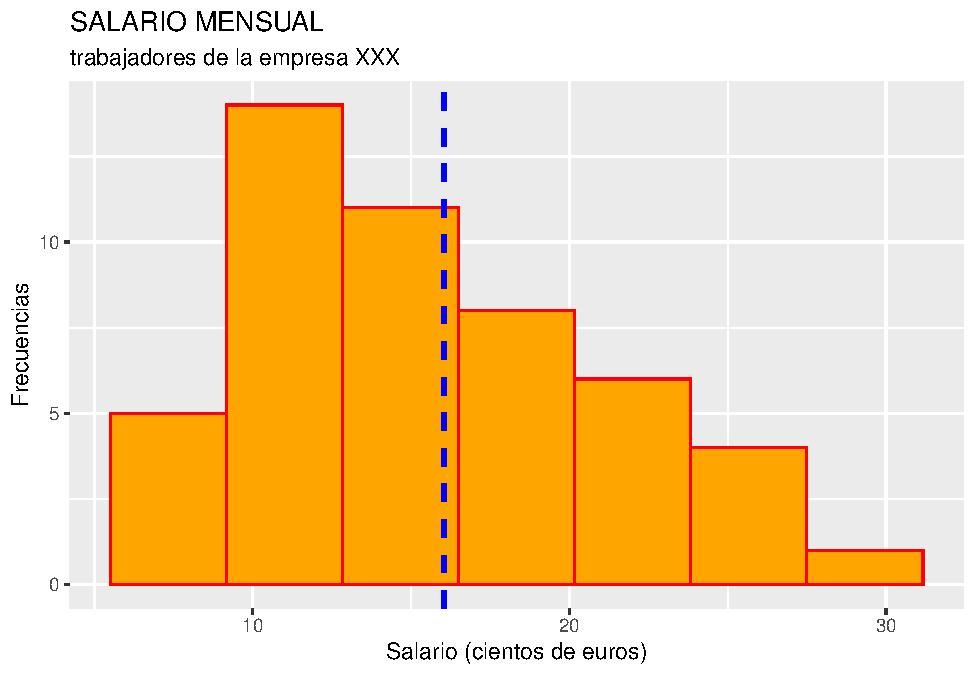
\includegraphics{_main_files/figure-latex/unnamed-chunk-151-1.pdf}

Como comprobamos, la distribución es claramente asimétrica positiva.

En cuanto a las \textbf{medidas de curtosis}, miden el grado de deformación horizontal con respecto a una distribución ``tipo'', la distribución normal.
Suponemos previamente que la distribución de frecuencias estudiada es campaniforme, unimodal y simétrica (o con ligera asimetría).
Pueden darse los casos que se muestran en la figura:

\begin{figure}
\centering
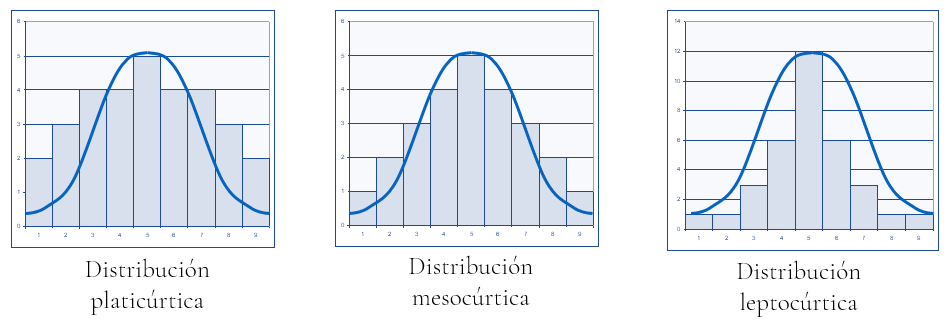
\includegraphics{figuras/curtosis.png}
\caption{Tipos de distribución según el apuntamiento o curtosis}
\end{figure}

El tipo y grado de apuntamiento o curtosis se puede obtener mediante el \textbf{coeficiente de apuntamiento de Fisher}.
Este coeficiente toma valor negativo si la distribución es \emph{platicúrtica} (más aplastada que la distribución normal), valor positivo si la distribución es \emph{leptocúrtica} (más apuntada que la distribución normal), y se acerca a 0 en caso de que la distribución sea aproximadamente igual de apuntada que la distribución normal.
En R, se puede obtener el coeficiente de asimetría mediante la función \texttt{kurtosis()} del paquete \texttt{\{moments\}}.
Hay que tener en cuenta que para que esta versión coincida con lo dicho anteriormente, al valor calculado hay que restarle el valor ``3'':

\begin{Shaded}
\begin{Highlighting}[]
\CommentTok{\# Coeficiente de apuntamiento o curtosis de Fisher}

\NormalTok{curtosis }\OtherTok{\textless{}{-}} \FunctionTok{kurtosis}\NormalTok{(datos}\SpecialCharTok{$}\NormalTok{SALARIO) }\SpecialCharTok{{-}} \DecValTok{3}
\NormalTok{curtosis}
\end{Highlighting}
\end{Shaded}

\begin{verbatim}
## [1] -3.823296
\end{verbatim}

Se aprecia como el coeficiente (corregido) es menor que 0, por lo que la distribución de frecuencias de la variable SALARIO es platicúrtica (más ``aplastada'' que la distribución de frecuencias normal. También hay que tener en cuenta que debemos tener precaución en la aplicación del coeficiente, ya que vimos con anterioridad que la distribución no es aproximadamente simétrica. Gráficamente, podemos comprobar lo anterior representando el histograma y una curva normal que posea la misma moda (que ya calculamos anteriormente).
Para que sean comparables, debemos transformar el eje ``y'' del gráfico, pasando de ``frecuencias'' a ``densidad'', para lo cuál se incluye en el \texttt{geom\_histogram()} el argumento \texttt{aes(y\ =\ ..density..)}:

\begin{Shaded}
\begin{Highlighting}[]
\FunctionTok{ggplot}\NormalTok{(}\AttributeTok{data =}\NormalTok{ datos, }\AttributeTok{map =} \FunctionTok{aes}\NormalTok{(}\AttributeTok{x =}\NormalTok{ SALARIO)) }\SpecialCharTok{+}
  \FunctionTok{geom\_histogram}\NormalTok{(}\AttributeTok{bins =} \DecValTok{7}\NormalTok{, }\AttributeTok{colour =} \StringTok{"red"}\NormalTok{, }\AttributeTok{fill =} \StringTok{"orange"}\NormalTok{, }\FunctionTok{aes}\NormalTok{(}\AttributeTok{y =}\NormalTok{ ..density..)) }\SpecialCharTok{+}
  \FunctionTok{stat\_function}\NormalTok{(}\AttributeTok{fun =}\NormalTok{ dnorm, }\AttributeTok{args =} \FunctionTok{list}\NormalTok{(}\AttributeTok{mean =}\NormalTok{ moda, }\AttributeTok{sd =} \FunctionTok{sd}\NormalTok{(datos}\SpecialCharTok{$}\NormalTok{SALARIO)), }\AttributeTok{colour =} \StringTok{"darkblue"}\NormalTok{, }\AttributeTok{size =} \DecValTok{1}\NormalTok{) }\SpecialCharTok{+}
  \FunctionTok{ggtitle}\NormalTok{(}\StringTok{"SALARIO MENSUAL"}\NormalTok{, }\AttributeTok{subtitle =} \StringTok{"trabajadores de la empresa XXX"}\NormalTok{)}\SpecialCharTok{+}
  \FunctionTok{xlab}\NormalTok{(}\StringTok{"Salario (cientos de euros)"}\NormalTok{) }\SpecialCharTok{+}
  \FunctionTok{ylab}\NormalTok{(}\StringTok{"Densidad"}\NormalTok{)}
\end{Highlighting}
\end{Shaded}

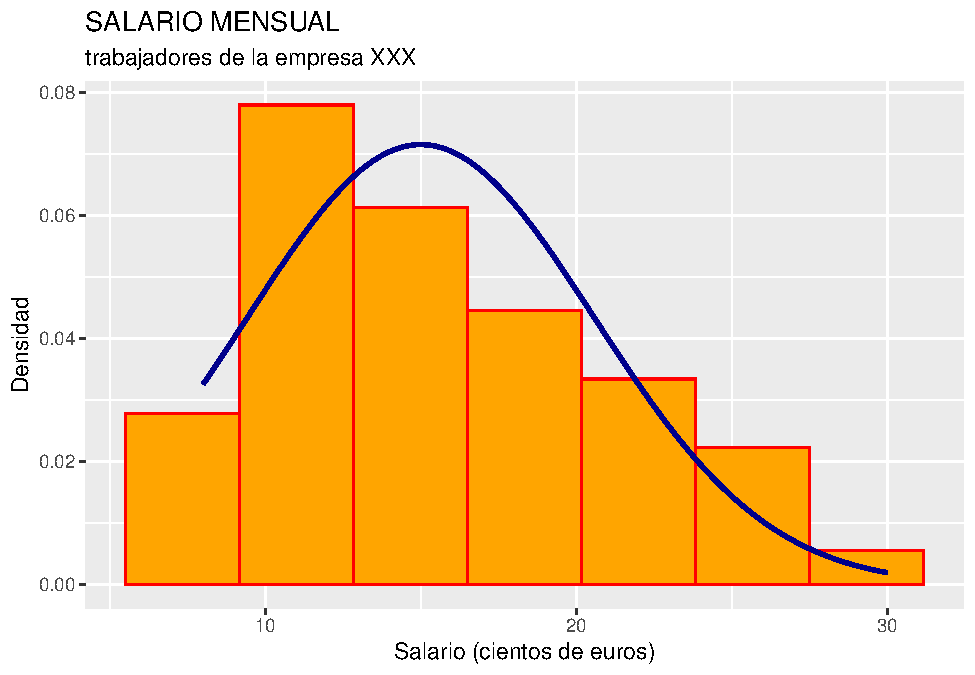
\includegraphics{_main_files/figure-latex/unnamed-chunk-153-1.pdf}

\section{Materiales para realizar las prácticas del capítulo.}\label{materiales-para-realizar-las-pruxe1cticas-del-capuxedtulo.-2}

En esta sección se muestran los links de acceso a los diferentes materiales (\emph{scripts}, datos\ldots) necesarios para llevar a cabo los contenidos prácticos del capítulo.

\textbf{Datos (en formato Microsoft (R) Excel (R)):}

\begin{itemize}
\tightlist
\item
  trabajadores.xlsx (\href{https://docs.google.com/spreadsheets/d/1e_h8P_0sBuD5Nvw6nkeWtXXeiqItFfdI/edit?usp=sharing&ouid=115375878280465826079&rtpof=true&sd=true}{obtener aquí})
\end{itemize}

\textbf{Scripts:}

\begin{itemize}
\tightlist
\item
  explora\_trabajadores.R (\href{https://drive.google.com/file/d/1pfyGPGQRmgOyo9wrZ7fr_KAFj49ecXID/view?usp=sharing}{obtener aquí})
\end{itemize}

\chapter{Análisis previo de datos.}\label{anuxe1lisis-previo-de-datos.}

\section{Introducción.}\label{introducciuxf3n.-1}

Antes de la aplicación de técnicas complejas que permitan extraer de los datos conclusiones relevantes, conviene aplicar a tales datos unos \textbf{pasos iniciales} y técnicas básicas destinadas a conseguir dos objetivos:

\begin{itemize}
\item
  \textbf{Preparar nuestros datos} para que puedan ser procesados correctamente sin provocar distorsiones en los resultados.
\item
  Obtener una \textbf{visión inicial de la información} que esconden nuestros datos, fundamentalmente en cuanto a las medidas básicas que caracterizan la distribución de frecuencias de las variables integradas en nuestros datos, así como, en el caso de contar con más de una variable, de las relaciones que existen entre ellas.
\end{itemize}

Además, es preciso tener en cuenta que, usualmente, es conveniente que estos rasgos iniciales que caracterizan a nuestra muestra o población sean plasmados de un modo \textbf{visualmente amigable}, claro y conciso.

En esta práctica, por medio de un ejemplo basado en información económico-financiera de una muestra constituida por 100 empresas dedicadas a la producción de electricidad mediante tecnología eólica, se mostrarán una serie de buenas prácticas y análisis básicos útiles a la hora de preparar y analizar inicialmente nuestro conjunto de datos.

Vamos a suponer que trabajamos dentro de un \textbf{proyecto} que hemos creado previamente, de nombre ``explora''. Dentro de la carpeta del proyecto guardaremos el \emph{script} llamado ``explora\_describe.R'', y el archivo de Microsoft® Excel® llamado ``eolica\_100\_mv.xlsx''. Si abrimos este último archivo, comprobaremos que se compone de tres hojas. La primera muestra un mensaje sobre el uso de los datos, la segunda recoge la descripción de las variables consideradas, y la tercera (hoja ``Datos'') guarda los datos que debemos importar. Estos datos se corresponden con diferentes variables económico-financieras de las 100 empresas productoras de electricidad mediante generación eólica con mayor volumen de activo.

Luego cerraremos el archivo de Microsoft® Excel®, ``eolica\_100.xlsx'', y volveremos a RStudio. Después, abriremos nuestro \emph{script} ``explora\_describe.R'' con \texttt{File\ →\ Open\ File…} Este \emph{script} contiene el programa que vamos a ir ejecutando en la práctica.

La primera línea / instrucción en el \emph{script} es:

\begin{Shaded}
\begin{Highlighting}[]
\FunctionTok{rm}\NormalTok{(}\AttributeTok{list =} \FunctionTok{ls}\NormalTok{())}
\end{Highlighting}
\end{Shaded}

La instrucción tiene como objeto limpiar el \emph{Environment} (memoria) de objetos de anteriores sesiones de trabajo. Para importar los datos que hay en la hoja ``Datos'' del archivo de Microsoft® Excel® llamado ``eolica\_100\_mv.xlsx'', ejecutaremos el código:

\begin{Shaded}
\begin{Highlighting}[]
\FunctionTok{library}\NormalTok{(readxl)}
\NormalTok{eolica\_100 }\OtherTok{\textless{}{-}} \FunctionTok{read\_excel}\NormalTok{(}\StringTok{"eolica\_100\_mv.xlsx"}\NormalTok{, }\AttributeTok{sheet =} \StringTok{"Datos"}\NormalTok{)}
\FunctionTok{summary}\NormalTok{ (eolica\_100)}
\end{Highlighting}
\end{Shaded}

\begin{verbatim}
##     NOMBRE               RES               ACTIVO             FPIOS        
##  Length:100         Min.   : -5661.5   Min.   :   24944   Min.   : -77533  
##  Class :character   1st Qu.:   669.5   1st Qu.:   34547   1st Qu.:   2305  
##  Mode  :character   Median :  2084.5   Median :   46950   Median :  11936  
##                     Mean   : 11529.8   Mean   :  277270   Mean   : 123743  
##                     3rd Qu.:  3806.7   3rd Qu.:   85610   3rd Qu.:  28292  
##                     Max.   :727548.0   Max.   :13492812   Max.   :6904824  
##                     NA's   :1          NA's   :1                           
## 
##      RENECO           RENFIN            LIQUIDEZ           ENDEUDA       
##  Min.   :-2.813   Min.   :-359.773   Min.   :  0.0140   Min.   :  0.917  
##  1st Qu.: 1.558   1st Qu.:   2.556   1st Qu.:  0.6567   1st Qu.: 50.852  
##  Median : 4.236   Median :  15.326   Median :  1.0650   Median : 83.346  
##  Mean   : 5.416   Mean   :  17.243   Mean   :  2.7214   Mean   : 72.227  
##  3rd Qu.: 7.970   3rd Qu.:  31.307   3rd Qu.:  1.6078   3rd Qu.: 95.388  
##  Max.   :35.262   Max.   : 588.190   Max.   :128.4330   Max.   :140.745  
##  NA's   :2                                              NA's   :2        
## 
##      MARGEN            SOLVENCIA         APALANCA           MATRIZ         
##  Min.   :-2248.157   Min.   :-40.74   Min.   :-8254.11   Length:100        
##  1st Qu.:   12.316   1st Qu.:  4.71   1st Qu.:   16.13   Class :character  
##  Median :   26.618   Median : 16.65   Median :  161.97   Mode  :character  
##  Mean   :    3.228   Mean   : 27.57   Mean   :  345.03                     
##  3rd Qu.:   39.590   3rd Qu.: 45.59   3rd Qu.:  623.13                     
##  Max.   :  400.899   Max.   : 99.08   Max.   :12244.35                     
##  NA's   :2                                                                 
## 
##   DIMENSION        
##  Length:100        
##  Class :character  
##  Mode  :character
\end{verbatim}

R ha considerado la primera columna como una variable de tipo cualitativo, atributo, o factor. En realidad, esta columna no es una variable, sino que está formada por los nombres de los diferentes casos u observaciones. Para evitar que R tome la columna de los nombres de los casos como una variable más, podemos redefinir nuestro \emph{data frame} diciéndole que tome esa primera columna como el conjunto de los \emph{nombres} de los casos:

\begin{Shaded}
\begin{Highlighting}[]
\NormalTok{eolica\_100 }\OtherTok{\textless{}{-}} \FunctionTok{data.frame}\NormalTok{(eolica\_100, }\AttributeTok{row.names =} \DecValTok{1}\NormalTok{)}
\FunctionTok{summary}\NormalTok{ (eolica\_100)}
\end{Highlighting}
\end{Shaded}

\begin{verbatim}
##       RES               ACTIVO             FPIOS             RENECO      
##  Min.   : -5661.5   Min.   :   24944   Min.   : -77533   Min.   :-2.813  
##  1st Qu.:   669.5   1st Qu.:   34547   1st Qu.:   2305   1st Qu.: 1.558  
##  Median :  2084.5   Median :   46950   Median :  11936   Median : 4.236  
##  Mean   : 11529.8   Mean   :  277270   Mean   : 123743   Mean   : 5.416  
##  3rd Qu.:  3806.7   3rd Qu.:   85610   3rd Qu.:  28292   3rd Qu.: 7.970  
##  Max.   :727548.0   Max.   :13492812   Max.   :6904824   Max.   :35.262  
##  NA's   :1          NA's   :1                            NA's   :2       
## 
##      RENFIN            LIQUIDEZ           ENDEUDA            MARGEN         
##  Min.   :-359.773   Min.   :  0.0140   Min.   :  0.917   Min.   :-2248.157  
##  1st Qu.:   2.556   1st Qu.:  0.6567   1st Qu.: 50.852   1st Qu.:   12.316  
##  Median :  15.326   Median :  1.0650   Median : 83.346   Median :   26.618  
##  Mean   :  17.243   Mean   :  2.7214   Mean   : 72.227   Mean   :    3.228  
##  3rd Qu.:  31.307   3rd Qu.:  1.6078   3rd Qu.: 95.388   3rd Qu.:   39.590  
##  Max.   : 588.190   Max.   :128.4330   Max.   :140.745   Max.   :  400.899  
##                                        NA's   :2         NA's   :2          
## 
##    SOLVENCIA         APALANCA           MATRIZ           DIMENSION        
##  Min.   :-40.74   Min.   :-8254.11   Length:100         Length:100        
##  1st Qu.:  4.71   1st Qu.:   16.13   Class :character   Class :character  
##  Median : 16.65   Median :  161.97   Mode  :character   Mode  :character  
##  Mean   : 27.57   Mean   :  345.03                                        
##  3rd Qu.: 45.59   3rd Qu.:  623.13                                        
##  Max.   : 99.08   Max.   :12244.35
\end{verbatim}

Observaremos que ya no aparece NOMBRE, puesto que la columna correspondiente ya no es considerada como una variable.

\section{Análisis de una variable.}\label{anuxe1lisis-de-una-variable.}

\subsection{\texorpdfstring{Buscando \emph{missing values} y \emph{outliers}.}{Buscando missing values y outliers.}}\label{buscando-missing-values-y-outliers.}

Vamos a suponer que la variable que queremos estudiar es la variable \emph{Rentabilidad Económica} (RENECO).

La primera acción que debe realizarse es comprobar que todos los casos (empresas) tienen su correspondiente dato o valor para la variable (RENECO), es decir, que no existen \textbf{valores perdidos o \emph{missing values}}.

Para tener una idea general, se puede utilizar la función \texttt{vis\_miss()} del paquete \texttt{\{visdat\}}, que nos localizará gráficamente los \emph{missing values} de las diferentes variables, y calculará el porcentaje de casos que supone, con respecto al total de observaciones:

\begin{Shaded}
\begin{Highlighting}[]
\FunctionTok{library}\NormalTok{(visdat)}
\FunctionTok{vis\_miss}\NormalTok{(eolica\_100)}
\end{Highlighting}
\end{Shaded}

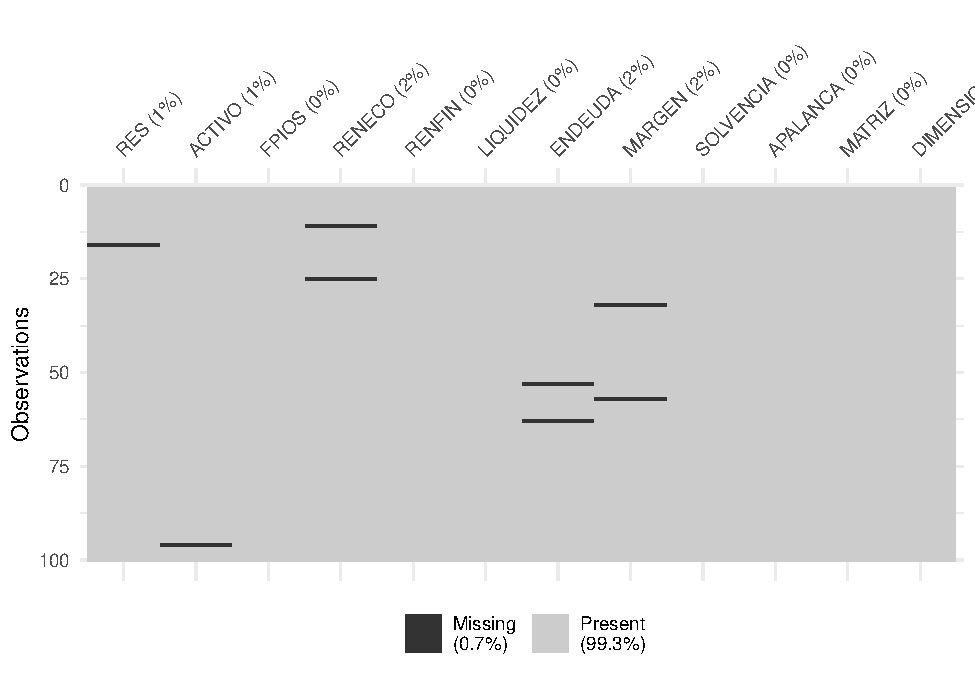
\includegraphics{_main_files/figure-latex/unnamed-chunk-159-1.pdf}

Puede observarse cómo, en el caso concreto de la variable RENECO, un 2\% de los casos no tienen dato (es decir, 2 casos de los 100). Para localizar los casos concretos, puede recurrirse a utilizar las herramientas de manejo de \emph{data frames} del paquete \texttt{\{dplyr\}}. En concreto, realizaremos una copia del \emph{data frame} original, ``eolica\_100'', a la que llamaremos ``muestra'', que es con la que trabajaremos (para mantener la integridad del \emph{data frame} original); y filtraremos los casos para detectar aquellos que carecen de valor en la variable RENECO:

\begin{Shaded}
\begin{Highlighting}[]
\FunctionTok{library}\NormalTok{ (dplyr)}
\NormalTok{muestra}\OtherTok{\textless{}{-}} \FunctionTok{select}\NormalTok{(eolica\_100, }\FunctionTok{everything}\NormalTok{())}
\NormalTok{muestra }\SpecialCharTok{\%\textgreater{}\%} \FunctionTok{filter}\NormalTok{(}\FunctionTok{is.na}\NormalTok{(RENECO)) }\SpecialCharTok{\%\textgreater{}\%} \FunctionTok{select}\NormalTok{(RENECO)}
\end{Highlighting}
\end{Shaded}

La función \texttt{is.na()} comprueba si, en la posición correspondiente a una fila o caso, para la variable escrita en el argumento; hay o no un dato o valor. Como resultado se obtienen dos empresas, para las que se puede comprobar que no hay valor para la variable RENECO:

\begin{verbatim}
##                       RENECO
## Viesgo Renovables SL.     NA
## Sargon Energias SLU       NA
\end{verbatim}

Ante la existencia de \emph{missing values}, se puede actuar de varios modos. Por ejemplo, se puede intentar obtener por otro canal de información el conjunto de valores de RENECO que no están disponibles, o recurrir a alguna estimación para los mismos y asignarlos. En caso de que esto sea difícil, se puede optar, simplemente, por eliminar estos casos, en especial cuando representan un porcentaje muy reducido respecto al total de casos. En nuestro ejemplo, vamos a suponer que hemos optado por esta última vía, al no conseguir unos valores más o menos verosímiles de RENECO para las empresas de las que se carece de dato. Esta \textbf{eliminación de casos} se podrá realizar mediante el código:

\begin{Shaded}
\begin{Highlighting}[]
\NormalTok{muestra }\OtherTok{\textless{}{-}}\NormalTok{ muestra }\SpecialCharTok{\%\textgreater{}\%} \FunctionTok{filter}\NormalTok{(}\SpecialCharTok{!} \FunctionTok{is.na}\NormalTok{(RENECO))}
\end{Highlighting}
\end{Shaded}

El operador \textbf{\texttt{!}} significa ``no''.

Podemos comprobar cómo en el \emph{Global Environment} aparece el \emph{data frame} ``muestra'' con dos casos menos (98):

\begin{figure}
\centering
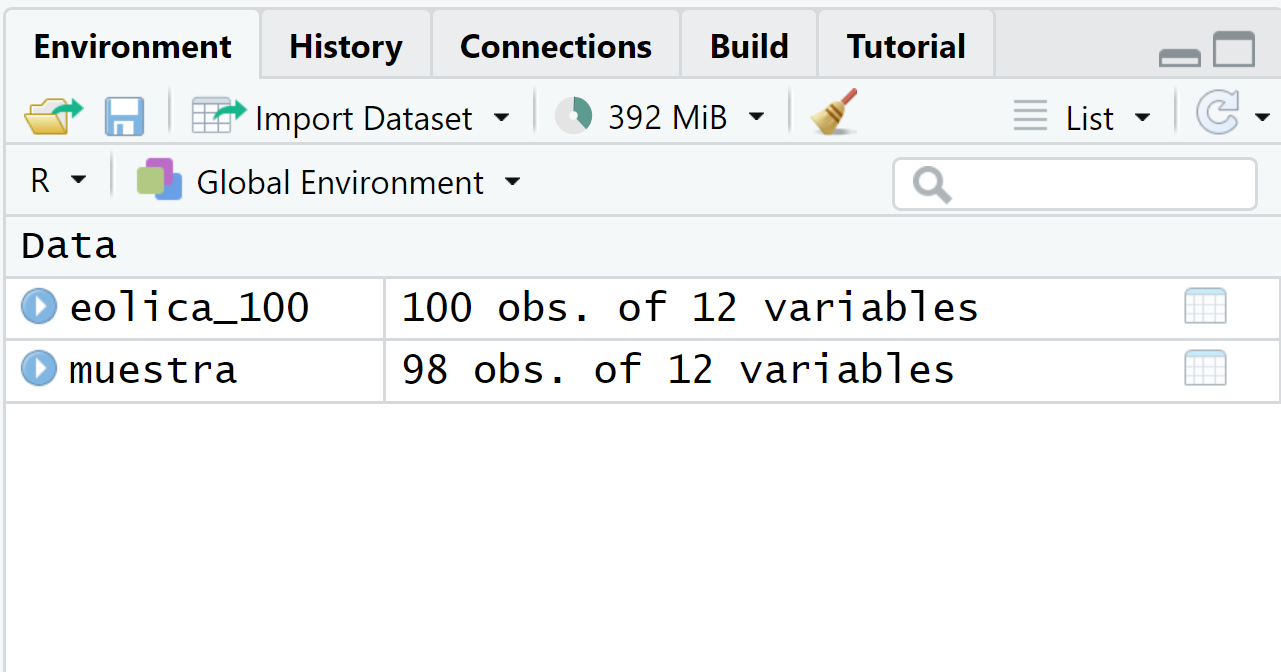
\includegraphics[width=5.20833in,height=\textheight]{figuras/Imagen4_01.png}
\caption{Global Environment.}
\end{figure}

Una vez tratados los casos con valores perdidos o \emph{missing values}, \textbf{conviene detectar la posible presencia de \emph{outliers}} o casos atípicos en la muestra, que pudieran desvirtuar los resultados derivados de ciertos análisis. Al trabajar con una sola variable métrica (la rentabilidad económica, RENECO), podemos intentar realizar esta tarea \textbf{representando gráficamente} la variable mediante un \textbf{\emph{boxplot}} o \emph{gráfico de caja}. Aplicaremos, por ejemplo, el código siguiente, que utiliza la gramática del paquete \texttt{\{ggplot2\}}:

\begin{Shaded}
\begin{Highlighting}[]
\FunctionTok{library}\NormalTok{ (ggplot2)}
\FunctionTok{ggplot}\NormalTok{(}\AttributeTok{data =}\NormalTok{ muestra, }\AttributeTok{map =}\NormalTok{ (}\FunctionTok{aes}\NormalTok{(}\AttributeTok{y =}\NormalTok{ RENECO))) }\SpecialCharTok{+}
    \FunctionTok{geom\_boxplot}\NormalTok{(}\AttributeTok{fill =} \StringTok{"orange"}\NormalTok{) }\SpecialCharTok{+}
    \FunctionTok{ggtitle}\NormalTok{(}\StringTok{"RENTABILIDAD ECONÓMICA"}\NormalTok{, }\AttributeTok{subtitle =} \StringTok{"100 empresas eólicas"}\NormalTok{) }\SpecialCharTok{+}
    \FunctionTok{ylab}\NormalTok{(}\StringTok{"Rentabilidad Económica (\%)"}\NormalTok{)}
\end{Highlighting}
\end{Shaded}

Obteniéndose el gráfico:

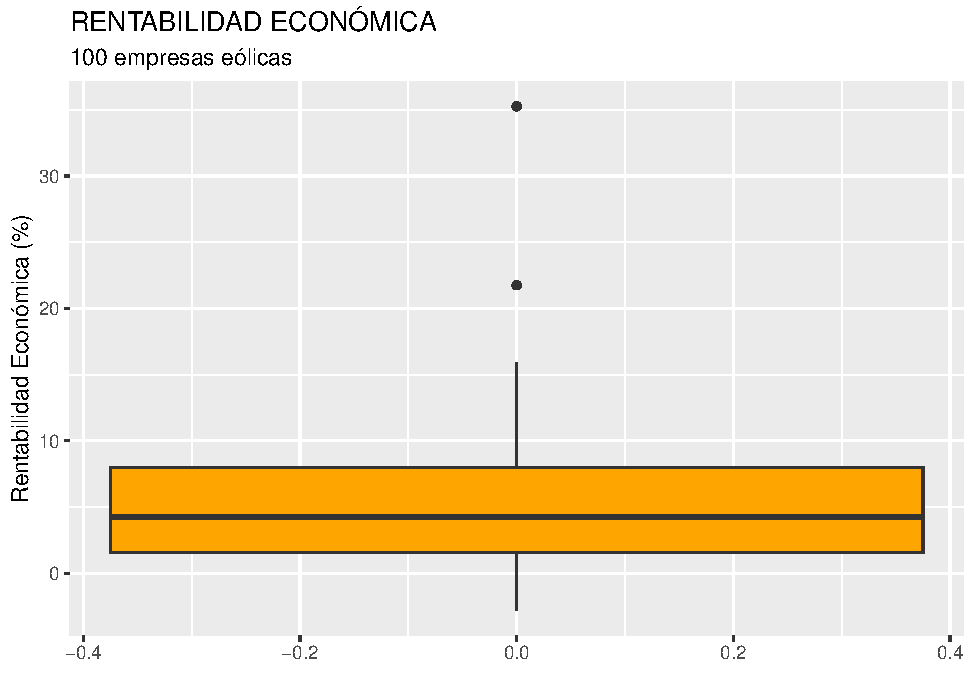
\includegraphics{_main_files/figure-latex/unnamed-chunk-164-1.pdf}

La ``caja'' contiene el 50\% de los casos centrales (los que van del primer cuartil al tercero, cuya diferencia se llama \emph{rango intercuartílico}), y contiene una línea horizontal que es la mediana (segundo cuartil). Por arriba sobresale un segmento que llega al valor de la variable más grande que no llega a ser atípico; y por debajo de la caja otro segmento que llega al valor de la variable más pequeño que no llega a ser atípico. Un valor atípico es el que se aleja más de 1.5 veces el rango intercuartílico (altura de la caja) del tercer cuartil, por arriba; o del primer cuartil, por abajo. Se registran mediante puntos.

En nuestro caso, el \emph{boxplot} ratifica la existencia de dos casos atípicos. Para identificar esos dos casos concretos, podemos recurrir al paquete \texttt{\{dplyr\}}, y \textbf{establecer un filtro} con el siguiente código:

\begin{Shaded}
\begin{Highlighting}[]
\NormalTok{Q1 }\OtherTok{\textless{}{-}} \FunctionTok{quantile}\NormalTok{ (muestra}\SpecialCharTok{$}\NormalTok{RENECO, }\FunctionTok{c}\NormalTok{(}\FloatTok{0.25}\NormalTok{))}
\NormalTok{Q3 }\OtherTok{\textless{}{-}} \FunctionTok{quantile}\NormalTok{ (muestra}\SpecialCharTok{$}\NormalTok{RENECO, }\FunctionTok{c}\NormalTok{(}\FloatTok{0.75}\NormalTok{))}
\NormalTok{muestra }\SpecialCharTok{\%\textgreater{}\%} 
        \FunctionTok{filter}\NormalTok{(RENECO }\SpecialCharTok{\textgreater{}}\NormalTok{ Q3 }\SpecialCharTok{+} \FloatTok{1.5}\SpecialCharTok{*}\FunctionTok{IQR}\NormalTok{(RENECO) }\SpecialCharTok{|}\NormalTok{ RENECO }\SpecialCharTok{\textless{}}\NormalTok{ Q1 }\SpecialCharTok{{-}} \FloatTok{1.5}\SpecialCharTok{*}\FunctionTok{IQR}\NormalTok{(RENECO)) }\SpecialCharTok{\%\textgreater{}\%}
        \FunctionTok{select}\NormalTok{(RENECO)}
\end{Highlighting}
\end{Shaded}

En el código anterior, las dos primeras filas calculan los cuartiles primero (Q1) y tercero (Q3) mediante la función \texttt{quantile()}. Es preciso tener en cuenta que esta función calcula los \emph{percentiles}. Luego se filtran, mediante la función de \texttt{\{dplyr\}} \texttt{filter()}, los \emph{outliers}, calculadoscomo aquellos casos con valores de RENECO mayores que Q3 más 1,5 veces el rango intercuartílico de la variable; o menores que Q1 menos 1,5 veces dicho rango intercuartílico. Para calcular el rango intercuartílico se recurre a la función \texttt{IQR()}. Finalmente, con \texttt{select()}, se muestran los casos en la consola de R-Studio:

\begin{verbatim}
##                     RENECO
## Molinos Del Ebro SA 35.262
## Sierra De Selva SL  21.761
\end{verbatim}

Como ocurría con los \emph{missing values}, el tratamiento de los \emph{outliers} depende de la información que se tenga, existiendo varias alternativas (corrección del dato, estimación, etc.) Si no se tiene información fiable, y los \emph{outliers} no representan una gran proporción respecto al total de casos, puede optarse por su eliminación de la muestra. En este ejemplo, efectivamente, \textbf{eliminaremos estas dos empresas con comportamiento atípico} en la rentabilidad económica (RENECO), a fin de que su presencia en la muestra \textbf{no} \textbf{distorsione los resultados en la aplicación posterior de ciertas técnicas} (por ejemplo, un ANOVA o un análisis de regresión). Podemos hacerlo creando un nuevo \emph{data frame} a partir de ``muestra''; pero sin esos dos casos. Ese nuevo \emph{data frame} se llamará, por ejemplo, ``\textbf{muestra\_so}'':

\begin{Shaded}
\begin{Highlighting}[]
\NormalTok{muestra\_so }\OtherTok{\textless{}{-}}\NormalTok{ muestra }\SpecialCharTok{\%\textgreater{}\%}
            \FunctionTok{filter}\NormalTok{(RENECO }\SpecialCharTok{\textless{}=}\NormalTok{ Q3 }\SpecialCharTok{+} \FloatTok{1.5}\SpecialCharTok{*}\FunctionTok{IQR}\NormalTok{(RENECO) }\SpecialCharTok{\&}\NormalTok{ RENECO }\SpecialCharTok{\textgreater{}=}\NormalTok{ Q1 }\SpecialCharTok{{-}} \FloatTok{1.5}\SpecialCharTok{*}\FunctionTok{IQR}\NormalTok{(RENECO))}
\end{Highlighting}
\end{Shaded}

Es importante observar que, en el código de la función \texttt{filter()}, las desigualdades deben cambiar, así como el operador ``\textbf{\textbar{}}'' por el operador ``\textbf{\&}''. En el \emph{Global Environment} podemos comprobar cómo el \emph{data frame} ``muestra\_so'' posee el mismo número de variables que el \emph{data frame} ``muestra''; pero con dos observaciones o casos menos (96).

\subsection{Descripción de una variable.}\label{descripciuxf3n-de-una-variable.}

Una vez se tiene preparada nuestra base de datos, con un tratamiento adecuado de los \emph{missing values} y de los \emph{outliers,} y \textbf{antes} de proceder a la aplicación de una técnica adecuada, según los objetivos perseguidos en el estudio; suelen presentarse una serie de \textbf{gráficos} básicos y \textbf{medidas} descriptivas que proporcionan una \textbf{idea inicial de la estructura} del sector para la variable o variables analizadas. Nos referimos a medidas y/o gráficos de posición, dispersión y forma (asimetría y curtosis).

El \textbf{análisis gráfico} suele dar una idea atractiva e intuitiva de la estructura de la distribución de frecuencias de nuestro conjunto de casos en relación con la variable a analizar. Un gráfico fundamental es el \textbf{histograma} de la variable estudiada. Para ello, utilizaremos la gramática del paquete \texttt{\{ggplot2\}}:

\begin{Shaded}
\begin{Highlighting}[]
\FunctionTok{ggplot}\NormalTok{(}\AttributeTok{data =}\NormalTok{ muestra\_so, }\AttributeTok{map =} \FunctionTok{aes}\NormalTok{(}\AttributeTok{x =}\NormalTok{ RENECO)) }\SpecialCharTok{+}
  \FunctionTok{geom\_histogram}\NormalTok{(}\AttributeTok{bins =} \DecValTok{40}\NormalTok{,}
                 \AttributeTok{colour =} \StringTok{"red"}\NormalTok{,}
                 \AttributeTok{fill =} \StringTok{"orange"}\NormalTok{,}
                 \AttributeTok{alpha =} \FloatTok{0.7}\NormalTok{) }\SpecialCharTok{+}
  \FunctionTok{geom\_vline}\NormalTok{(}\AttributeTok{xintercept =} \FunctionTok{mean}\NormalTok{(muestra\_so}\SpecialCharTok{$}\NormalTok{RENECO),}
             \AttributeTok{color =} \StringTok{"dark blue"}\NormalTok{,}
             \AttributeTok{size =} \FloatTok{1.2}\NormalTok{,}
             \AttributeTok{alpha =} \FloatTok{0.8}\NormalTok{) }\SpecialCharTok{+}
  \FunctionTok{ggtitle}\NormalTok{(}\StringTok{"RENTABILIDAD ECONÓMICA"}\NormalTok{, }\AttributeTok{subtitle =} \StringTok{"100 empresas eólicas"}\NormalTok{)}\SpecialCharTok{+}
  \FunctionTok{xlab}\NormalTok{(}\StringTok{"Rentabilidad Económica (\%)"}\NormalTok{) }\SpecialCharTok{+}
  \FunctionTok{ylab}\NormalTok{(}\StringTok{"Frecuencias"}\NormalTok{)}
\end{Highlighting}
\end{Shaded}

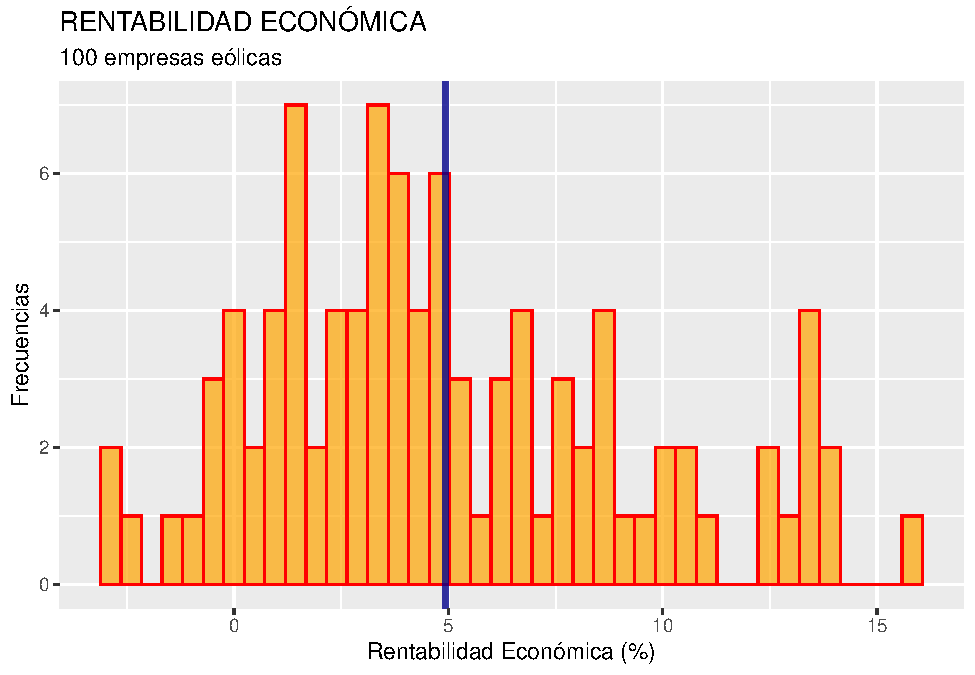
\includegraphics{_main_files/figure-latex/unnamed-chunk-168-1.pdf}

En el gráfico vemos de un modo claro la distribución de frecuencias en cuanto a la rentabilidad económica (RENECO). Se ha incorporado una línea vertical azul (mediante \texttt{geom\_vline()}) para localizar la rentabilidad media. Entre otras cosas, se puede apreciar que la distribución de frecuencias es acampanada y \emph{asimétrica positiva}.

Por otro lado, conviene tener conocimiento del valor de las principales \textbf{medidas descriptivas} (de posición, dispersión, forma) que caracterizan a la distribución de la variable a analizar. Una opción rápida y completa consiste en hacer uso de la función \texttt{descr()} del paquete \texttt{\{summarytools\}}. Así por ejemplo, el código:

\begin{Shaded}
\begin{Highlighting}[]
\FunctionTok{library}\NormalTok{ (summarytools)}
\FunctionTok{descr}\NormalTok{(muestra\_so}\SpecialCharTok{$}\NormalTok{RENECO,}
      \AttributeTok{stats =} \FunctionTok{c}\NormalTok{(}\StringTok{"mean"}\NormalTok{, }\StringTok{"sd"}\NormalTok{, }\StringTok{"min"}\NormalTok{, }\StringTok{"q1"}\NormalTok{, }\StringTok{"med"}\NormalTok{, }\StringTok{"q3"}\NormalTok{, }\StringTok{"max"}\NormalTok{, }\StringTok{"iqr"}\NormalTok{, }\StringTok{"cv"}\NormalTok{),}
      \AttributeTok{transpose =} \ConstantTok{FALSE}\NormalTok{,}
      \AttributeTok{style =} \StringTok{"simple"}\NormalTok{,}
      \AttributeTok{justify =} \StringTok{"center"}\NormalTok{,}
      \AttributeTok{headings =}\NormalTok{ T)}
\end{Highlighting}
\end{Shaded}

Da lugar a la siguiente tabla:

\label{tab:unnamed-chunk-170}Medidas descriptivas

RENECO

Mean

4.9350208

Std.Dev

4.3120451

Min

-2.8130000

Q1

1.4185000

Median

4.1440000

Q3

7.8380000

Max

15.8820000

IQR

6.4002500

CV

0.8737643

Estos valores se corresponden con el valor medio de RENECO, su desviación típica, valor mínimo, primer cuartil, mediana, tercer cuartil, valor máximo, rango intercuartílico, y \emph{coeficiente de variación} o CV, que es una medida de dispersión relativa calculada como la desviación típica entre la media (número de ``medias'' que ``caben'' en una desviación típica. Estas medidas fueron explicadas con detenimiento en el capítulo 4.

\subsection{Normalidad.}\label{normalidad.}

En muchas técnicas multivariantes basadas en métodos inferenciales (por ejemplo, análisis de la varianza, o en la regresión lineal), se requiere que las variables sigan una \textbf{distribución normal}. Para comprobarlo, se puede a recurrir a análisis gráficos o a análisis formales, estos últimos basados en contrastar la hipótesis nula de normalidad.

Vamos a mostrar un \textbf{método gráfico} muy extendido. Comprobaremos la normalidad de la variable RENECO mediante un \textbf{\emph{gráfico qq}} (cuantil-cuantil), que compara los cuantiles de nuestra muestra con los de una distribución normal teórica (con la misma media y desviación típica). Si los puntos se sitúan cercanos a la diagonal, entonces se asumirá un comportamiento (aproximadamente) normal. El código para realizar el gráfico con las herramientas del paquete \texttt{\{ggplot2\}} es:

\begin{Shaded}
\begin{Highlighting}[]
\FunctionTok{ggplot}\NormalTok{(}\AttributeTok{data =}\NormalTok{ muestra\_so, }\FunctionTok{aes}\NormalTok{(}\AttributeTok{sample =}\NormalTok{ RENECO)) }\SpecialCharTok{+}
  \FunctionTok{stat\_qq}\NormalTok{(}\AttributeTok{colour =} \StringTok{"red"}\NormalTok{) }\SpecialCharTok{+} 
  \FunctionTok{stat\_qq\_line}\NormalTok{(}\AttributeTok{colour =} \StringTok{"dark blue"}\NormalTok{) }\SpecialCharTok{+}
  \FunctionTok{ggtitle}\NormalTok{(}\StringTok{"RENTABILIDAD ECONÓMICA: QQ{-}PLOT"}\NormalTok{, }\AttributeTok{subtitle =} \StringTok{"Empresas eólicas"}\NormalTok{)}
\end{Highlighting}
\end{Shaded}

Y el resultado:

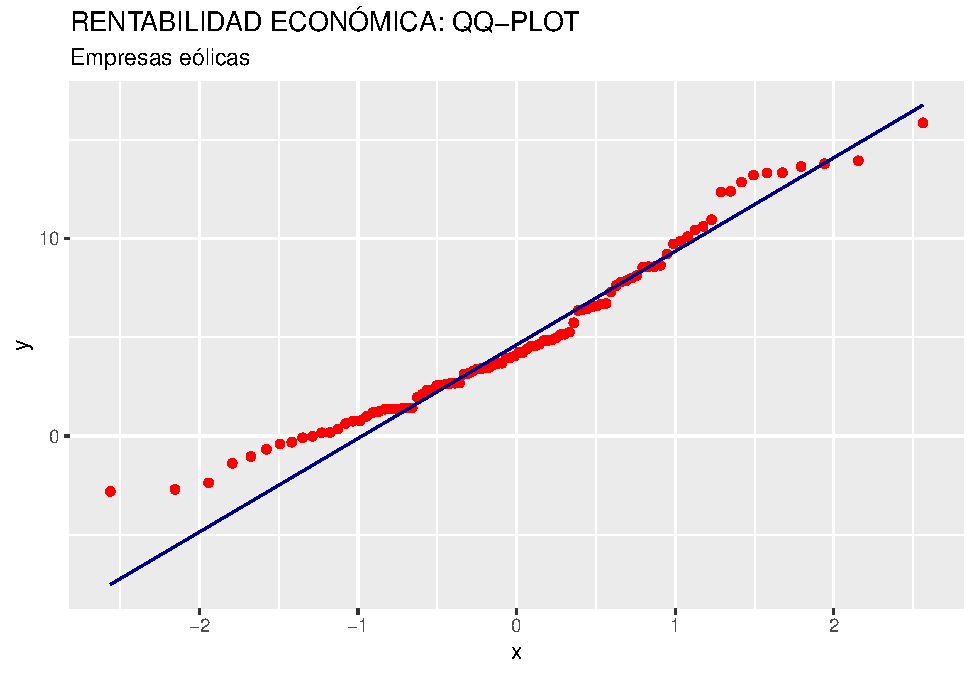
\includegraphics{_main_files/figure-latex/unnamed-chunk-172-1.pdf}

A veces, es difícil obtener una conclusión sólida con el gráfico \emph{qq}; aunque en el ejemplo se aprecia, sobre todo en los primeros puntos, una separación notable de estos con respecto a la línea, lo que induce a pensar en que podría \textbf{no} seguirse una distribución normal.

Si queremos ser más precisos, en lugar de un análisis gráfico se puede recurrir a realizar un análisis formal, basado en la realización de \textbf{contrastes de hipótesis}. Una prueba muy usual es la \textbf{prueba de normalidad de \emph{Shapiro y Wilk}}, que tiene un buen comportamiento en muestras relativamente reducidas. En esta prueba, la hipótesis nula equivale al supuesto de normalidad. Para un 5\% de significación estadística, un p-valor superior a 0.05 implicará el no-rechazo de la hipótesis de normalidad. Para realizar la prueba, se ejecutará el código:

\begin{Shaded}
\begin{Highlighting}[]
\FunctionTok{shapiro.test}\NormalTok{(}\AttributeTok{x =}\NormalTok{ muestra\_so}\SpecialCharTok{$}\NormalTok{RENECO)}
\end{Highlighting}
\end{Shaded}

El resultado obtenido en la consola:

\begin{verbatim}
## 
##  Shapiro-Wilk normality test
## 
## data:  muestra_so$RENECO
## W = 0.9605, p-value = 0.005523
\end{verbatim}

Como el p-valor es (muy) inferior a 0.05, \textbf{se rechaza la hipótesis nula de normalidad en la distribución}, lo que implica que, para una significación estadística del 5\%, admitimos que RENECO \textbf{no} sigue, para nuestra muestra, un comportamiento normal, como ya se anticipó con el gráfico \emph{qq}.

\section{Análisis de múltiples variables.}\label{anuxe1lisis-de-muxfaltiples-variables.}

Son muchas las técnicas aplicadas al análisis de datos económicos basadas en una distribución de frecuencias multivariante. En este apartado nos centraremos en el caso de \textbf{variables métricas}, ya que al caso de atributos, variables categóricas o factores; le dedicaremos un tema en exclusiva. Algunas técnicas multivariantes son el análisis de componentes principales, el análisis de regresión, el análisis clúster\ldots{}

Todas estas metodologías requieren, de nuevo, de una fase inicial que ponga a punto la base de datos y ofrezca una fotografía de cómo es la situación en cuanto a las variables en estudio. En este sentido, es conveniente aplicar, para cada variable por separado, algunos de los análisis gráficos básicos vistos anteriormente.

A estos análisis básicos hay que añadir, principalmente, algún estudio gráfico y alguna medida cuantitativa más, destinados fundamentalmente a comprobar el \textbf{grado de intensidad en la relación estadística} entre las variables implicadas. Antes de abordar esta última cuestión, trabajaremos con dos variables.

\subsection{Caso de dos variables: localización de missing values y outliers, y representación gráfica.}\label{caso-de-dos-variables-localizaciuxf3n-de-missing-values-y-outliers-y-representaciuxf3n-gruxe1fica.}

En nuestro ejemplo, vamos a incorporar al análisis la variable ACTIVO (\emph{volumen de activos de la empresa en miles de euros}). Partiremos, como ya hicimos en el caso univariante, de la detección de valores perdidos o \emph{missing values}. Para no modificar el \emph{data frame} original (``eolica\_100''), trabajaremos con una copia, llamada ``muestra2'':

\begin{Shaded}
\begin{Highlighting}[]
\NormalTok{muestra2 }\OtherTok{\textless{}{-}} \FunctionTok{select}\NormalTok{(eolica\_100, }\FunctionTok{everything}\NormalTok{())}
\NormalTok{muestra2 }\SpecialCharTok{\%\textgreater{}\%} \FunctionTok{filter}\NormalTok{(}\FunctionTok{is.na}\NormalTok{(RENECO) }\SpecialCharTok{|} \FunctionTok{is.na}\NormalTok{(ACTIVO)) }\SpecialCharTok{\%\textgreater{}\%}
  \FunctionTok{select}\NormalTok{(RENECO, ACTIVO)}
\end{Highlighting}
\end{Shaded}

El operador \textbf{\texttt{\textbar{}}} significa ``o''.

Con el código anterior se obtiene en la consola:

\begin{verbatim}
##                              RENECO ACTIVO
## Viesgo Renovables SL.            NA 269730
## Sargon Energias SLU              NA  85745
## La Caldera Energia Burgos SL  2.643     NA
\end{verbatim}

Como ya se discutió anteriormente, si comprobamos que los \emph{missing values} no pueden ser obtenidos o estimados mediante alguna otra vía, y son relativamente pocas observaciones, se podría optar por eliminarlos. Vamos a suponer en este ejemplo, que ese es el caso:

\begin{Shaded}
\begin{Highlighting}[]
\NormalTok{muestra2 }\OtherTok{\textless{}{-}}\NormalTok{ muestra2 }\SpecialCharTok{\%\textgreater{}\%} \FunctionTok{filter}\NormalTok{(}\SpecialCharTok{!} \FunctionTok{is.na}\NormalTok{(RENECO) }\SpecialCharTok{\&} \SpecialCharTok{!} \FunctionTok{is.na}\NormalTok{(ACTIVO) )}
\end{Highlighting}
\end{Shaded}

El operador \textbf{\texttt{\&}} significa ``y''.

El \emph{data frame} ``muestra2'' contiene los mismos datos que ``eolica\_100'', salvo los tres casos con \emph{missing values} (97).

Se pasaría ahora a detectar los posibles \emph{outliers}. Al trabajar con dos variables, una posibilidad cómoda para extraer una conclusión inicial es generar un \textbf{gráfico de dispersión}. Utilizando la gramática de ggplot2:

\begin{Shaded}
\begin{Highlighting}[]
\CommentTok{\# Localizando outliers}

\NormalTok{dispersion }\OtherTok{\textless{}{-}} \FunctionTok{ggplot}\NormalTok{(}\AttributeTok{data =}\NormalTok{ muestra2, }\AttributeTok{map =}\NormalTok{ (}\FunctionTok{aes}\NormalTok{(}\AttributeTok{x =}\NormalTok{ RENECO,}
                                                 \AttributeTok{y =}\NormalTok{ ACTIVO}\SpecialCharTok{/}\DecValTok{100000}\NormalTok{))) }\SpecialCharTok{+} 
              \FunctionTok{geom\_point}\NormalTok{(}\AttributeTok{colour =} \StringTok{"red"}\NormalTok{, }\AttributeTok{size =} \DecValTok{2}\NormalTok{, }\AttributeTok{alpha =} \FloatTok{0.5}\NormalTok{) }\SpecialCharTok{+}
              \FunctionTok{ggtitle}\NormalTok{(}\StringTok{"RENTABILIDAD ECONÓMICA vs ACTIVO"}\NormalTok{,}
                      \AttributeTok{subtitle =} \StringTok{"100 empresas eólicas"}\NormalTok{) }\SpecialCharTok{+} 
              \FunctionTok{xlab}\NormalTok{(}\StringTok{"Rentabilidad Económica (\%)"}\NormalTok{) }\SpecialCharTok{+} 
              \FunctionTok{ylab}\NormalTok{(}\StringTok{"Activo (cientos de millones de euros)"}\NormalTok{) }
\NormalTok{dispersion}
\end{Highlighting}
\end{Shaded}

Puede apreciarse cómo en el ``mapeo'' de las coordenadas, el ACTIVO aparece divido entre 100.000. Esto es simplemente para aminorar la escala del eje ``y'', y dotar de una escala más cómoda (visible) al gráfico. Eso ha hecho que en la etiqueta de este gráfico pongamos ``cientos de milllones de euros'', en lugar de ``miles de euros'', que son las unidades de la variable ACTIVO. Por otro lado, el gráfico se ha asignado, primeramente, al objeto ``dispersion'', al que se ha llamado con posterioridad.

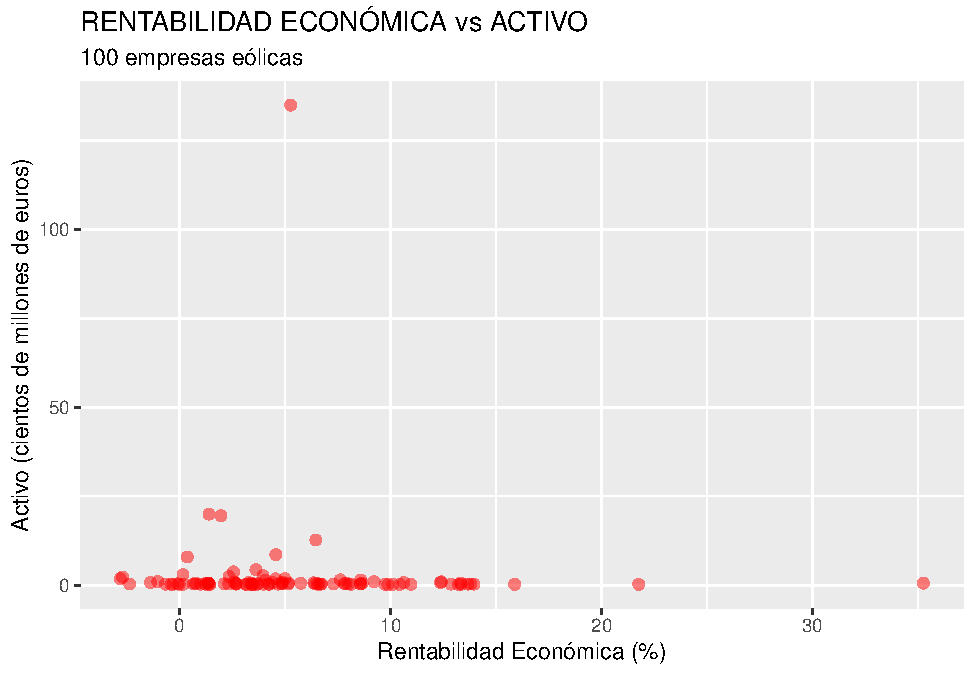
\includegraphics{_main_files/figure-latex/unnamed-chunk-179-1.pdf}

En el gráfico se distinguen varios puntos muy alejados del resto, que son candidatos a ser \emph{outliers}.

Además, podríamos crear los gráficos de caja para cada una de las variables. Estos gráficos los vamos a asignar a dos objetos, ``caja\_RENECO'' y ``caja\_ACTIVO''. Posteriormente, con las facilidades del paquete \texttt{\{patchwork\}} se combinarán los tres gráficos, a fin de proporcionar una presentación más compacta. El código es el siguiente:

\begin{Shaded}
\begin{Highlighting}[]
\NormalTok{caja\_RENECO }\OtherTok{\textless{}{-}} \FunctionTok{ggplot}\NormalTok{(}\AttributeTok{data =}\NormalTok{ muestra2, }\AttributeTok{map =}\NormalTok{ (}\FunctionTok{aes}\NormalTok{(}\AttributeTok{y =}\NormalTok{ RENECO))) }\SpecialCharTok{+}
               \FunctionTok{geom\_boxplot}\NormalTok{(}\AttributeTok{fill =} \StringTok{"orange"}\NormalTok{) }\SpecialCharTok{+}
               \FunctionTok{ggtitle}\NormalTok{(}\StringTok{"RENTABILIDAD ECONÓMICA"}\NormalTok{,}
                       \AttributeTok{subtitle =} \StringTok{"100 empresas eólicas"}\NormalTok{) }\SpecialCharTok{+}
               \FunctionTok{ylab}\NormalTok{(}\StringTok{"Rentabilidad Económica (\%)"}\NormalTok{)}

\NormalTok{caja\_ACTIVO }\OtherTok{\textless{}{-}} \FunctionTok{ggplot}\NormalTok{(}\AttributeTok{data =}\NormalTok{ muestra2, }\AttributeTok{map =}\NormalTok{ (}\FunctionTok{aes}\NormalTok{(}\AttributeTok{y =}\NormalTok{ ACTIVO}\SpecialCharTok{/}\DecValTok{100000}\NormalTok{))) }\SpecialCharTok{+}
               \FunctionTok{geom\_boxplot}\NormalTok{(}\AttributeTok{fill =} \StringTok{"orange"}\NormalTok{) }\SpecialCharTok{+}
               \FunctionTok{ggtitle}\NormalTok{(}\StringTok{"ACTIVO"}\NormalTok{,}
                       \AttributeTok{subtitle =} \StringTok{"100 empresas eólicas"}\NormalTok{) }\SpecialCharTok{+}
               \FunctionTok{ylab}\NormalTok{(}\StringTok{"Activo (cientos de millones de euros)"}\NormalTok{)}
\FunctionTok{library}\NormalTok{ (patchwork)}
\NormalTok{dispersion }\SpecialCharTok{/}\NormalTok{ (caja\_RENECO }\SpecialCharTok{|}\NormalTok{ caja\_ACTIVO)}
\end{Highlighting}
\end{Shaded}

Y el resultado:

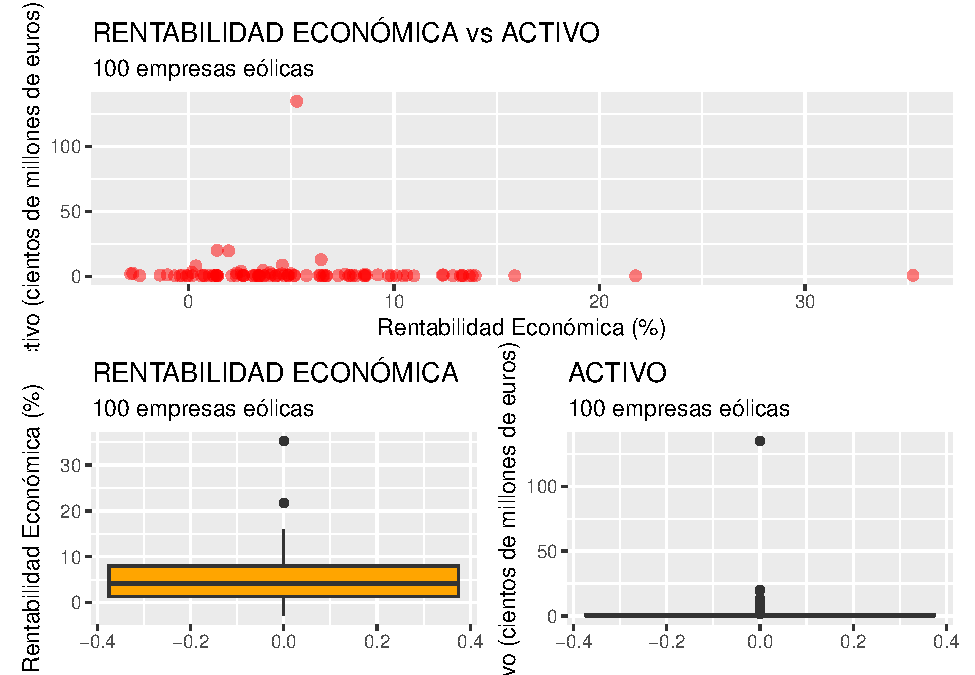
\includegraphics{_main_files/figure-latex/unnamed-chunk-181-1.pdf}

La última línea de código, mediante el paquete \texttt{\{patchwork\}}, maqueta la visualización de los tres gráficos. El operador \texttt{/} indica que los gráficos siguientes se dispondrán inmediatamente debajo; mientras que \texttt{\textbar{}} indica que el gráfico siguiente se dispone al lado del anterior.

Lo más destacable es, en el caso de la variable ACTIVO, cómo el diagrama de caja confirma la existencia de \emph{outliers}, con un caso muy claro.

Vamos a suponer que se decide eliminar los \emph{outliers} de la muestra, a fin de evitar distorsiones en los resultados de la posterior aplicación de alguna técnica. El código para localizar los \emph{outliers} será:

\begin{Shaded}
\begin{Highlighting}[]
\NormalTok{Q1\_RENECO }\OtherTok{\textless{}{-}} \FunctionTok{quantile}\NormalTok{ (muestra2}\SpecialCharTok{$}\NormalTok{RENECO, }\FunctionTok{c}\NormalTok{(}\FloatTok{0.25}\NormalTok{))}
\NormalTok{Q3\_RENECO }\OtherTok{\textless{}{-}} \FunctionTok{quantile}\NormalTok{ (muestra2}\SpecialCharTok{$}\NormalTok{RENECO, }\FunctionTok{c}\NormalTok{(}\FloatTok{0.75}\NormalTok{))}
\NormalTok{Q1\_ACTIVO }\OtherTok{\textless{}{-}} \FunctionTok{quantile}\NormalTok{ (muestra2}\SpecialCharTok{$}\NormalTok{ACTIVO, }\FunctionTok{c}\NormalTok{(}\FloatTok{0.25}\NormalTok{))}
\NormalTok{Q3\_ACTIVO }\OtherTok{\textless{}{-}} \FunctionTok{quantile}\NormalTok{ (muestra2}\SpecialCharTok{$}\NormalTok{ACTIVO, }\FunctionTok{c}\NormalTok{(}\FloatTok{0.75}\NormalTok{))}

\NormalTok{muestra2 }\SpecialCharTok{\%\textgreater{}\%}
  \FunctionTok{filter}\NormalTok{(RENECO }\SpecialCharTok{\textgreater{}}\NormalTok{ Q3\_RENECO }\SpecialCharTok{+} \FloatTok{1.5}\SpecialCharTok{*}\FunctionTok{IQR}\NormalTok{(RENECO) }\SpecialCharTok{|}
\NormalTok{           RENECO }\SpecialCharTok{\textless{}}\NormalTok{ Q1\_RENECO }\SpecialCharTok{{-}} \FloatTok{1.5}\SpecialCharTok{*}\FunctionTok{IQR}\NormalTok{(RENECO) }\SpecialCharTok{|}
\NormalTok{           ACTIVO }\SpecialCharTok{\textgreater{}}\NormalTok{ Q3\_ACTIVO }\SpecialCharTok{+} \FloatTok{1.5}\SpecialCharTok{*}\FunctionTok{IQR}\NormalTok{(ACTIVO) }\SpecialCharTok{|}
\NormalTok{           ACTIVO }\SpecialCharTok{\textless{}}\NormalTok{ Q1\_ACTIVO }\SpecialCharTok{{-}} \FloatTok{1.5}\SpecialCharTok{*}\FunctionTok{IQR}\NormalTok{(ACTIVO)) }\SpecialCharTok{\%\textgreater{}\%}
  \FunctionTok{select}\NormalTok{(RENECO, ACTIVO)}
\end{Highlighting}
\end{Shaded}

Con lo que, en la consola, se listarán los siguientes casos:

\begin{verbatim}
##                                RENECO      ACTIVO
## Holding De Negocios De GAS SL.  5.264 13492812.00
## Global Power Generation SA.     1.393  2002458.00
## Naturgy Renovables SLU          1.959  1956869.00
## EDP Renovables España SLU       6.458  1275939.00
## Corporacion Acciona Eolica SL   4.562   864606.00
## Saeta Yield SA.                 0.360   796886.38
## Elawan Energy SL.               3.615   443467.00
## Olivento SL                     2.553   381206.98
## Parque Eolico La Boga SL.       0.162   303904.36
## Naturgy Wind, S.L.              3.949   273542.00
## Al-Andalus Wind Power SL        2.349   249853.83
## Innogy Spain SA.               -2.708   230338.51
## Guzman Energia SL              -2.813   190286.98
## Acciona Eolica Del Levante SL   4.985   188354.00
## Biovent Energia SA              4.551   183899.00
## Esquilvent SL                   7.621   157630.62
## Molinos Del Ebro SA            35.262    62114.37
## Sierra De Selva SL             21.761    27728.00
\end{verbatim}

Son 18 casos. Vamos a eliminarlos de la muestra, pero creando un nuevo \emph{data frame}, ``muestra2\_so'', para conservar el anterior:

\begin{Shaded}
\begin{Highlighting}[]
\NormalTok{muestra2\_so }\OtherTok{\textless{}{-}}\NormalTok{ muestra2 }\SpecialCharTok{\%\textgreater{}\%}
  \FunctionTok{filter}\NormalTok{(RENECO }\SpecialCharTok{\textless{}=}\NormalTok{ Q3\_RENECO }\SpecialCharTok{+} \FloatTok{1.5}\SpecialCharTok{*}\FunctionTok{IQR}\NormalTok{(RENECO) }\SpecialCharTok{\&}
\NormalTok{           RENECO }\SpecialCharTok{\textgreater{}=}\NormalTok{ Q1\_RENECO }\SpecialCharTok{{-}} \FloatTok{1.5}\SpecialCharTok{*}\FunctionTok{IQR}\NormalTok{(RENECO) }\SpecialCharTok{\&}
\NormalTok{           ACTIVO }\SpecialCharTok{\textless{}=}\NormalTok{ Q3\_ACTIVO }\SpecialCharTok{+} \FloatTok{1.5}\SpecialCharTok{*}\FunctionTok{IQR}\NormalTok{(ACTIVO) }\SpecialCharTok{\&}
\NormalTok{           ACTIVO }\SpecialCharTok{\textgreater{}=}\NormalTok{ Q1\_ACTIVO }\SpecialCharTok{{-}} \FloatTok{1.5}\SpecialCharTok{*}\FunctionTok{IQR}\NormalTok{(ACTIVO))}
\end{Highlighting}
\end{Shaded}

Si se construyen ahora los gráficos anteriores; pero con ``muestra2\_so'', que ya no incluye \emph{outliers}, se comprobará el cambio que experimentan tales gráficos:

\begin{Shaded}
\begin{Highlighting}[]
\NormalTok{dispersion\_so }\OtherTok{\textless{}{-}} \FunctionTok{ggplot}\NormalTok{(}\AttributeTok{data =}\NormalTok{ muestra2\_so, }\AttributeTok{map =}\NormalTok{ (}\FunctionTok{aes}\NormalTok{(}\AttributeTok{x =}\NormalTok{ RENECO,}
                                                       \AttributeTok{y =}\NormalTok{ ACTIVO}\SpecialCharTok{/}\DecValTok{100000}\NormalTok{))) }\SpecialCharTok{+} 
  \FunctionTok{geom\_point}\NormalTok{(}\AttributeTok{colour =} \StringTok{"red"}\NormalTok{, }\AttributeTok{size =} \DecValTok{2}\NormalTok{, }\AttributeTok{alpha =} \FloatTok{0.5}\NormalTok{) }\SpecialCharTok{+}
  \FunctionTok{ggtitle}\NormalTok{(}\StringTok{"RENTABILIDAD ECONÓMICA vs ACTIVO"}\NormalTok{,}
          \AttributeTok{subtitle =} \StringTok{"100 empresas eólicas"}\NormalTok{) }\SpecialCharTok{+} 
  \FunctionTok{xlab}\NormalTok{(}\StringTok{"Rentabilidad Económica (\%)"}\NormalTok{) }\SpecialCharTok{+} 
  \FunctionTok{ylab}\NormalTok{(}\StringTok{"Activo (cientos de millones de euros)"}\NormalTok{) }

\NormalTok{caja\_RENECO\_so }\OtherTok{\textless{}{-}} \FunctionTok{ggplot}\NormalTok{(}\AttributeTok{data =}\NormalTok{ muestra2\_so, }\AttributeTok{map =}\NormalTok{ (}\FunctionTok{aes}\NormalTok{(}\AttributeTok{y =}\NormalTok{ RENECO))) }\SpecialCharTok{+}
  \FunctionTok{geom\_boxplot}\NormalTok{(}\AttributeTok{fill =} \StringTok{"orange"}\NormalTok{) }\SpecialCharTok{+}
  \FunctionTok{ggtitle}\NormalTok{(}\StringTok{"RENTABILIDAD ECONÓMICA"}\NormalTok{,}
          \AttributeTok{subtitle =} \StringTok{"100 empresas eólicas"}\NormalTok{) }\SpecialCharTok{+}
  \FunctionTok{ylab}\NormalTok{(}\StringTok{"Rentabilidad Económica (\%)"}\NormalTok{)}

\NormalTok{caja\_ACTIVO\_so }\OtherTok{\textless{}{-}} \FunctionTok{ggplot}\NormalTok{(}\AttributeTok{data =}\NormalTok{ muestra2\_so, }\AttributeTok{map =}\NormalTok{ (}\FunctionTok{aes}\NormalTok{(}\AttributeTok{y =}\NormalTok{ ACTIVO}\SpecialCharTok{/}\DecValTok{100000}\NormalTok{))) }\SpecialCharTok{+}
  \FunctionTok{geom\_boxplot}\NormalTok{(}\AttributeTok{fill =} \StringTok{"orange"}\NormalTok{) }\SpecialCharTok{+}
  \FunctionTok{ggtitle}\NormalTok{(}\StringTok{"ACTIVO"}\NormalTok{,}
          \AttributeTok{subtitle =} \StringTok{"100 empresas eólicas"}\NormalTok{) }\SpecialCharTok{+}
  \FunctionTok{ylab}\NormalTok{(}\StringTok{"Activo (cientos de millones de euros)"}\NormalTok{)}

\NormalTok{dispersion\_so }\SpecialCharTok{/}\NormalTok{ (caja\_RENECO\_so }\SpecialCharTok{|}\NormalTok{ caja\_ACTIVO\_so)}
\end{Highlighting}
\end{Shaded}

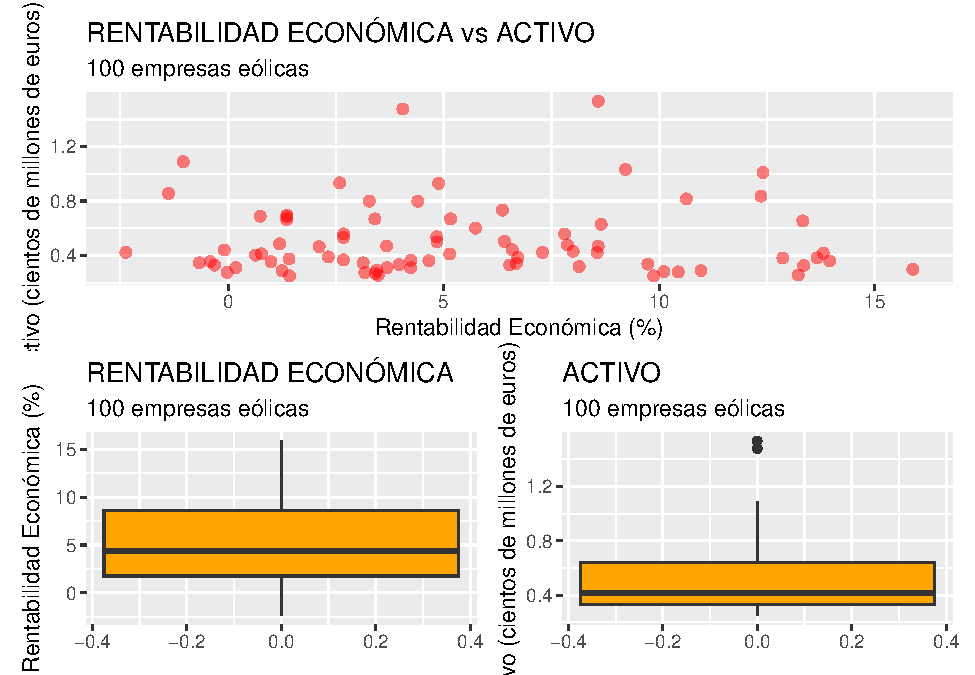
\includegraphics{_main_files/figure-latex/unnamed-chunk-185-1.pdf}

Aunque vuelven a aparecer dos \emph{outliers} en la variable ACTIVO, en el gráfico de dispersión se aprecia una nube de puntos más homogénea que antes de haber eliminado los casos u observaciones localizados con anterioridad.

\subsection{Caso de múltiples variables.}\label{caso-de-muxfaltiples-variables.}

Si las variables que entran en nuestro análisis son más de dos (suponemos que todas están en escala métrica), la detección y, en su caso, eliminación de \emph{missing values} será un proceso semejante al de los casos anteriores.

Por ejemplo, vamos a imaginar que queremos realizar un análisis en el que tendremos en cuenta las variables RENECO (rentabilidad económica), ACTIVO (volumen de activos de la empresa), MARGEN (margen de beneficio) y RES (resultado del ejercicio).

Para detectar los \emph{missing values} procederemos creando una copia del \emph{data frame} original (para preservarlo), llamada ``muestra3'' y ejecutando el código:

\begin{Shaded}
\begin{Highlighting}[]
\NormalTok{muestra3 }\OtherTok{\textless{}{-}} \FunctionTok{select}\NormalTok{(eolica\_100, }\FunctionTok{everything}\NormalTok{())}
\NormalTok{muestra3 }\SpecialCharTok{\%\textgreater{}\%} \FunctionTok{filter}\NormalTok{(}\FunctionTok{is.na}\NormalTok{(RENECO) }\SpecialCharTok{|}
                      \FunctionTok{is.na}\NormalTok{(ACTIVO) }\SpecialCharTok{|}
                      \FunctionTok{is.na}\NormalTok{(MARGEN) }\SpecialCharTok{|}
                      \FunctionTok{is.na}\NormalTok{(RES)) }\SpecialCharTok{\%\textgreater{}\%}
  \FunctionTok{select}\NormalTok{(RENECO, ACTIVO, MARGEN, RES)}
\end{Highlighting}
\end{Shaded}

El listado de casos con \emph{missing values} será:

\begin{verbatim}
##                              RENECO    ACTIVO   MARGEN       RES
## Viesgo Renovables SL.            NA 269730.00   11.818  4609.000
## Biovent Energia SA            4.551 183899.00   22.792        NA
## Sargon Energias SLU              NA  85745.00 -615.625 -2216.000
## Parc Eolic Sant Antoni SL     1.361  69654.00       NA   668.000
## Eolica La Brujula SA          7.295  42146.98       NA  2306.062
## La Caldera Energia Burgos SL  2.643        NA   14.448   511.304
\end{verbatim}

Para eliminar estos casos (siempre que no se hayan podido obtener por otra vía o estimar) utilizaremos el código:

El \emph{data frame} ``muestra3'' contiene los mismos datos que ``eolica\_100'', salvo los 6 casos con \emph{missing values} (94).

Para la detección de posibles \emph{outliers}, al haber más de 2 variables, ya no puede utilizarse un gráfico de dispersión, porque implicaría más de dos ejes. Además, si las variables que entran en el análisis son numerosas, podría ser poco operativo estudiar las variables una a una. Una alternativa consiste en calcular la \textbf{\emph{distancia de Mahalanobis}} de las variables del estudio, como \textbf{``resumen'' del comportamiento de cada caso} en todas las variables del análisis. Así, primero vamos a calcular un vector con los valores de la \emph{distancia de} \emph{Mahalanobis} del conjunto de las 4 variables en cada uno de los casos (empresas eólicas). Este vector lo denominaremos, por ejemplo, MAHALANOBIS\emph{.} Una vez calculado, lo añadiremos al \emph{data frame} ``muestra3'' mediante la función de pegado de columnas, \texttt{cbind()}:

\begin{Shaded}
\begin{Highlighting}[]
\CommentTok{\#Detectando y eliminando outliers.}

\NormalTok{muestra3.variables }\OtherTok{\textless{}{-}}\NormalTok{ muestra3 }\SpecialCharTok{\%\textgreater{}\%} \FunctionTok{select}\NormalTok{(RENECO, ACTIVO, MARGEN, RES)}
\NormalTok{MAHALANOBIS }\OtherTok{\textless{}{-}}\FunctionTok{mahalanobis}\NormalTok{(muestra3.variables,}
                          \AttributeTok{center =} \FunctionTok{colMeans}\NormalTok{(muestra3.variables),}
                          \AttributeTok{cov =} \FunctionTok{cov}\NormalTok{(muestra3.variables))}
\NormalTok{muestra3 }\OtherTok{\textless{}{-}} \FunctionTok{cbind}\NormalTok{(muestra3, MAHALANOBIS)}
\end{Highlighting}
\end{Shaded}

Posteriormente, se puede construir el diagrama de caja de la variable MAHALANOBIS, como cualquier otra variable:

\begin{Shaded}
\begin{Highlighting}[]
\FunctionTok{ggplot}\NormalTok{(}\AttributeTok{data =}\NormalTok{ muestra3, }\AttributeTok{map =}\NormalTok{ (}\FunctionTok{aes}\NormalTok{(}\AttributeTok{y =}\NormalTok{ MAHALANOBIS))) }\SpecialCharTok{+}
    \FunctionTok{geom\_boxplot}\NormalTok{(}\AttributeTok{fill =} \StringTok{"orange"}\NormalTok{) }\SpecialCharTok{+}
    \FunctionTok{ggtitle}\NormalTok{(}\StringTok{"DISTANCIA DE MAHALANOBIS"}\NormalTok{,}
            \AttributeTok{subtitle =} \StringTok{"RENECO, ACTIVO, MARGEN, RES. 100 empresas eólicas "}\NormalTok{) }\SpecialCharTok{+}
    \FunctionTok{ylab}\NormalTok{(}\StringTok{"MAHALANOBIS"}\NormalTok{)}
\end{Highlighting}
\end{Shaded}

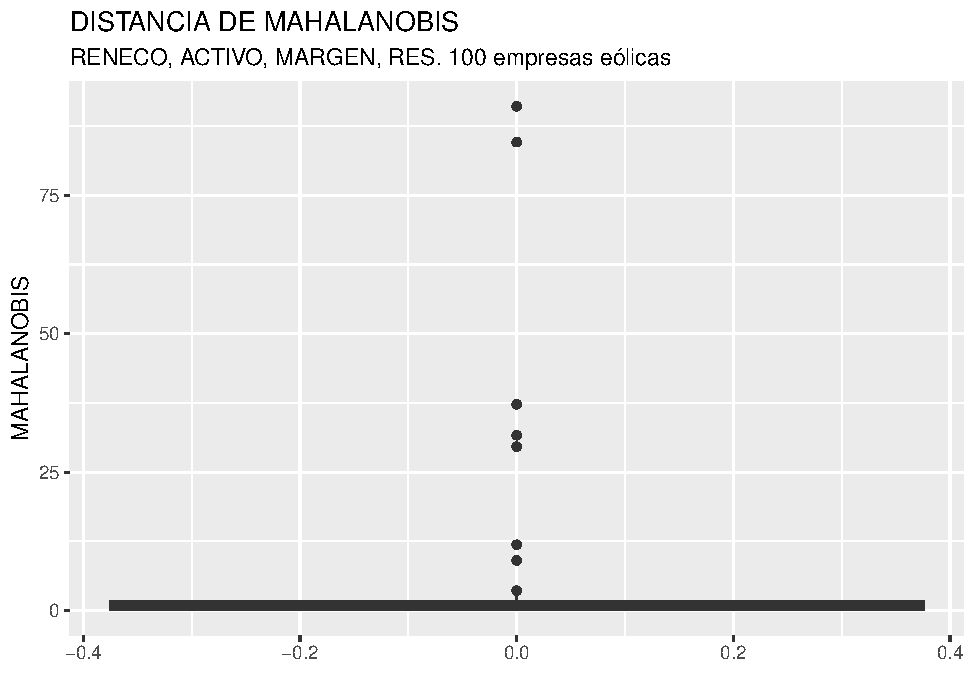
\includegraphics{_main_files/figure-latex/unnamed-chunk-190-1.pdf}

Para saber de qué casos concretos se trata, se podrá ejecutar el código:

\begin{Shaded}
\begin{Highlighting}[]
\NormalTok{Q1M }\OtherTok{\textless{}{-}} \FunctionTok{quantile}\NormalTok{ (muestra3}\SpecialCharTok{$}\NormalTok{MAHALANOBIS, }\FunctionTok{c}\NormalTok{(}\FloatTok{0.25}\NormalTok{))}
\NormalTok{Q3M }\OtherTok{\textless{}{-}} \FunctionTok{quantile}\NormalTok{ (muestra3}\SpecialCharTok{$}\NormalTok{MAHALANOBIS, }\FunctionTok{c}\NormalTok{(}\FloatTok{0.75}\NormalTok{))}

\NormalTok{muestra3 }\SpecialCharTok{\%\textgreater{}\%}
  \FunctionTok{filter}\NormalTok{(MAHALANOBIS }\SpecialCharTok{\textgreater{}}\NormalTok{ Q3M }\SpecialCharTok{+} \FloatTok{1.5}\SpecialCharTok{*}\FunctionTok{IQR}\NormalTok{(MAHALANOBIS) }\SpecialCharTok{|}
\NormalTok{           MAHALANOBIS }\SpecialCharTok{\textless{}}\NormalTok{ Q1M }\SpecialCharTok{{-}} \FloatTok{1.5}\SpecialCharTok{*}\FunctionTok{IQR}\NormalTok{(MAHALANOBIS)) }\SpecialCharTok{\%\textgreater{}\%}
  \FunctionTok{select}\NormalTok{(MAHALANOBIS, RENECO, ACTIVO, MARGEN, RES)}
\end{Highlighting}
\end{Shaded}

En la consola se obtendrá el listado:

\begin{verbatim}
##                                MAHALANOBIS RENECO      ACTIVO
## Holding De Negocios De GAS SL.   91.041690  5.264 13492812.00
## Global Power Generation SA.      37.255573  1.393  2002458.00
## Naturgy Renovables SLU           31.675561  1.959  1956869.00
## Saeta Yield SA.                  11.891027  0.360   796886.38
## Molinos Del Ebro SA              29.589696 35.262    62114.37
## Tarraco Eolica SA                 3.600426 12.868    38102.00
## WPD Parque Eolico Navillas SL.   84.589929 -0.416    35511.45
## Brulles Eolica SL                 3.599069 15.882    29722.58
## Sierra De Selva SL                9.055155 21.761    27728.00
## 
##                                   MARGEN         RES
## Holding De Negocios De GAS SL.    91.152 727548.0000
## Global Power Generation SA.       22.403  39995.0000
## Naturgy Renovables SLU            20.442  42737.0000
## Saeta Yield SA.                   16.258   2084.4760
## Molinos Del Ebro SA               41.821  17026.2569
## Tarraco Eolica SA                400.899   4953.0000
## WPD Parque Eolico Navillas SL. -2248.157   -110.9293
## Brulles Eolica SL                 47.227   3540.5693
## Sierra De Selva SL                47.045   4525.0000
\end{verbatim}

Si se opta por eliminar estos casos cara al análisis posterior, se podrá crear un nuevo \emph{data frame}, por ejemplo ``muestra3\_so'', con el código siguiente:

\begin{Shaded}
\begin{Highlighting}[]
\NormalTok{muestra3\_so }\OtherTok{\textless{}{-}}\NormalTok{ muestra3 }\SpecialCharTok{\%\textgreater{}\%}
  \FunctionTok{filter}\NormalTok{(MAHALANOBIS }\SpecialCharTok{\textless{}=}\NormalTok{ Q3M }\SpecialCharTok{+} \FloatTok{1.5}\SpecialCharTok{*}\FunctionTok{IQR}\NormalTok{(MAHALANOBIS) }\SpecialCharTok{\&}
\NormalTok{           MAHALANOBIS }\SpecialCharTok{\textgreater{}=}\NormalTok{ Q1M }\SpecialCharTok{{-}} \FloatTok{1.5}\SpecialCharTok{*}\FunctionTok{IQR}\NormalTok{(MAHALANOBIS))}
\end{Highlighting}
\end{Shaded}

El \emph{data frame} ``muestra3\_so'' será una réplica de ``muestra3'', aunque sin incluir los casos detectados como atípicos o \emph{outliers} (85 casos).

\subsection{Correlación entre variables.}\label{correlaciuxf3n-entre-variables.}

Cuando trabajamos con más de una variable, una característica muy importante viene dada por la intensidad con la que tales variables están relacionadas estadísticamente entre sí, es decir, el estudio de las correlaciones. Un modo atractivo y rápido de visualizar la \textbf{matriz de correlaciones} de las variables es a través de la función \texttt{chart.Correlation()} del paquete \texttt{\{PerformanceAnalytics\}}. Previamente, hemos creado el \emph{data frame} ``muestra3\_so\_variables'' con sola las variables (métricas) del estudio:

\begin{Shaded}
\begin{Highlighting}[]
\CommentTok{\# Correlaciones.}

\NormalTok{muestra3\_so\_variables }\OtherTok{\textless{}{-}}\NormalTok{ muestra3\_so }\SpecialCharTok{\%\textgreater{}\%}
  \FunctionTok{select}\NormalTok{(RENECO, ACTIVO, MARGEN, RES)}

\FunctionTok{library}\NormalTok{(PerformanceAnalytics)}
\FunctionTok{chart.Correlation}\NormalTok{(muestra3\_so\_variables, }\AttributeTok{histogram =}\NormalTok{ F, }\AttributeTok{pch =} \DecValTok{18}\NormalTok{)}
\end{Highlighting}
\end{Shaded}

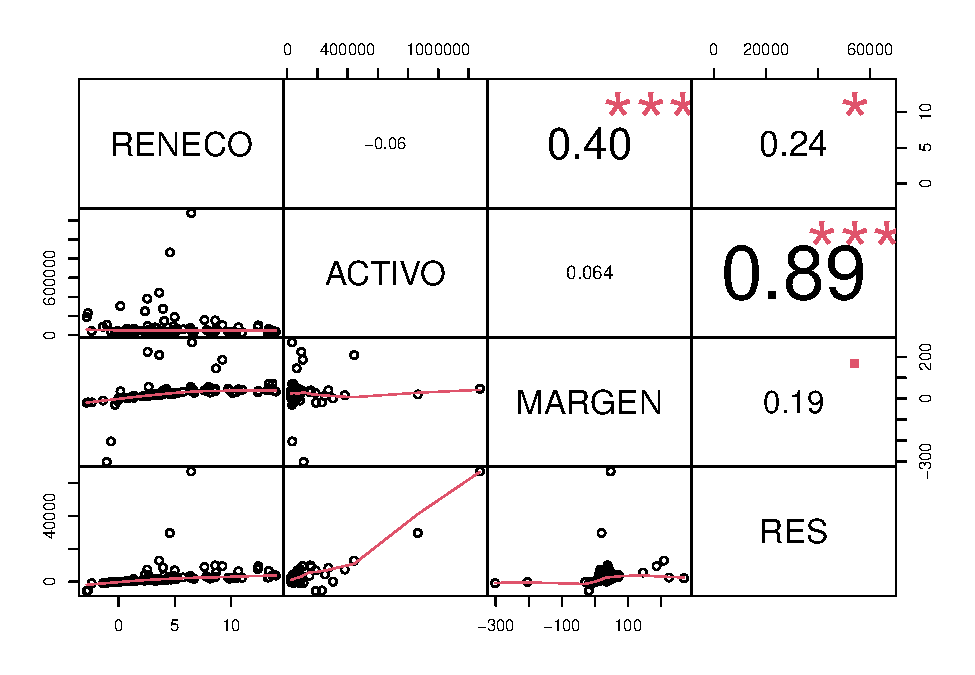
\includegraphics{_main_files/figure-latex/unnamed-chunk-194-1.pdf}

Un coeficiente de correlación puede tomar un valor entre -1 (fuerte relación, en sentido opuesto) a 1 (fuerte relación, en el mismo sentido). Como puede apreciarse en el gráfico, las variables ACTIVO y RES mantienen una relación muy intensa y en sentido positivo. Entre MARGEN y RENECO existe también una relación de intensidad destacable. En cambio, ACTIVO y MARGEN; y RENECO y ACTIVO apenas están estadísticamente relacionadas.

\section{Materiales para realizar las prácticas del capítulo.}\label{materiales-para-realizar-las-pruxe1cticas-del-capuxedtulo.-3}

En esta sección se muestran los links de acceso a los diferentes materiales (scripts, datos\ldots) necesarios para llevar a cabo los contenidos prácticos del capítulo.

\textbf{Datos (en formato Microsoft (R) Excel (R)):}

\begin{itemize}
\tightlist
\item
  eolica\_100\_mv.xlsx (\href{https://docs.google.com/spreadsheets/d/1kgJaXiowfrHy77bKaLxUBuQWfmCcoydU/edit?usp=drive_link&ouid=115375878280465826079&rtpof=true&sd=true}{obtener aquí})
\end{itemize}

\textbf{Scripts:}

\begin{itemize}
\tightlist
\item
  explora\_describe.R (\href{https://drive.google.com/file/d/1eBcJnXpEi-9V6DxbXN7tSToJpGLH2xlB/view?usp=drive_link}{obtener aquí})
\end{itemize}

\chapter{Análisis de la varianza.}\label{anuxe1lisis-de-la-varianza.}

\chapter{Componentes Principales.}\label{componentes-principales.}

\chapter{Análisis Clúster.}\label{anuxe1lisis-cluxfaster.}

\section{Introducción.}\label{introducciuxf3n.-2}

El análisis de conglomerados o análisis clúster (AC) trata de clasificar individuos o casos asignándolos a grupos homogéneos, de manera que:

\begin{itemize}
\item
  Cada grupo, conglomerado o clúster contenga a \textbf{los casos más parecidos} entre sí, en términos de una serie de variables (\textbf{variables clasificadoras}).
\item
  \textbf{Los grupos} contengan casos que, en general, \textbf{sean muy diferentes} a los casos del resto de grupos, de acuerdo con las variables consideradas.
\end{itemize}

En general, el proceso de determinación de los grupos, conglomerados o clústeres de casos es el siguiente:

\begin{itemize}
\tightlist
\item
  Se parte de un conjunto de \textbf{n} casos, y para cada uno de ellos se cuenta con el valor de \textbf{m} variables clasificadoras.
\item
  Se establece una \textbf{medida de distancia} que cuantifica lo que dos casos se parecen, \textbf{considerando en conjunto} los valores que poseen para las variables clasificadoras.
\item
  Se crean los grupos, conglomerados o clústeres con los casos que poseen entre sí una \textbf{menor distancia}. Existen dos \textbf{enfoques} principales a la hora de crear los grupos de casos a partir de las distancias observadas entre los casos: los \emph{métodos jerárquicos} y los \emph{métodos no-jerárquicos}.
\item
  Finalmente, se \textbf{caracterizan} los grupos, conglomerados o clíusteres obtenidos, y se comparan unos con otros para extraer conclusiones.
\end{itemize}

En lo que respecta a la medida de \textbf{distancia} entre los casos, la medida más habitual es la \textbf{distancia euclídea}. Así, la distancia euclídea entre dos caso, i e i', para las m variables clasificadoras x, será:

\[
d(i, i') = \sqrt{\sum_{j=1}^{m} (x_{ij} - x_{i'j})^2}
\] Esta distancia es muy sensible a la escala de las variables clasificadoras. Para evitar este inconveniente, se trabaja con las variables previamente \textbf{tipificadas}.

\section{Métodos de agrupación jerárquicos.}\label{muxe9todos-de-agrupaciuxf3n-jeruxe1rquicos.}

Como se acaba de comentar, existen dos enfoques fundamentales de realizar el análisis clúster, dependiendo de cómo son los métodos de agrupación de los casos (y grupos de casos): el enfoque de los métodos jerárquicos, y el enfoque que reúne a los métodos no-jerárquicos.

Ambos enfoques tienen sus ventajas e inconvenientes, y pueden adaptarse mejor a cada problema concreto. Es importante seleccionar un buen método de agrupación, puesto que pueden proporcionar soluciones muy diferentes entre sí.

En los \textbf{métodos jerárquicos,} se van formando sucesivamente grupos como agrupación de otros grupos precedentes, hasta llegar a un único grupo que recoge a todos los individuos; tomando el proceso una \textbf{estructura piramidal} (también existen métodos jerárquicos descendientes, que parten de un único grupo que contiene a todos los casos, para acabar el n grupos de un solo caso, aunque son menos frecuentes).

Estos métodos suelen aplicarse cuando hay un número reducido de casos. También, cuando nuestro objetivo pasa por crear \textbf{grupos que recojan a todos los casos}, más que definir simplemente tipologías más o menos homogéneas de casos (lo que se obtiene caracterizando los grupos obtenidos). Es decir, cuando se incluyen en el análisis a todos los individuos, incluidos los \emph{outliers}. De hecho, estos métodos pueden emplearse, de por sí, como técnicas de localización de \emph{outliers}. Por último, también se suelen emplearse cuando se desconoce a priori el número de grupos, conglomerados o clústeres a formar.

Entre los métodos jerárquicos de agrupación más extendidos, figuran los siguientes:

\begin{itemize}
\item
  \textbf{Método del vecino más cercano (single linkage):} la distancia que se considera entre grupos es la distancia entre sus elementos más próximos.
\item
  \textbf{Método del vecino más lejano (complete linkage):} la distancia que se considera entre grupos es la distancia entre sus elementos más lejanos.
\item
  \textbf{Método de Ward (Ward method):} se unen los grupos que dan lugar a otro grupo cuyos casos tienen una menor suma de los cuadrados de sus distancias respecto al centro de dicho grupo (menor varianza).
\item
  \textbf{Otros métodos:} vinculación intergrupos (average linkage between groups), vinculación intragrupos (whithin group)\ldots{}
\end{itemize}

De entre ellos, ¿cuál elegir?

La cuestión no es fácil de resolver, y no tiene por qué tener una única respuesta. Por otro lado, cada método proporciona soluciones que pueden variar mucho entre sí. Una estrategia puede pasar por probar con varios métodos y se seleccionar la solución que parezca más coherente desde el punto de vista teórico, y estable desde el punto de vista empírico.

En la práctica, uno de los métodos más utilizados es el \textbf{método de Ward}, porque proporciona grupos muy homogéneos, ya que se basa en la minimización de la varianza o dispersión de los elementos que componen cada grupo con respecto a su centro de gravedad o \textbf{centroide.} Precisamente, este método será aplicado en el ejemplo práctico que desarrollaremos en R a continuación.

\chapter{Tablas de Contingencia.}\label{tablas-de-contingencia.}

\chapter{Análisis de Correspondencias.}\label{anuxe1lisis-de-correspondencias.}

\chapter*{Bibliografía}\label{bibliografuxeda}
\addcontentsline{toc}{chapter}{Bibliografía}

\phantomsection\label{refs}
\begin{CSLReferences}{1}{0}
\bibitem[\citeproctext]{ref-Hernandez2000}
Hernández-Alonso, J. 2000. \emph{Economía Cuantitativa}. Síntesis.

\bibitem[\citeproctext]{ref-Intriligatoretal1996}
Intriligator, R. G.; Hsiao, M. D.; Bodkin. 1996. \emph{Econometric Models, Techniques and Applications}. Prentice-Hall.

\bibitem[\citeproctext]{ref-MartinPliego2004}
Martín-Pliego, F. J. 2004. \emph{Introducción a La Estadística Económica y Empresarial}. Thomson/Paraninfo.

\bibitem[\citeproctext]{ref-Moodux26Graybill1963}
Mood, F. A., A. M.; Graybill. 1963. \emph{Introduction to the Theory of Statistics (2nd Edition)}. Mc Graw-Hill.

\bibitem[\citeproctext]{ref-Peuxf1a1983}
Peña, D. 1983. {``La Influencia de Las Teorías de Newton y Darwin En El Nacimiento de La Estadística Matemática.''} \emph{Estadística Española} 99: 103--4.

\bibitem[\citeproctext]{ref-R-base}
R Core Team. 2024. \emph{R: A Language and Environment for Statistical Computing}. Vienna, Austria: R Foundation for Statistical Computing. \url{https://www.R-project.org/}.

\bibitem[\citeproctext]{ref-Samuelsonux26Nordhaus2006}
Samuelson, W. D., P. A.; Nordhaus. 2006. \emph{Microeconomía (18ª Edición)}. Mc Graw Hill.

\bibitem[\citeproctext]{ref-ggplot22021}
Wickham, Hadley. 2021. \emph{Ggplot2: Elegant Graphics for Data Analysis, 3 Ed.} Springer-Verlag New York. \url{https://ggplot2-book.org/}.

\bibitem[\citeproctext]{ref-Wickham2017R}
Wickham, Hadley, and Garrett Grolemund. 2017. \emph{R for Data Science: Import, Tidy, Transform, Visualize, and Model Data}. 1st ed. Paperback; O'Reilly Media. \url{http://r4ds.had.co.nz/}.

\end{CSLReferences}

\end{document}
